\documentclass[aspectratio=169,11pt]{beamer}

% Theme configuration
\usetheme{Madrid}
\usecolortheme{default}
\setbeamertemplate{navigation symbols}{}
\setbeamertemplate{footline}[frame number]

% Required packages
\usepackage{graphicx}
\usepackage{booktabs}
\usepackage{amsmath}
\usepackage{amssymb}
\usepackage{hyperref}
\usepackage{tikz}
\usepackage{algorithm}
\usepackage{algpseudocode}
\usepackage[normalem]{ulem}

% Title information
\title{Natural Language Processing}
\subtitle{Course Overview and Introduction}
\author{Florian Valade}
\date{\today}

\begin{document}

% Title slide
\begin{frame}
    \titlepage
\end{frame}

\begin{frame}
    \frametitle{Présentation}
    \textbf{Florian Valade} \newline
    \href{mailto:florian.valade@univ-eiffel.fr}{florian.valade@univ-eiffel.fr} \newline
    Data Scientist chez Fujitsu \newline
    Chercheur au LAMA \newline
    \begin{columns}
        \begin{column}{0.5\textwidth}
            \begin{flushleft}
                
\includegraphics[width=0.3\textwidth]{images/lama.png}
            \end{flushleft}
        \end{column}
        \begin{column}{0.5\textwidth}
            \begin{flushright}
                
\includegraphics[width=0.3\textwidth]{images/fujitsu.png}
            \end{flushright}
        \end{column}
    \end{columns}
\end{frame}

% À qui s'adresse ce cours
\begin{frame}{À qui s'adresse ce cours}
    \begin{itemize}
        \item \textbf{Étudiants souhaitant devenir Data Scientists ou ML Engineers}
        \begin{itemize}
            \item Se spécialiser dans les problématiques de langage
            \item Acquérir des compétences recherchées en entreprise
            \item Développer une expertise en analyse de données textuelles
        \end{itemize}
        \vspace{0.3cm}
        \item \textbf{Étudiants intéressés par la recherche en NLP}
        \begin{itemize}
            \item Comprendre les fondements théoriques
            \item Explorer les architectures avancées
            \item Préparer un parcours en recherche
        \end{itemize}
        \vspace{0.3cm}
        \item \textbf{Étudiants curieux de comprendre le fonctionnement des LLMs}
        \begin{itemize}
            \item Démystifier les modèles comme GPT, BERT, LLaMA...
            \item Comprendre les capacités et limites actuelles
        \end{itemize}
    \end{itemize}
\end{frame}

% Objectifs du cours
\begin{frame}{Objectifs du cours}
    \begin{itemize}
        \item \textbf{Comprendre ce qu'est le langage naturel et comment l'analyser}
        \begin{itemize}
            \item Structure linguistique et particularités du langage humain
            \item Défis spécifiques au traitement automatique
            \item Évaluation des systèmes de NLP
        \end{itemize}
        \vspace{0.3cm}
        \item \textbf{Maîtriser les méthodes classiques de NLP}
        \begin{itemize}
            \item Prétraitement et représentation du texte
            \item Vectorisation et modèles statistiques
            \item Classification, extraction d'information et clustering
        \end{itemize}
        \vspace{0.3cm}
        \item \textbf{Explorer les modèles de langage avancés (LLMs)}
        \begin{itemize}
            \item Architectures basées sur l'attention (Transformers)
            \item Préentraînement et fine-tuning
            \item Applications et cas d'usage pratiques
        \end{itemize}
    \end{itemize}
\end{frame}

% Table of contents
\begin{frame}{Plan du cours}
    \tableofcontents
\end{frame}

% Introduction section
\section{Introduction au Traitement du Langage Naturel}

% First slide: Definition of NLP
\begin{frame}{Qu'est-ce que le NLP?}

    \begin{itemize}
        \item Le \textbf{Traitement du Langage Naturel (NLP)} est un domaine de l'intelligence artificielle qui se concentre sur l'interaction entre les ordinateurs et le langage humain
        \item Il vise à permettre aux machines de \textbf{comprendre}, \textbf{interpréter} et \textbf{générer} du langage humain
        \item Le langage est \textbf{omniprésent} dans notre monde:
        \begin{itemize}
            \item Livres, articles et documents
            \item Contenus web et réseaux sociaux
            \item Messages et conversations
            \item Emails et communications professionnelles
        \end{itemize}
        \item Le NLP nous permet d'exploiter et de donner du sens à cette ressource abondante
    \end{itemize}

\end{frame}

% Second slide: Applications of NLP - Text Understanding
\begin{frame}{Applications du NLP: Compréhension de texte}
    \begin{columns}
        \begin{column}{0.55\textwidth}
            \begin{itemize}
                \item \textbf{Analyse de sentiment}
                \begin{itemize}
                    \item Détection des opinions positives/négatives
                    \item Modération automatique des commentaires
                    \item Analyse des retours clients et avis
                \end{itemize}
                \vspace{0.3cm}
                \item \textbf{Classification de texte}
                \begin{itemize}
                    \item Catégorisation des emails (spam/non-spam)
                    \item Organisation des documents par thème
                    \item Filtrage de contenu inapproprié
                \end{itemize}
                \vspace{0.3cm}
                \item \textbf{Extraction d'information}
                \begin{itemize}
                    \item Reconnaissance d'entités nommées (noms, lieux, dates)
                    \item Extraction de relations entre entités
                    \item Résumé automatique de documents
                \end{itemize}
            \end{itemize}
        \end{column}
        \begin{column}{0.45\textwidth}
            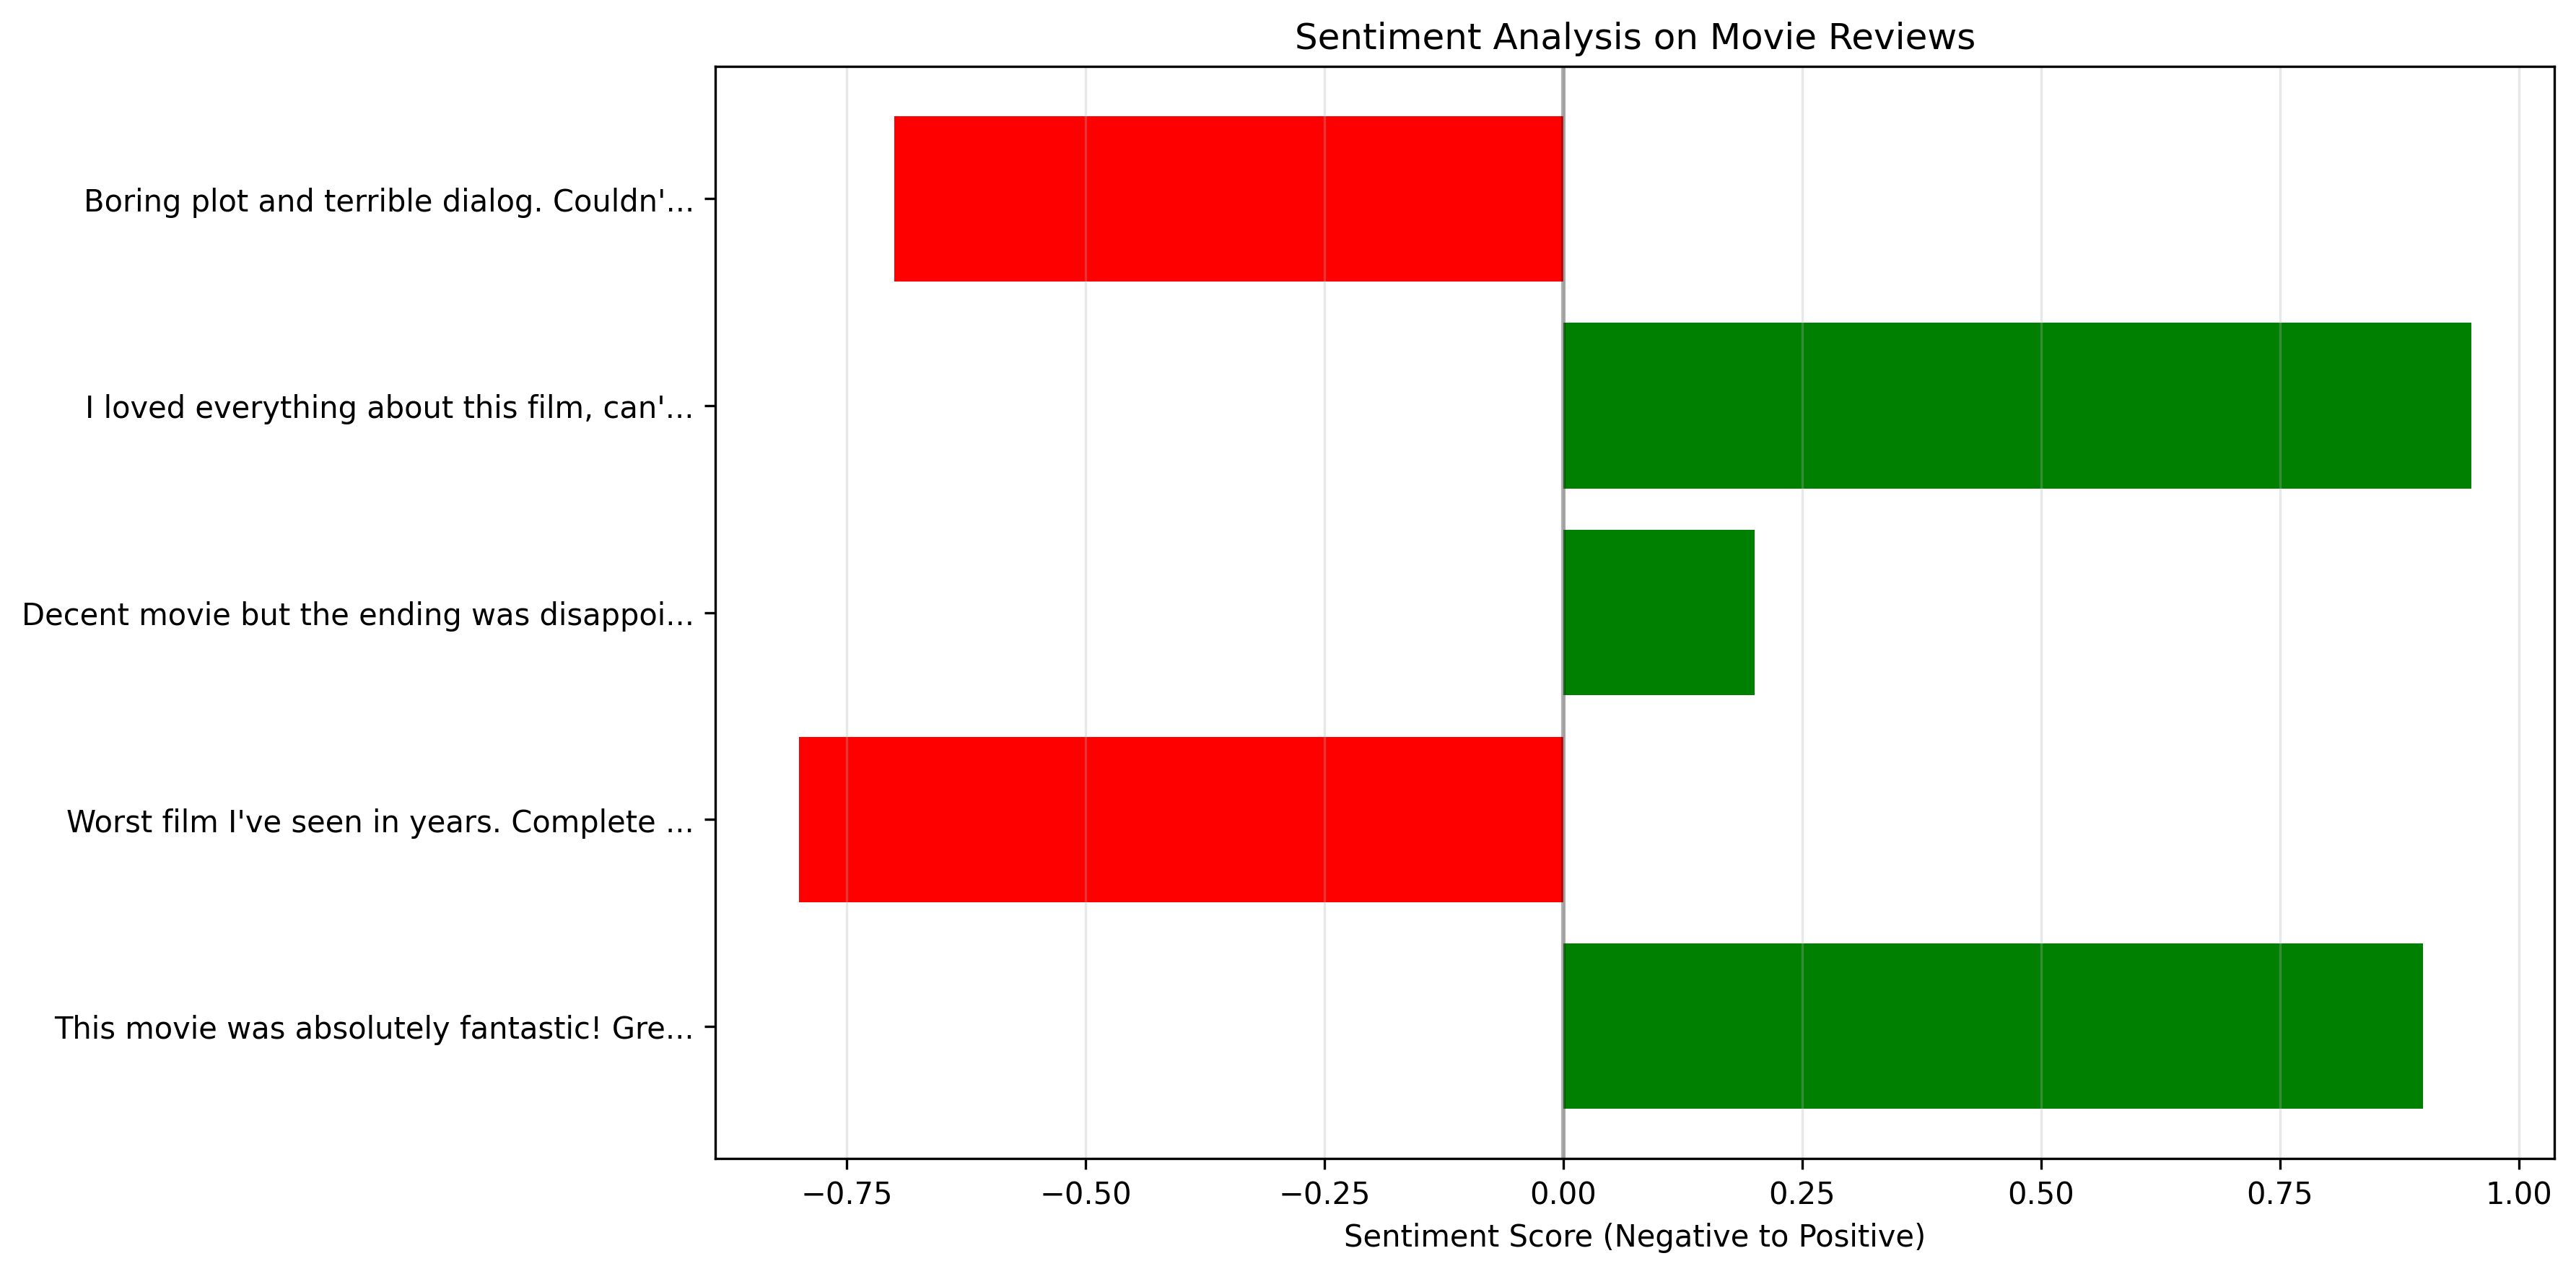
\includegraphics[width=\textwidth]{images/generated/sentiment_analysis.png}
            \vspace{0.5cm}
            \begin{center}
                \small{Exemple d'analyse de sentiment sur des critiques de films}
            \end{center}
        \end{column}
    \end{columns}
\end{frame}

% Third slide: Applications of NLP - Translation and Chatbots
\begin{frame}{Applications du NLP: Traduction et Assistants}
    \begin{columns}
        \begin{column}{0.5\textwidth}
            \textbf{Traduction automatique}
            \begin{itemize}
                \item Traduction instantanée entre langues
                \item Facilite la communication internationale
                \item Applications: Google Translate, DeepL
            \end{itemize}
            \vspace{0.3cm}
            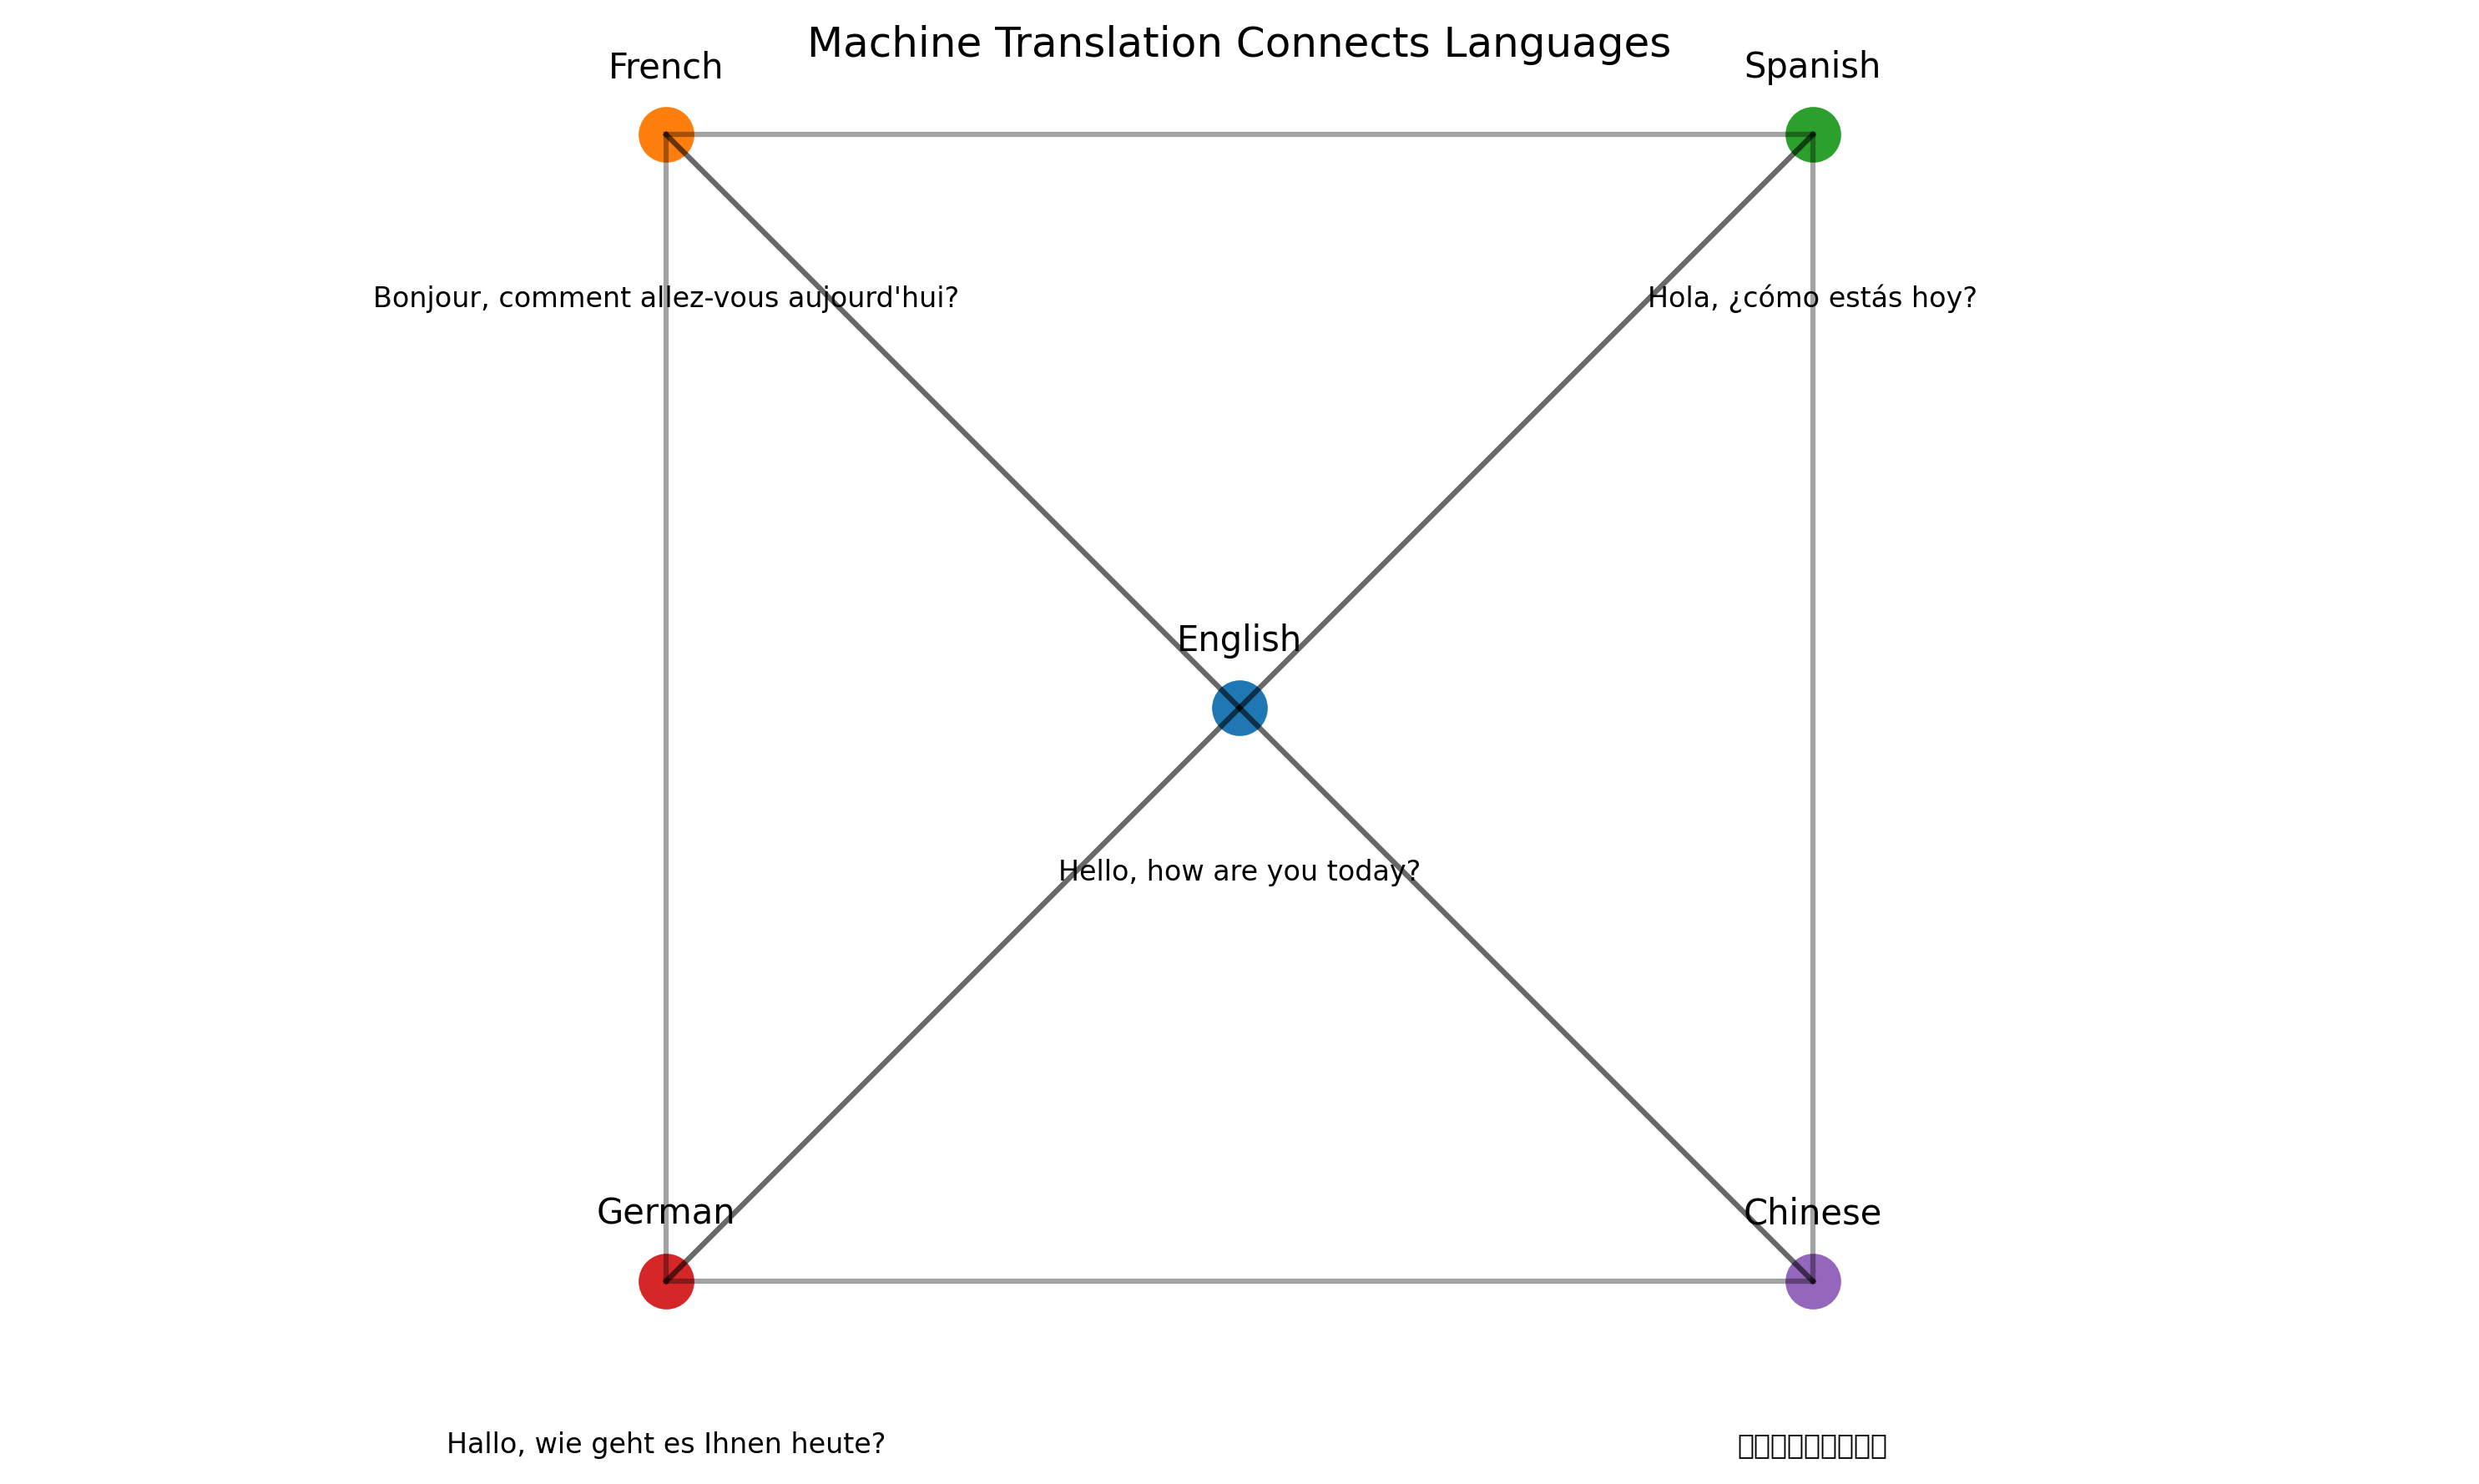
\includegraphics[width=\textwidth]{images/generated/translation.png}
        \end{column}
        \begin{column}{0.5\textwidth}
            \textbf{Chatbots et assistants virtuels}
            \begin{itemize}
                \item Répondent automatiquement aux questions
                \item Peuvent effectuer des tâches spécifiques
                \item Applications: assistants vocaux, service client
            \end{itemize}
            \vspace{0.3cm}
            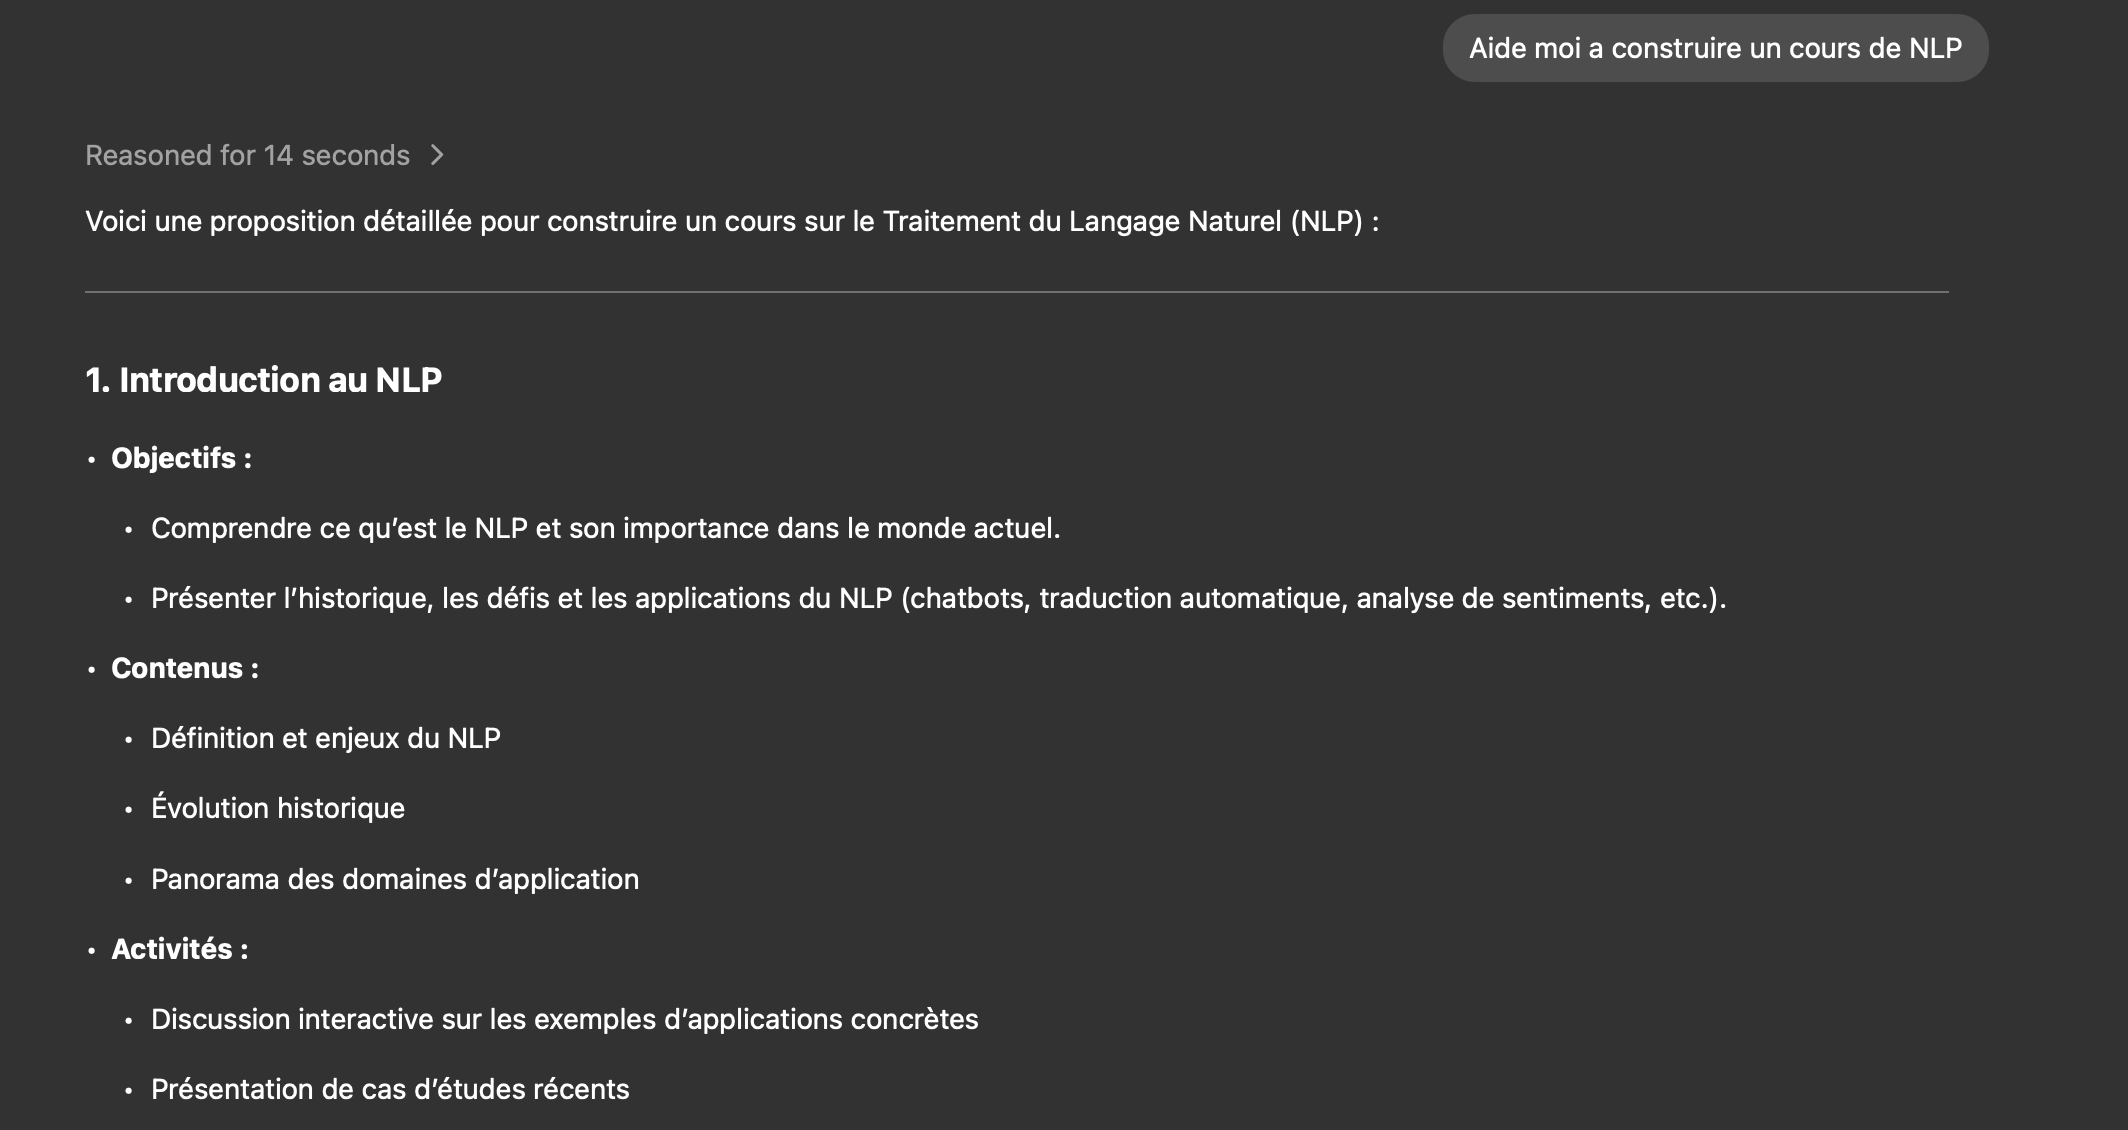
\includegraphics[width=\textwidth]{images/chatbot.png}
        \end{column}
    \end{columns}
\end{frame}

% New section on NLP basics and tokenization
\section{Bases du Traitement du Langage Naturel}

% Slide: What is a word in computing
\begin{frame}{Représentation des mots en informatique}
    \begin{itemize}
        \item En informatique, un \textbf{mot} est représenté comme une \textbf{séquence de caractères}
        \item Chaque \textbf{caractère} est encodé sur un nombre fini de bits:
        \begin{itemize}
            \item ASCII: 7 bits (128 caractères)
            \item Unicode: jusqu'à 32 bits (plus de 143 000 caractères)
        \end{itemize}
        \vspace{0.3cm}
        \item Pour traiter le langage, les modèles ont besoin de \textbf{représentations numériques}
        \item Le texte doit être converti en nombres pour être compris par les algorithmes
        \item Cette conversion s'appelle la \textbf{tokenisation}
    \end{itemize}
\end{frame}

% Slide: Different tokenization methods - Character tokenization
\begin{frame}{Encodage des caractères}
    \begin{columns}
        \begin{column}{0.55\textwidth}
            \begin{itemize}
                \item En informatique, chaque caractère a un \textbf{identifiant numérique unique}
                \begin{itemize}
                    \item Exemple simple: a=0, b=1, c=2, etc.
                    \item En réalité: tables d'encodage (ASCII, Unicode)
                \end{itemize}
                \vspace{0.1cm}
                \item \textbf{Tokenisation par caractère}:
                \begin{itemize}
                    \item Chaque caractère = un token
                    \item Vocabulaire très limité (128-256 tokens)
                    \item Séquences très longues
                \end{itemize}
                \vspace{0.1cm}
                \item \textbf{Avantages}:
                \begin{itemize}
                    \item Pas de mots inconnus
                    \item Solution universelle pour toutes les langues
                \end{itemize}
            \end{itemize}
        \end{column}
        \begin{column}{0.45\textwidth}
            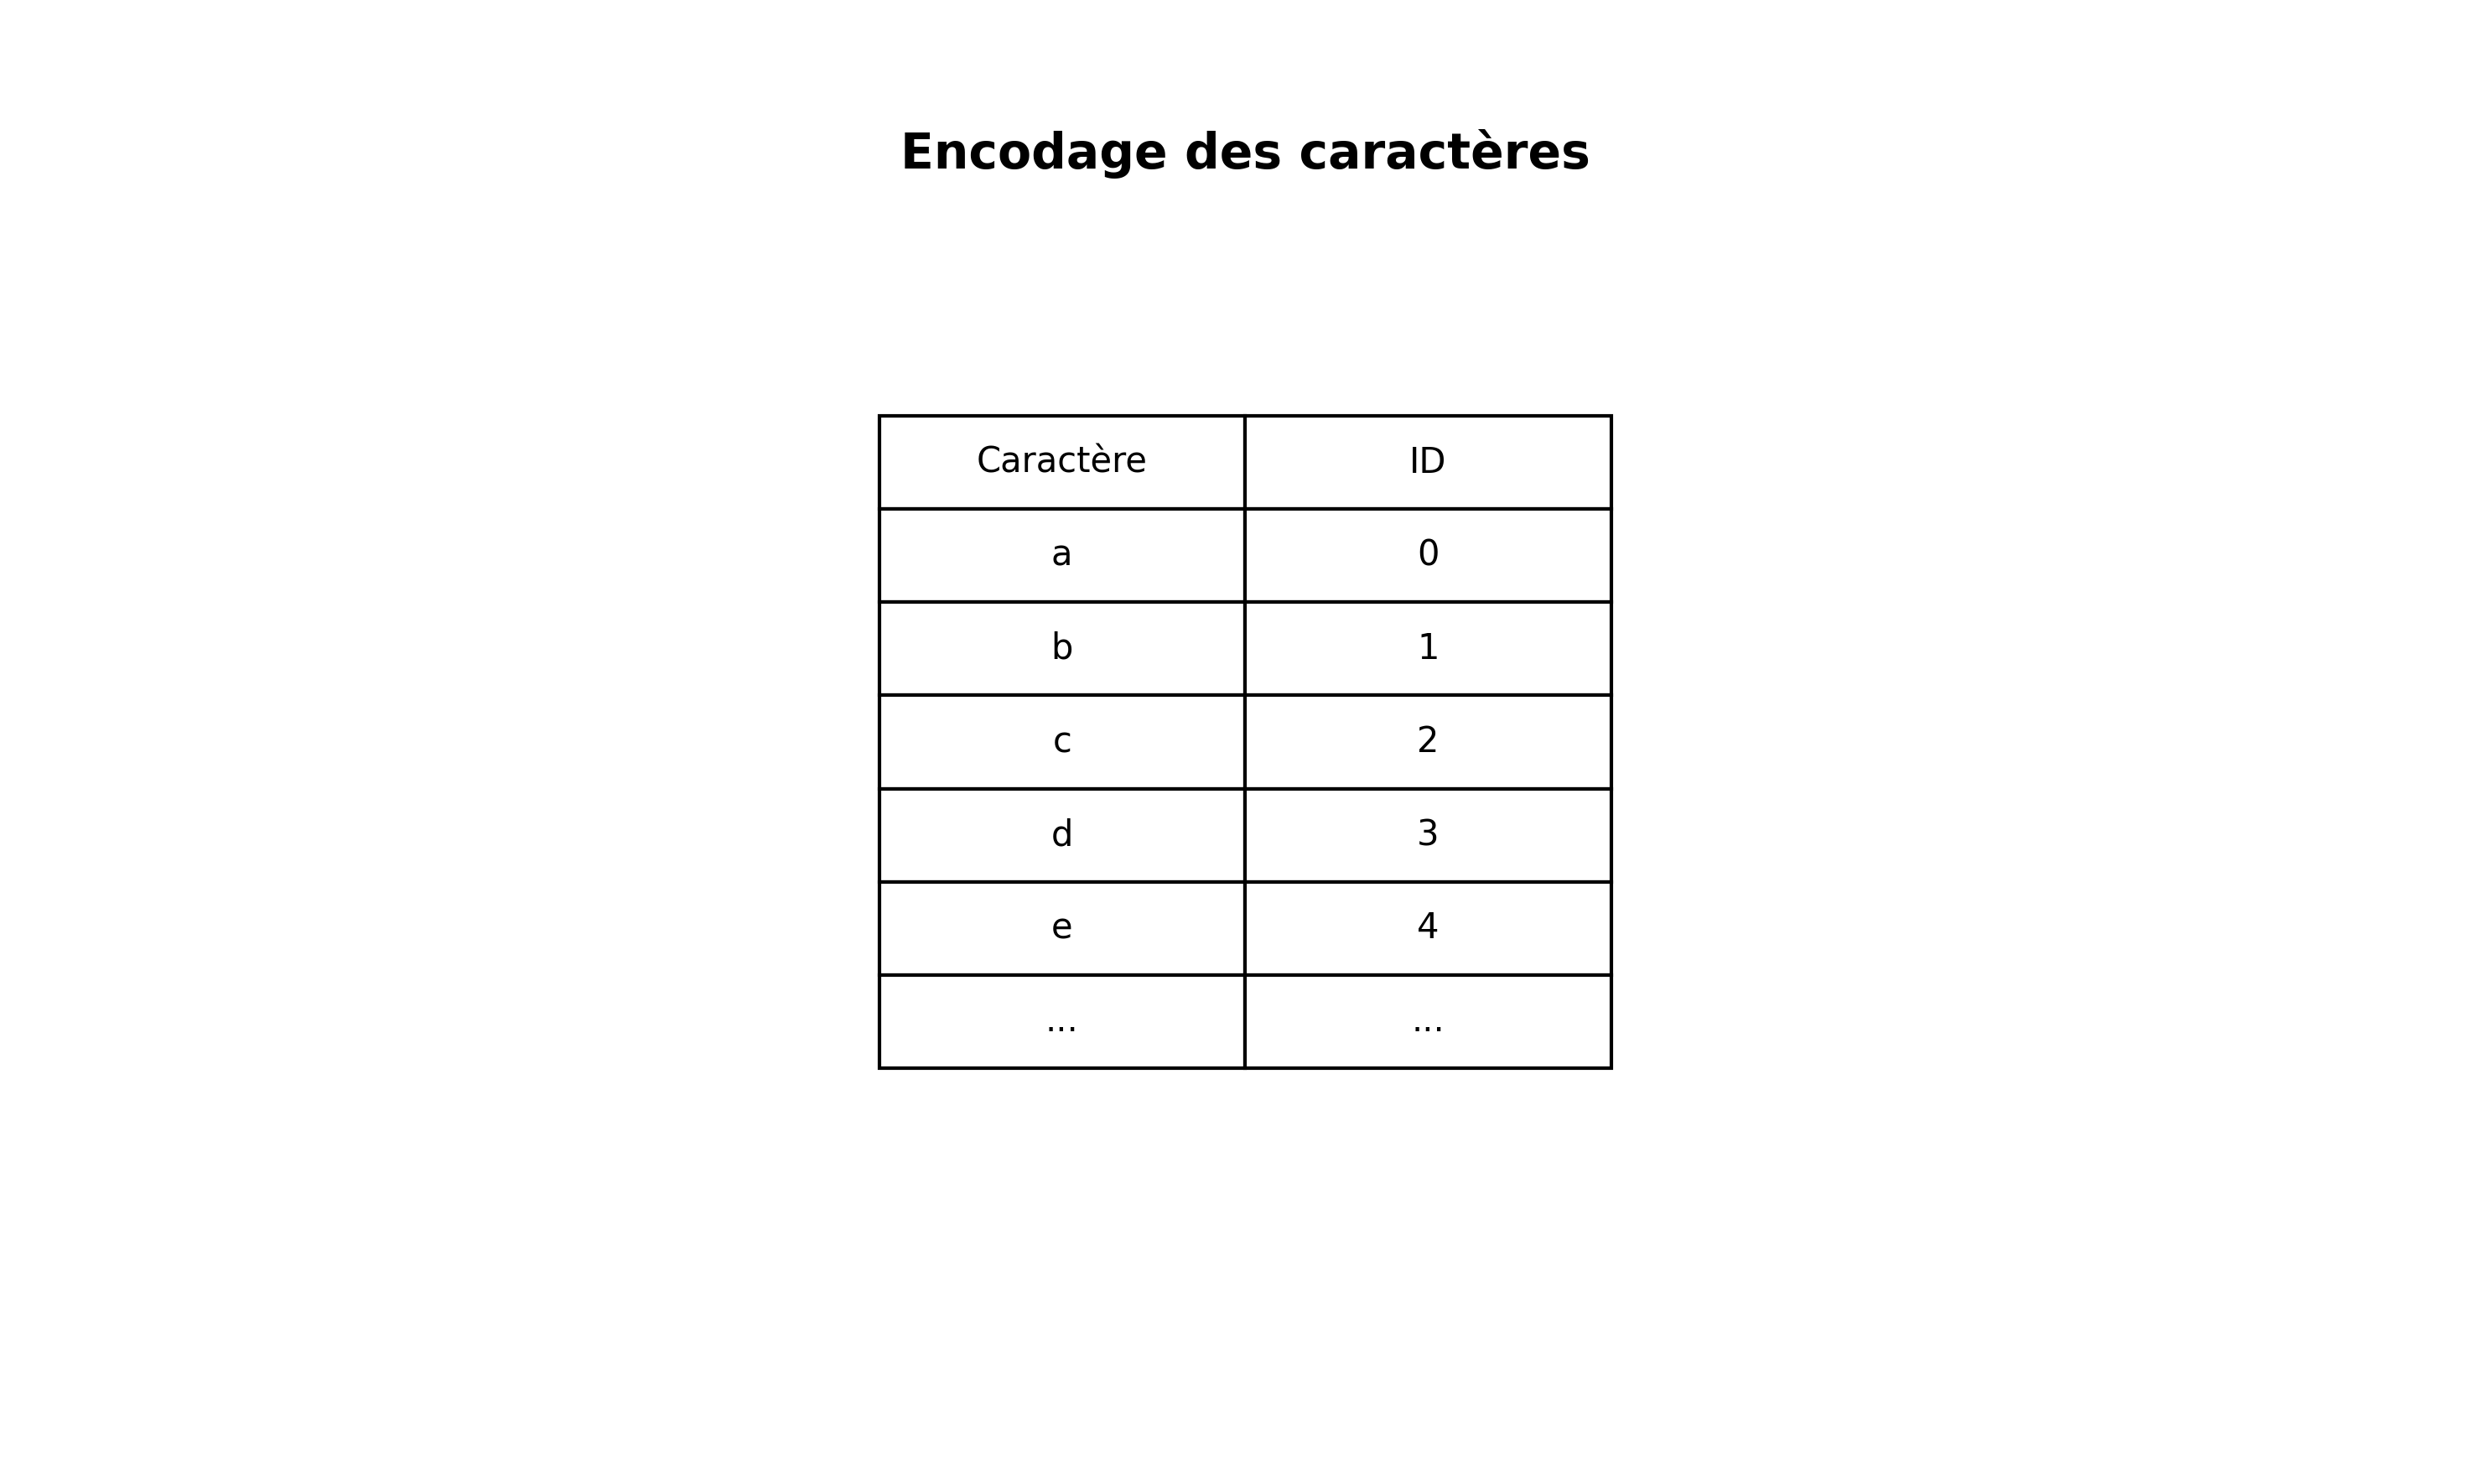
\includegraphics[width=0.95\textwidth]{images/generated/char_tokenization.png}
            \vspace{0.1cm}
            \begin{center}
                \small{Correspondance entre caractères et identifiants}
            \end{center}
        \end{column}
    \end{columns}
\end{frame}

% Slide: Different tokenization methods - Word and subword tokenization
\begin{frame}{Méthodes de tokenisation 2: Mots et sous-mots}
    \begin{columns}
        \begin{column}{0.5\textwidth}
            \begin{itemize}
                \item \textbf{Tokenisation par mot}:
                \begin{itemize}
                    \item Chaque mot = un token
                    \item Vocabulaire très grand (100K-1M tokens)
                    \item Problème des mots inconnus (OOV)
                    \item Difficulté avec les variations morphologiques
                \end{itemize}
                \vspace{0.3cm}
                \item \textbf{Tokenisation par sous-mots}:
                \begin{itemize}
                    \item Compromis entre caractères et mots
                    \item Vocabulaire raisonnable (10K-50K tokens)
                    \item Capture les morphèmes et parties de mots
                    \item Solution privilégiée par les modèles actuels
                \end{itemize}
            \end{itemize}
        \end{column}
        \begin{column}{0.5\textwidth}
            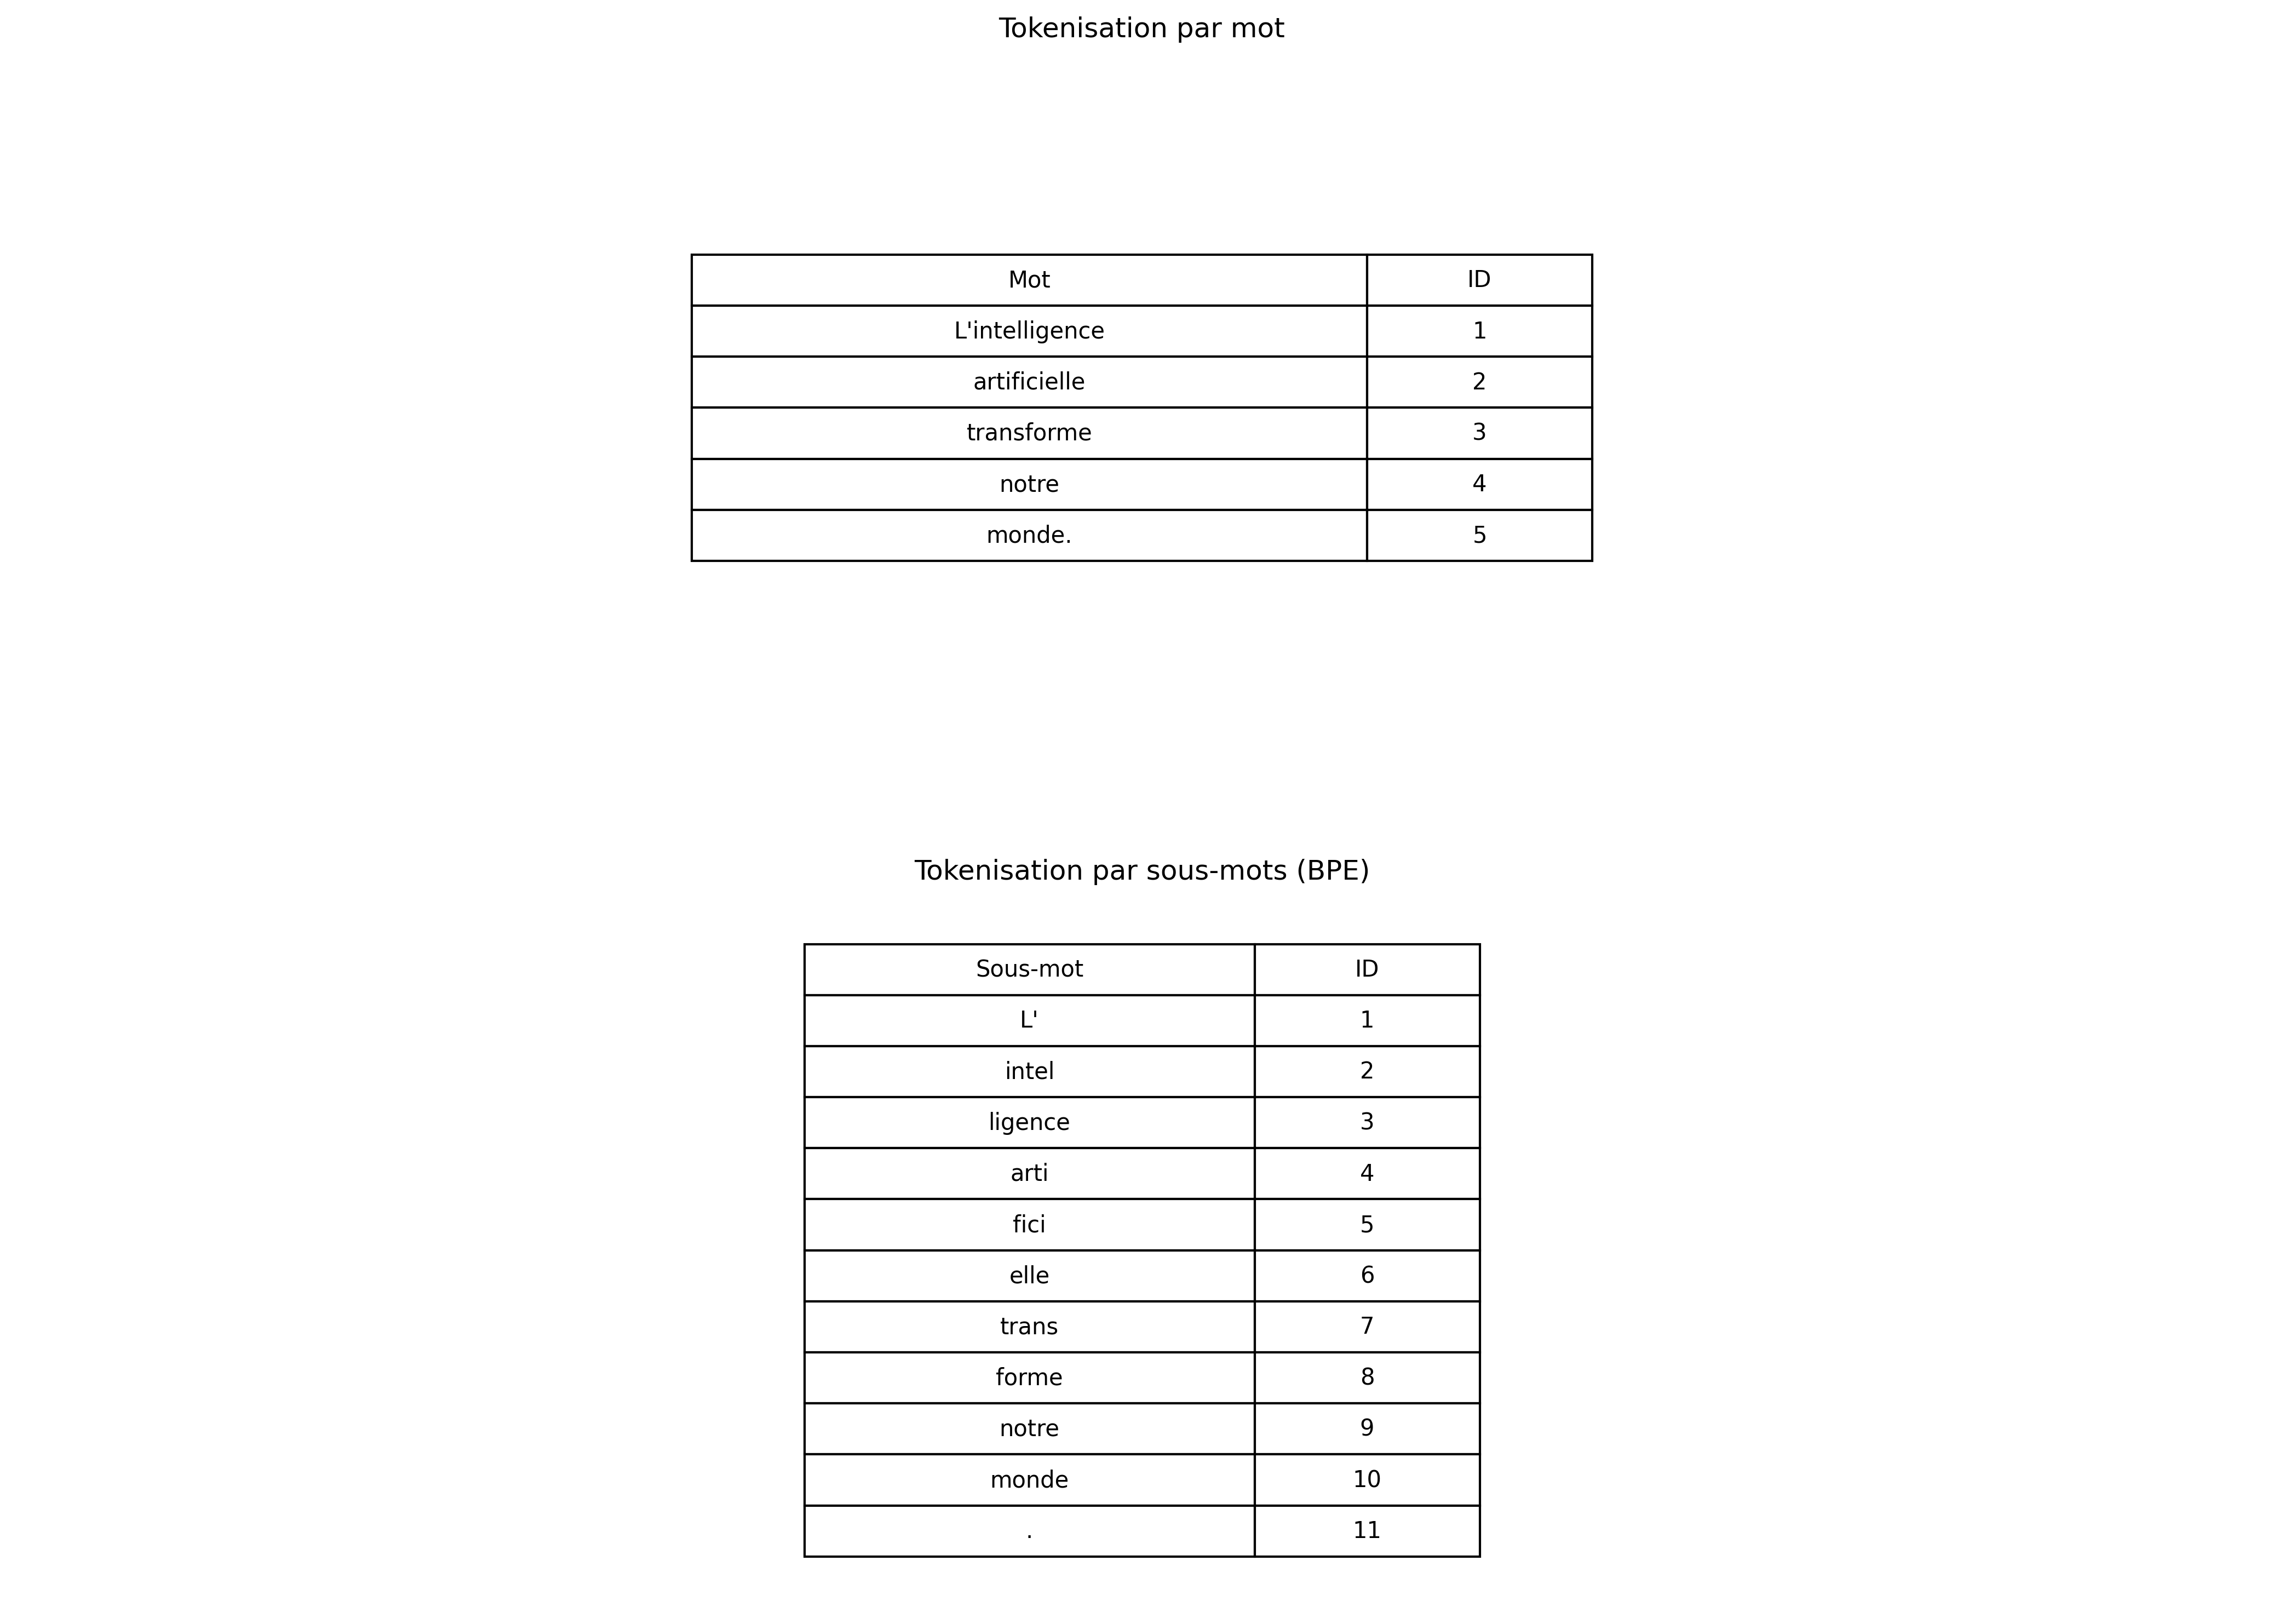
\includegraphics[width=\textwidth]{images/generated/word_subword_tokenization.png}
            \vspace{0.2cm}
            \begin{center}
                \small{Tokenisations par mot et sous-mot de la phrase d'exemple}
            \end{center}
        \end{column}
    \end{columns}
\end{frame}

% Slide: Vocabulary size comparison
\begin{frame}{Comparaison des tailles de vocabulaire}
    \begin{columns}
        \begin{column}{0.5\textwidth}
            \textbf{Compromis entre taille et expressivité}:
            \begin{itemize}
                \item \textbf{Vocabulaire petit} (caractères):
                \begin{itemize}
                    \item Avantage: pas de mots inconnus
                    \item Inconvénient: séquences très longues
                \end{itemize}
                \vspace{0.3cm}
                \item \textbf{Vocabulaire grand} (mots):
                \begin{itemize}
                    \item Avantage: capture directement les unités sémantiques
                    \item Inconvénient: nombreux mots inconnus
                \end{itemize}
                \vspace{0.3cm}
                \item \textbf{Vocabulaire intermédiaire} (sous-mots):
                \begin{itemize}
                    \item Équilibre entre les deux approches
                    \item Solution adoptée par la plupart des modèles modernes
                \end{itemize}
            \end{itemize}
        \end{column}
        \begin{column}{0.5\textwidth}
            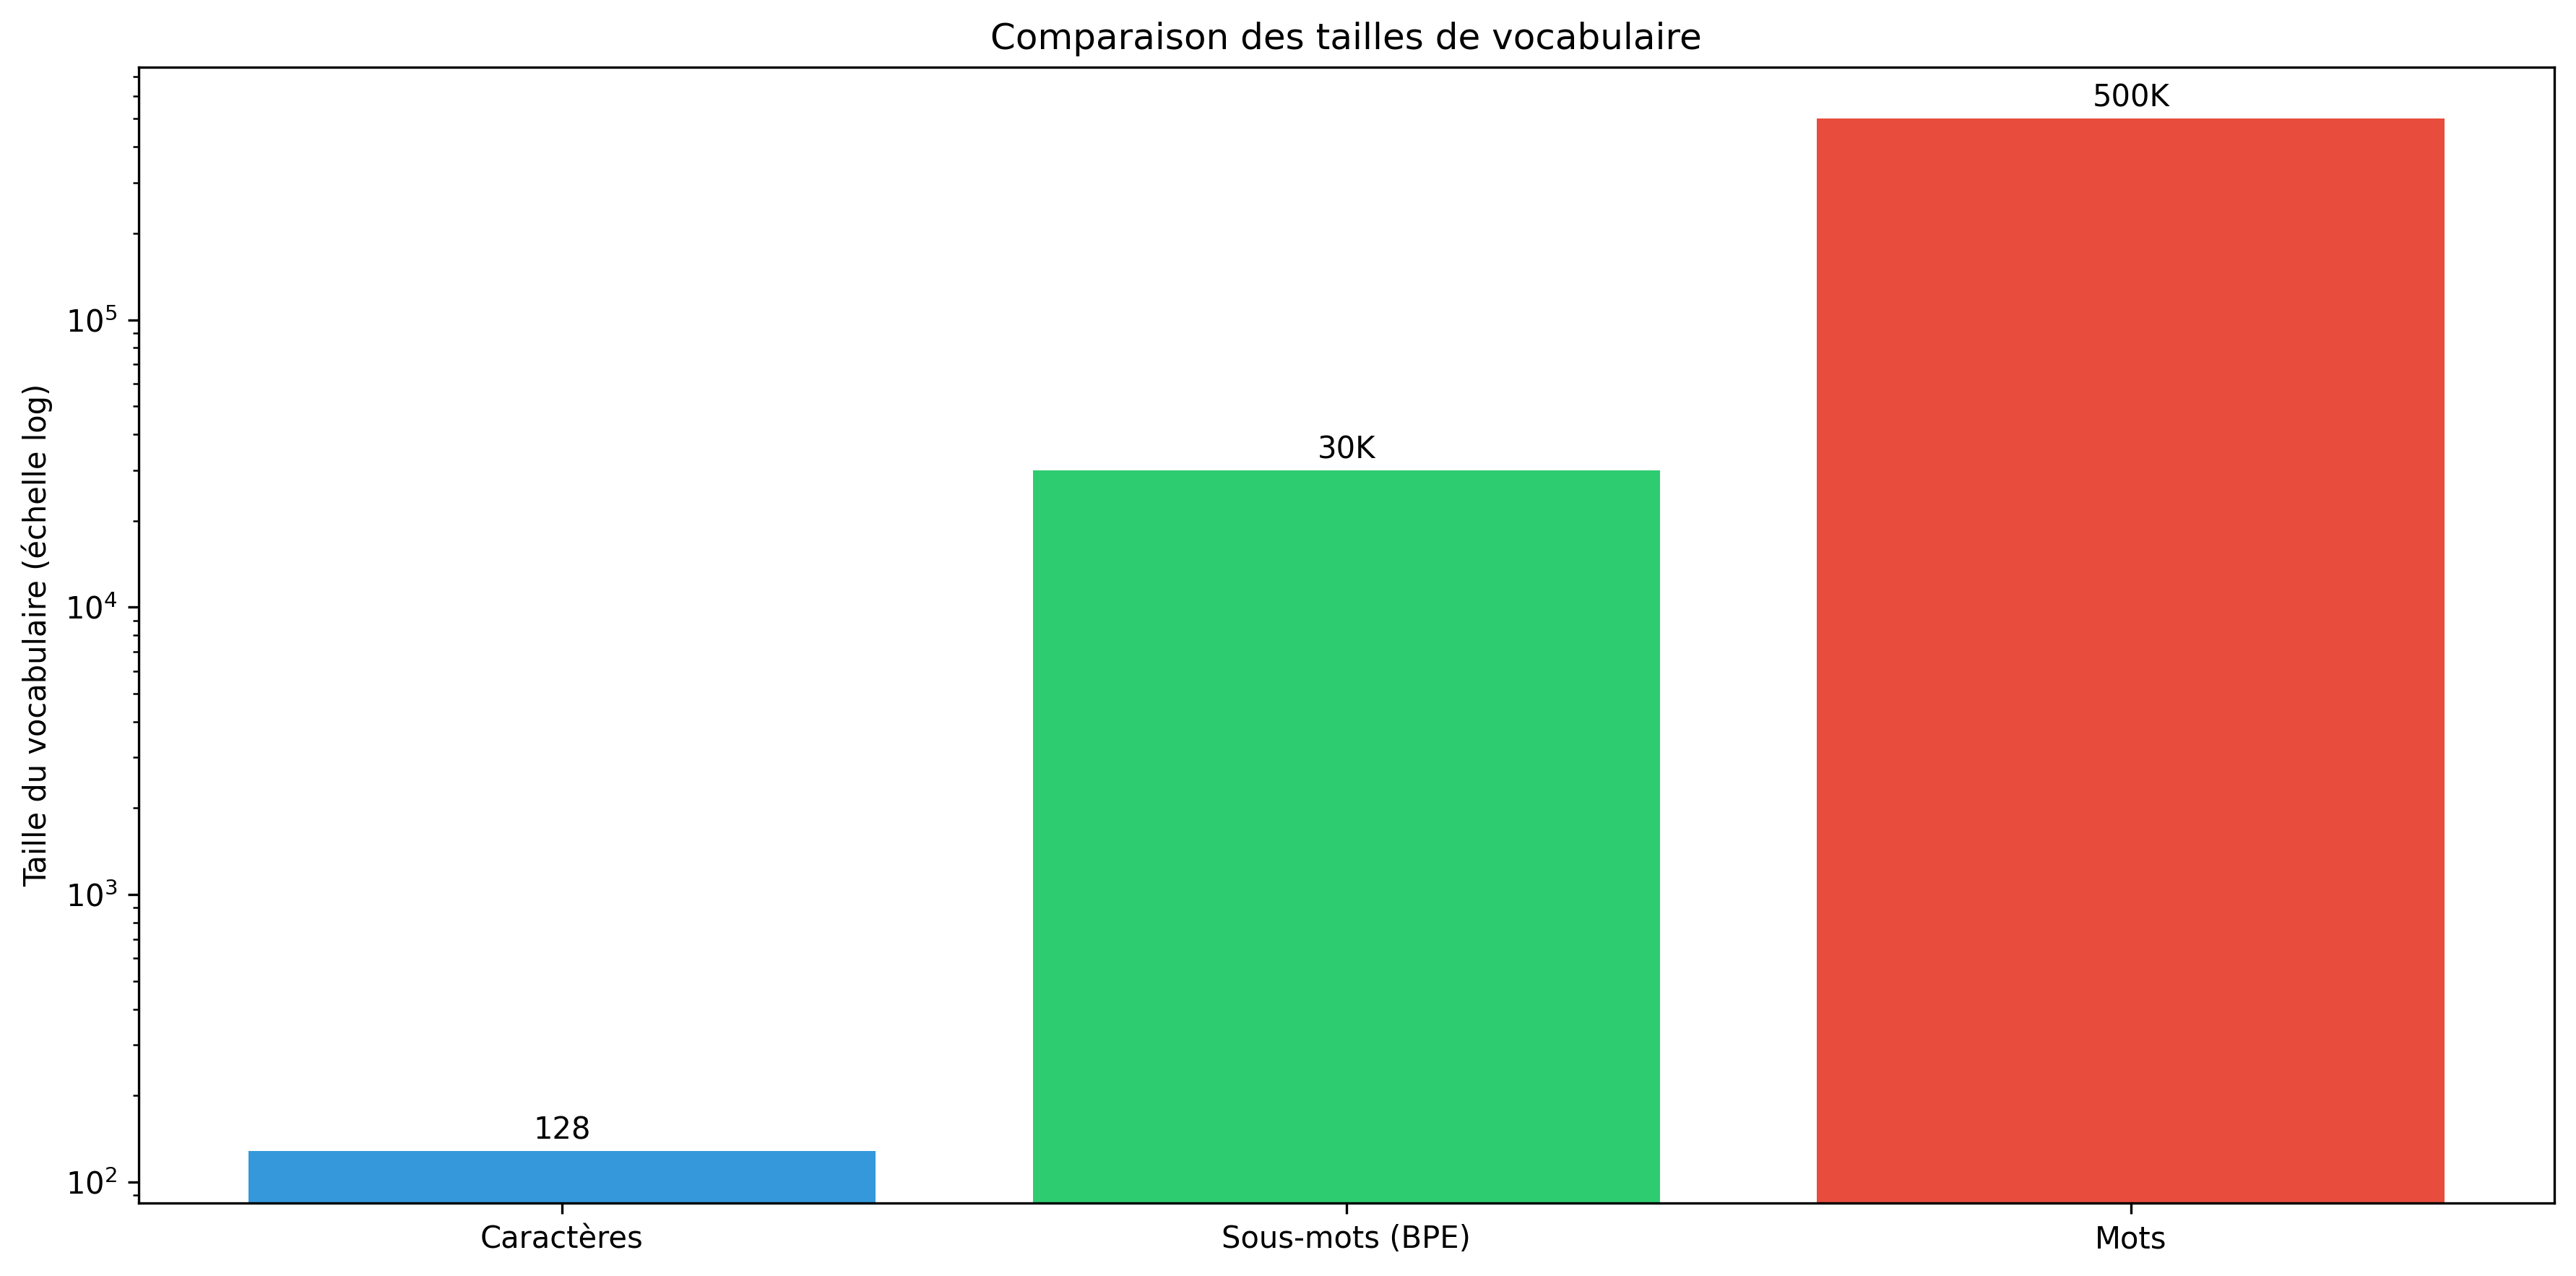
\includegraphics[width=\textwidth]{images/generated/vocab_size_comparison.png}
            \vspace{0.2cm}
            \begin{center}
                \small{Comparaison des tailles de vocabulaire selon la méthode}
            \end{center}
        \end{column}
    \end{columns}
\end{frame}

% Slide: BPE Algorithm
\begin{frame}{Algorithme BPE (Byte Pair Encoding)}
    \begin{columns}
        \begin{column}{0.45\textwidth}
            \textbf{Principe du BPE}:
            \begin{enumerate}
                \item Commencer avec un vocabulaire de caractères
                \item Identifier les paires de tokens les plus fréquentes
                \item Fusionner ces paires pour créer un nouveau token
                \item Répéter jusqu'à atteindre la taille de vocabulaire souhaitée
            \end{enumerate}
            \vspace{0.3cm}
            \textbf{Avantages}:
            \begin{itemize}
                \item Adapté au corpus d'entraînement
                \item Gère efficacement les mots rares
                \item Capture les morphèmes et affixes
                \item Utilisé dans GPT, BERT, T5, etc.
            \end{itemize}
        \end{column}
        \begin{column}{0.55\textwidth}
            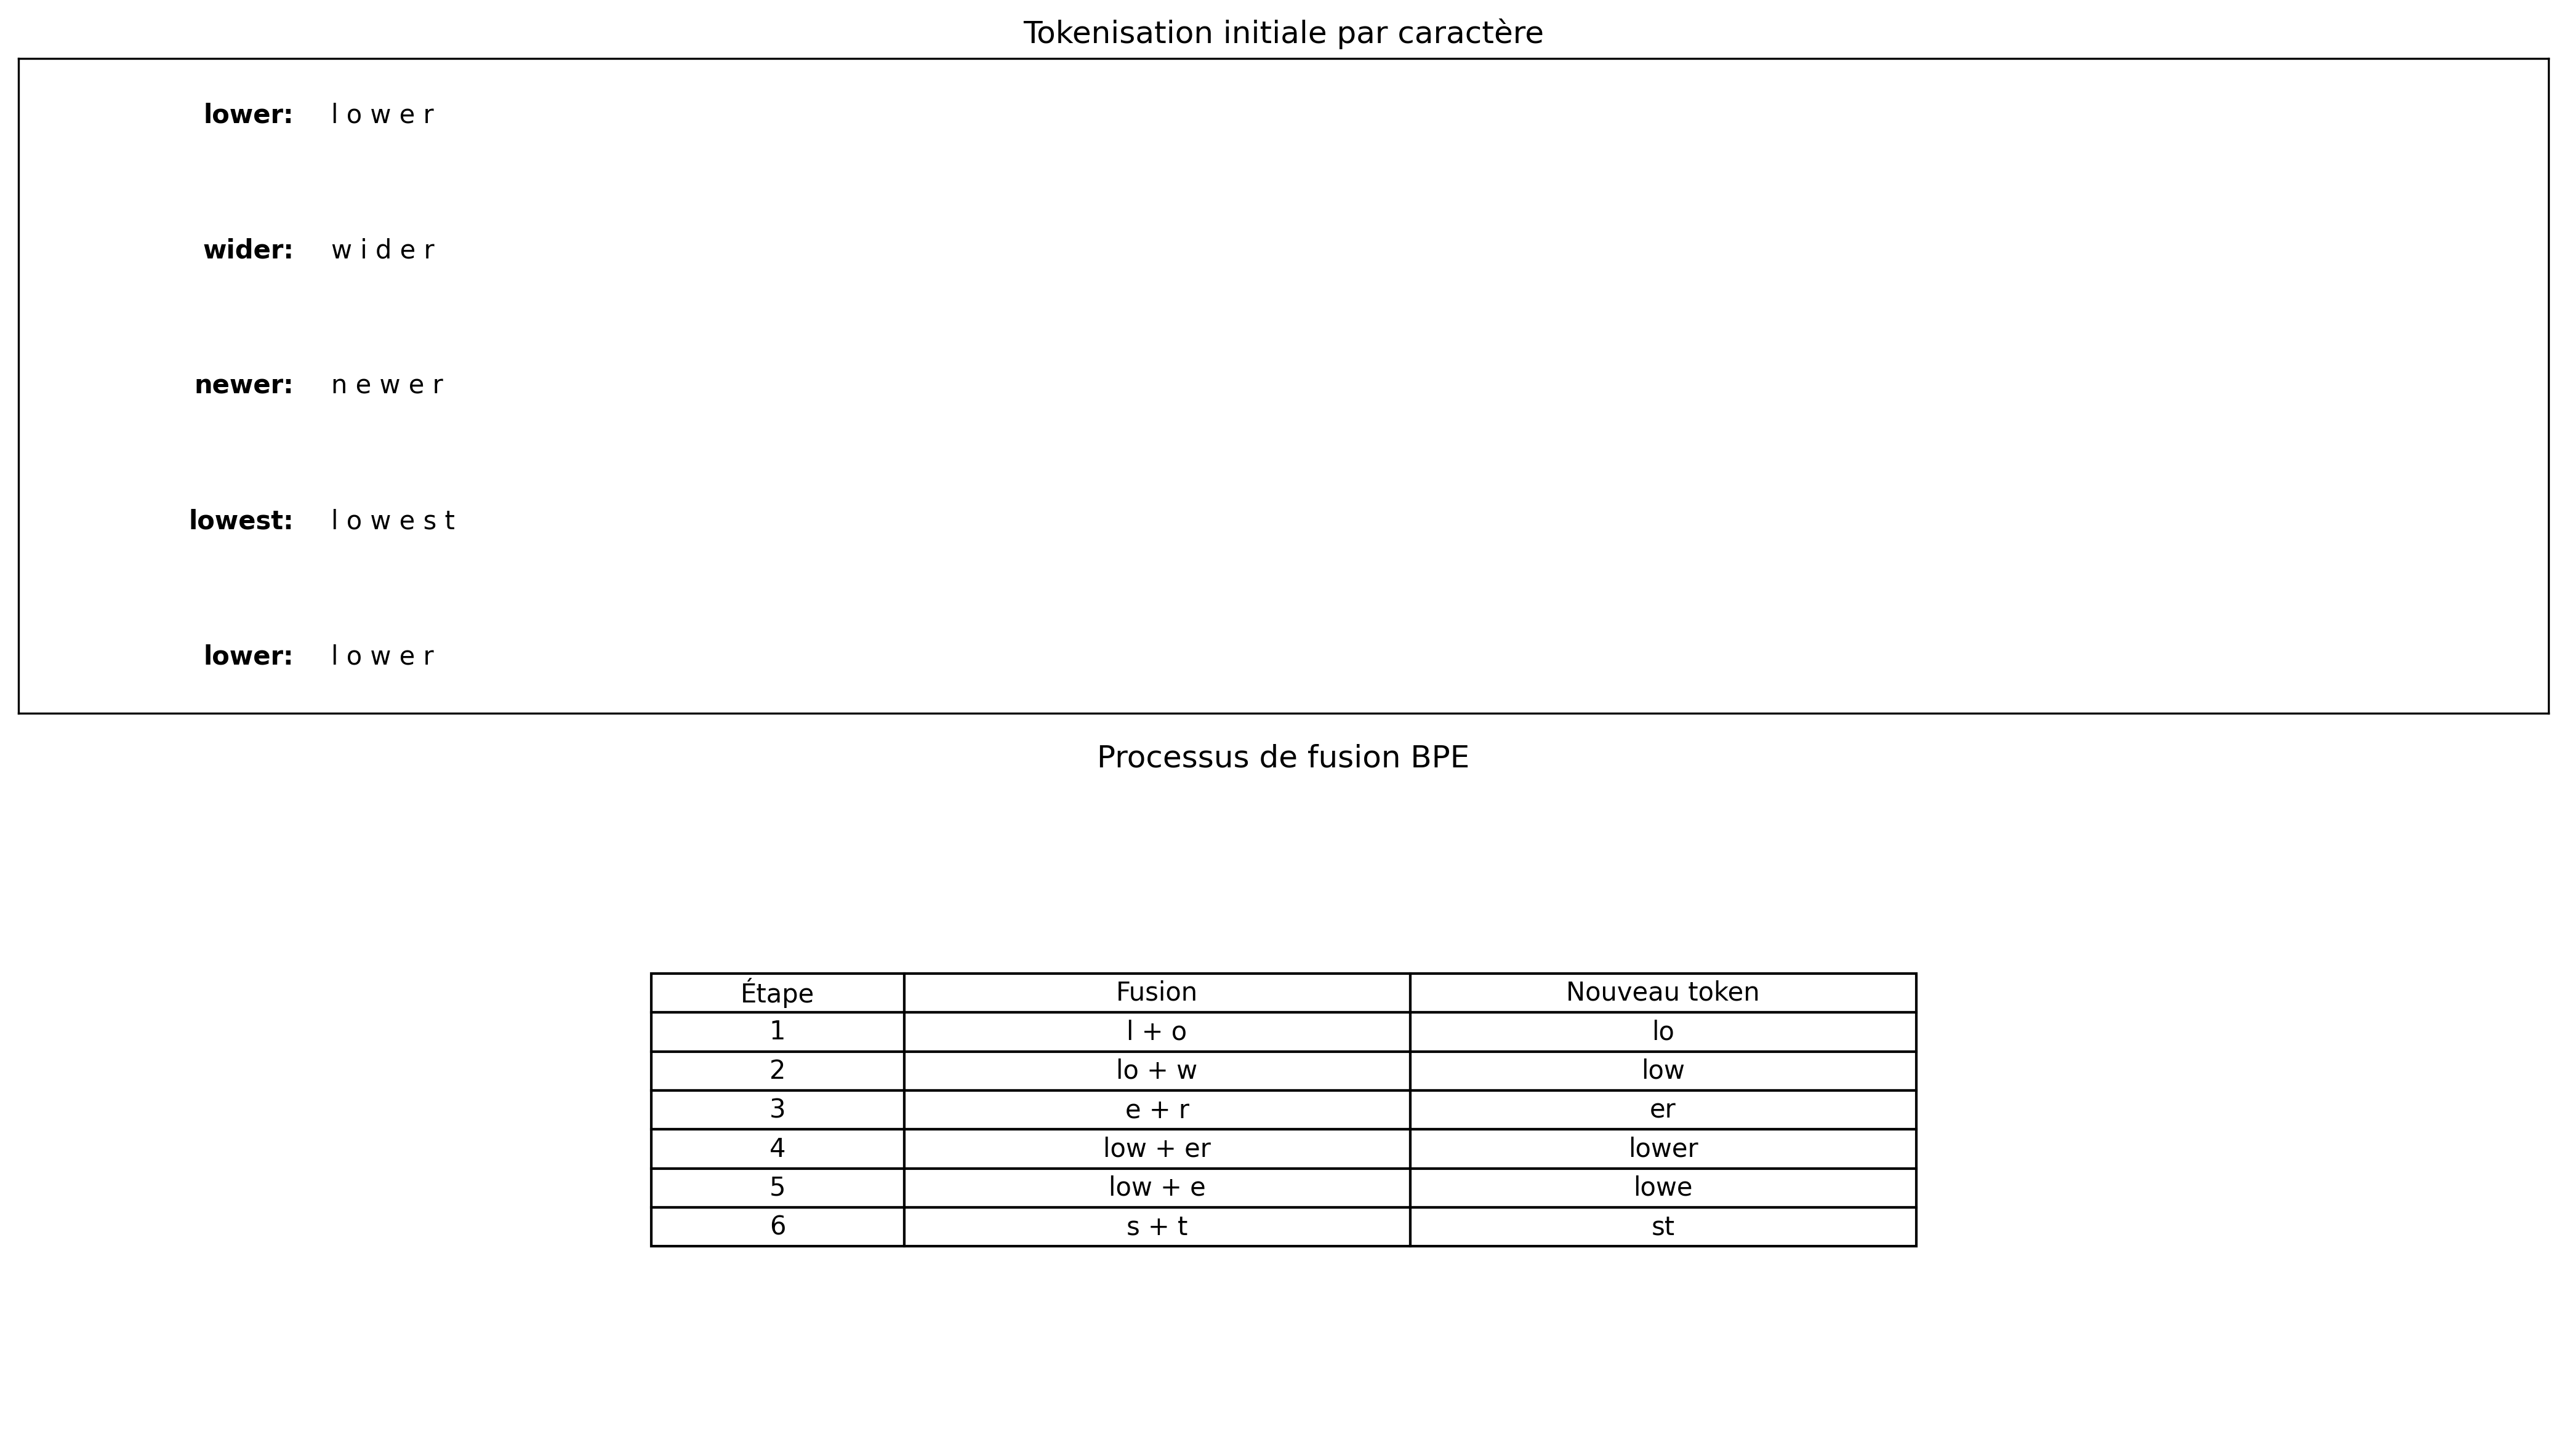
\includegraphics[width=\textwidth]{images/generated/bpe_algorithm.png}
            \vspace{0.2cm}
            \begin{center}
                \small{Exemple de fusion progressive avec BPE}
            \end{center}
        \end{column}
    \end{columns}
\end{frame}

\begin{frame}{Démonstration: Tokenisation en pratique}
    \begin{center}
        Démonstration sur Jupyter Notebook
    \end{center}
\end{frame}


\begin{frame}
    \frametitle{Tokenizers: Un composant distinct du modèle}
    
    \begin{columns}[T]
        \begin{column}{0.45\textwidth}
            \begin{itemize}
                \item Un même modèle peut utiliser différents tokenizers
                \item Un même tokenizer peut être utilisé par de multiples modèles
                \item Le choix du tokenizer influence directement les performances du modèle
            \end{itemize}
        \end{column}
        
        \begin{column}{0.55\textwidth}
            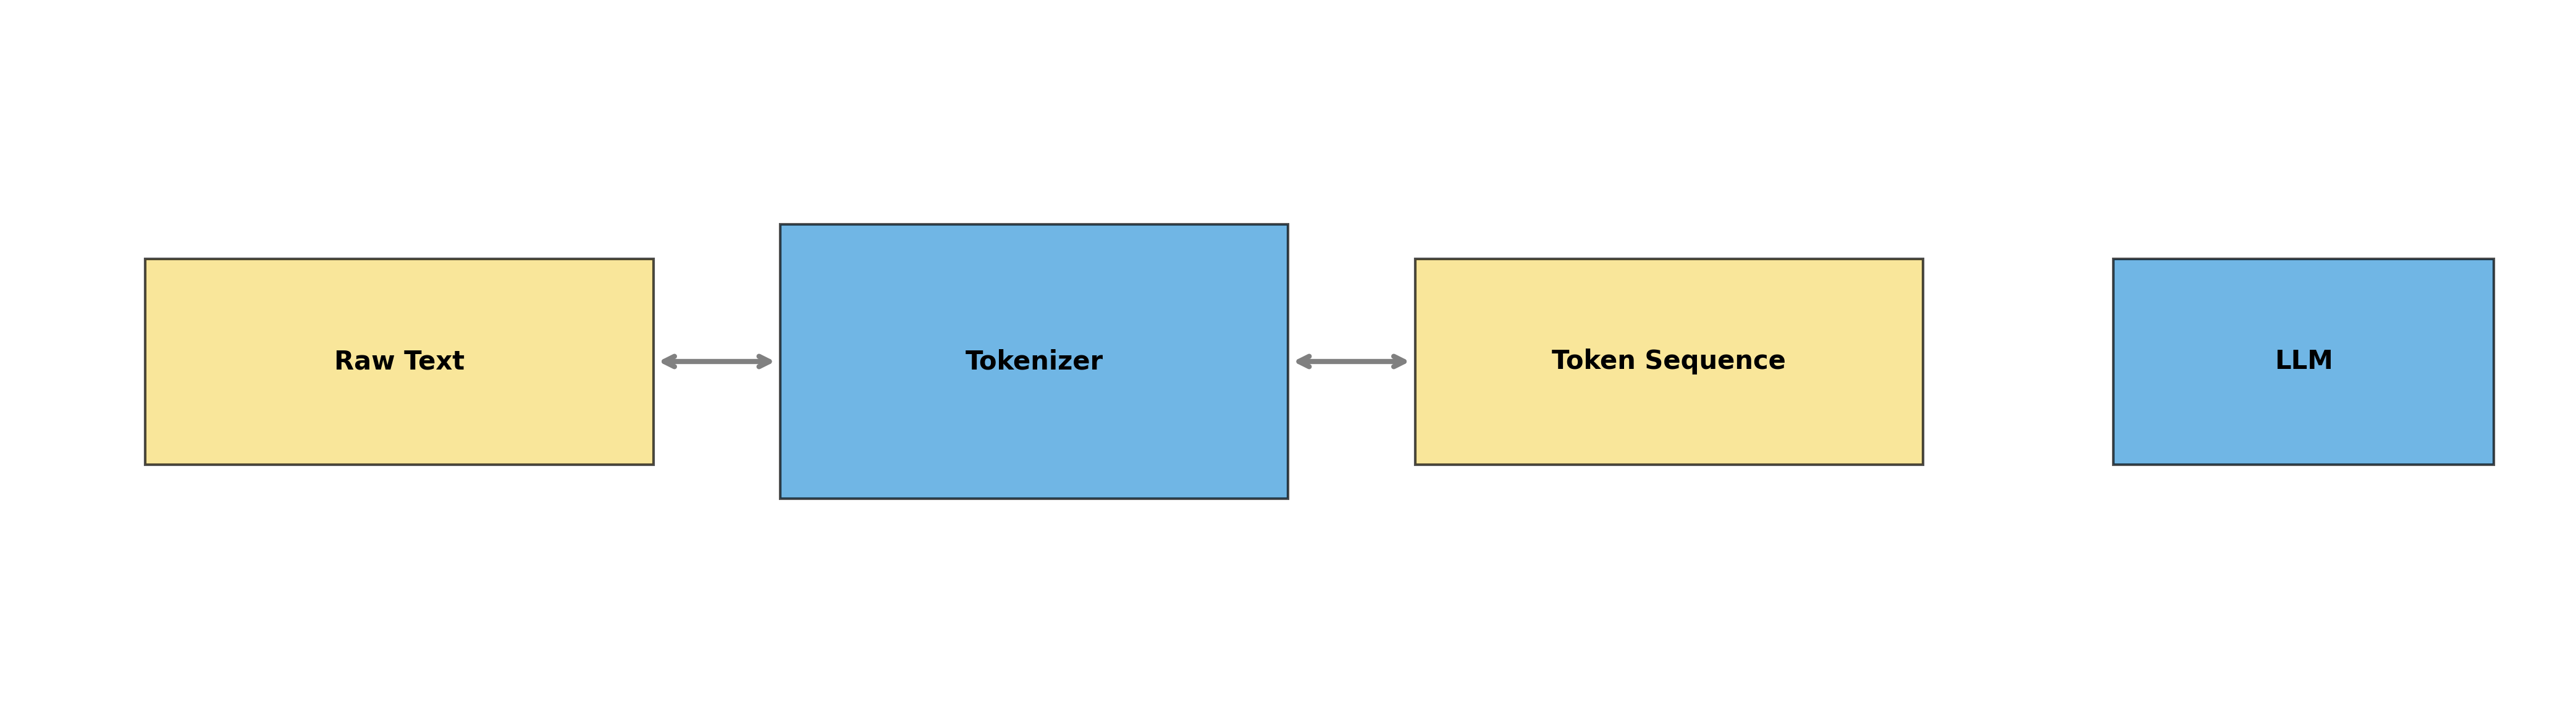
\includegraphics[width=\textwidth]{images/generated/tokenizer_model_separation.png}
            \vspace{-0.5cm}
            \begin{center}
                \footnotesize{Le tokenizer est la passerelle entre le langage humain et le langage machine}
            \end{center}
        \end{column}
    \end{columns}
    
    \vspace{0.3cm}
    \begin{alertblock}{Points clés}
        Le tokenizer est une étape de prétraitement \textbf{cruciale} et \textbf{indépendante} qui conditionne la qualité des représentations du langage dans tous les modèles de NLP.
    \end{alertblock}
\end{frame}

\begin{frame}
    \frametitle{Au-delà du BPE: Une diversité d'approches pour la tokenisation}
    
    \begin{columns}[T]
        \begin{column}{0.5\textwidth}
            \textbf{Alternatives au BPE:}
            \begin{itemize}
                \item \textbf{WordPiece} (Google, BERT)
                \begin{itemize}
                    \item Fusion basée sur la probabilité des paires
                    \item Optimisation de la vraisemblance du corpus
                \end{itemize}
                \vspace{0.2cm}
                \item \textbf{Unigram Language Model} (SentencePiece)
                \begin{itemize}
                    \item Approche probabiliste (EM algorithm)
                    \item Permet plusieurs segmentations possibles
                \end{itemize}
                \vspace{0.2cm}
                \item \textbf{Byte-level BPE} (GPT-2, RoBERTa)
                \begin{itemize}
                    \item Opère sur les bytes plutôt que les caractères
                    \item Vocabulaire universel garanti
                \end{itemize}
            \end{itemize}
        \end{column}
        
        \begin{column}{0.5\textwidth}
            \textbf{Tokenizers spécialisés:}
            \begin{itemize}
                \item \textbf{CharacterBERT}: Modèle basé sur les caractères
                \item \textbf{SentencePiece}: Solution pour langues non-segmentées (japonais, chinois)
                \item \textbf{CANINE}: Tokenizer-free architecture
            \end{itemize}
        \end{column}
    \end{columns}
\end{frame}

\begin{frame}
    \frametitle{Tokens Spéciaux: Au-delà des Mots et Sous-mots}
    
    \begin{columns}[T]
        \begin{column}{0.5\textwidth}
            \textbf{Tokens de contrôle et structure:}
            \begin{itemize}
                \item \textbf{Début/Fin}:
                \begin{itemize}
                    \item \texttt{<|endoftext|>} (GPT)
                    \item \texttt{<s>}, \texttt{</s>} (RoBERTa)
                \end{itemize}
                \vspace{0.1cm}
                \item \textbf{Traitement de séquence}:
                \begin{itemize}
                    \item \texttt{<pad>} (padding)
                    \item \texttt{<unk>} (token inconnu)
                    \item \texttt{<mask>} (pour masked language modeling)
                \end{itemize}
                \vspace{0.1cm}
                \item \textbf{Dialogue et conversation}:
                \begin{itemize}
                    \item \texttt{<|im\_start|>}, \texttt{<|im\_end|>} (ChatGPT)
                    \item \texttt{<human>}, \texttt{<assistant>} (Claude)
                \end{itemize}
                \vspace{0.1cm}
                \item \textbf{Raisonnement}:
                \begin{itemize}
                    \item \texttt{<think>}, \texttt{</think>}
                    \item \texttt{<reasoning>}, \texttt{</reasoning>}
                \end{itemize}
            \end{itemize}
        \end{column}
        
        \begin{column}{0.5\textwidth}
            \textbf{Tokens pour contenus spécifiques:}
            \begin{itemize}
                \item \textbf{Programmation}:
                \begin{itemize}
                    \item \texttt{<code>}, \texttt{</code>}
                    \item \texttt{<python>}, \texttt{<json>}, etc.
                \end{itemize}
                \vspace{0.2cm}
            \end{itemize}
            
            \begin{alertblock}{Importance des tokens spéciaux}
                Les tokens spéciaux permettent de:
                \begin{itemize}
                    \item Structurer l'information pour le modèle
                    \item Contrôler le comportement de génération
                    \item Améliorer les performances sur des tâches spécifiques
                    \item Communiquer des instructions implicites au modèle
                \end{itemize}
            \end{alertblock}
        \end{column}
    \end{columns}
\end{frame}

% Nouvelle section sur la Classification de Sentiment
\section{Classification de Sentiment: Approches Traditionnelles}

% Slide: Introduction à la classification de sentiment
\begin{frame}{Introduction à la Classification de Sentiment}
    \begin{itemize}
        \item La \textbf{classification de sentiment} est l'une des applications les plus courantes du NLP
        \item Elle vise à déterminer l'\textbf{opinion} ou l'\textbf{émotion} exprimée dans un texte
        \item Applications:
        \begin{itemize}
            \item Analyse des avis clients et commentaires sur les produits
            \item Surveillance de la réputation de marque sur les réseaux sociaux
            \item Étude de la réception d'événements ou de décisions politiques
            \item Prédiction des tendances de marché basées sur l'opinion publique
        \end{itemize}
        \item Différents niveaux de granularité:
        \begin{itemize}
            \item \textbf{Binaire}: positif vs. négatif
            \item \textbf{Multi-classe}: positif, neutre, négatif, etc.
            \item \textbf{Analyse fine}: détection de nuances, sarcasme, ironie
            \item \textbf{Analyse par aspect}: sentiment envers différents aspects d'un produit
        \end{itemize}
    \end{itemize}
\end{frame}

% Slide: Examples of IMDB reviews for sentiment classification
\begin{frame}{Exemples de critiques cinéma - Classification de sentiment}
    Comment classifieriez-vous le sentiment de ces critiques de films?
    
    \begin{exampleblock}{Critique 1}
        \small{A rating of ""1"" does not begin to express how dull, depressing and relentlessly bad this movie is.}
    \end{exampleblock}
    
    \begin{exampleblock}{Critique 2}
        \small{My kids picked this out at the video store...it's great to hear Liza as Dorothy cause she sounds just like her mom. But there are too many bad songs, and the animation is pretty crude compared to other cartoons of that time.}
    \end{exampleblock}
    
    \begin{exampleblock}{Critique 3}
        \small{Malcolm McDowell has not had too many good movies lately and this is no different. Especially designed for people who like Yellow filters on their movies.}
    \end{exampleblock}
    
    \vspace{0.3cm}
    \centering
\end{frame}

% Slide: Méthode Bag of Words
\begin{frame}{Bag of Words: Représentation Simplifiée du Texte}
    \begin{columns}
        \begin{column}{0.55\textwidth}
            \textbf{Principe du Bag of Words (BoW)}
            \begin{itemize}
                \item Représentation simple du texte comme un "sac de mots"
                \item \textbf{L'ordre des mots} est ignoré, seule la \textbf{fréquence} compte
                \item Chaque document devient un vecteur dans l'espace des mots
                \item Algorithme:
                \begin{enumerate}
                    \item Créer un \textbf{vocabulaire} de tous les mots uniques
                    \item Pour chaque document, compter les occurrences de chaque mot
                    \item Obtenir un vecteur de fréquences par document
                \end{enumerate}
                \item Application: recherche d'information, classification de texte, etc.
            \end{itemize}
        \end{column}
        \begin{column}{0.45\textwidth}
            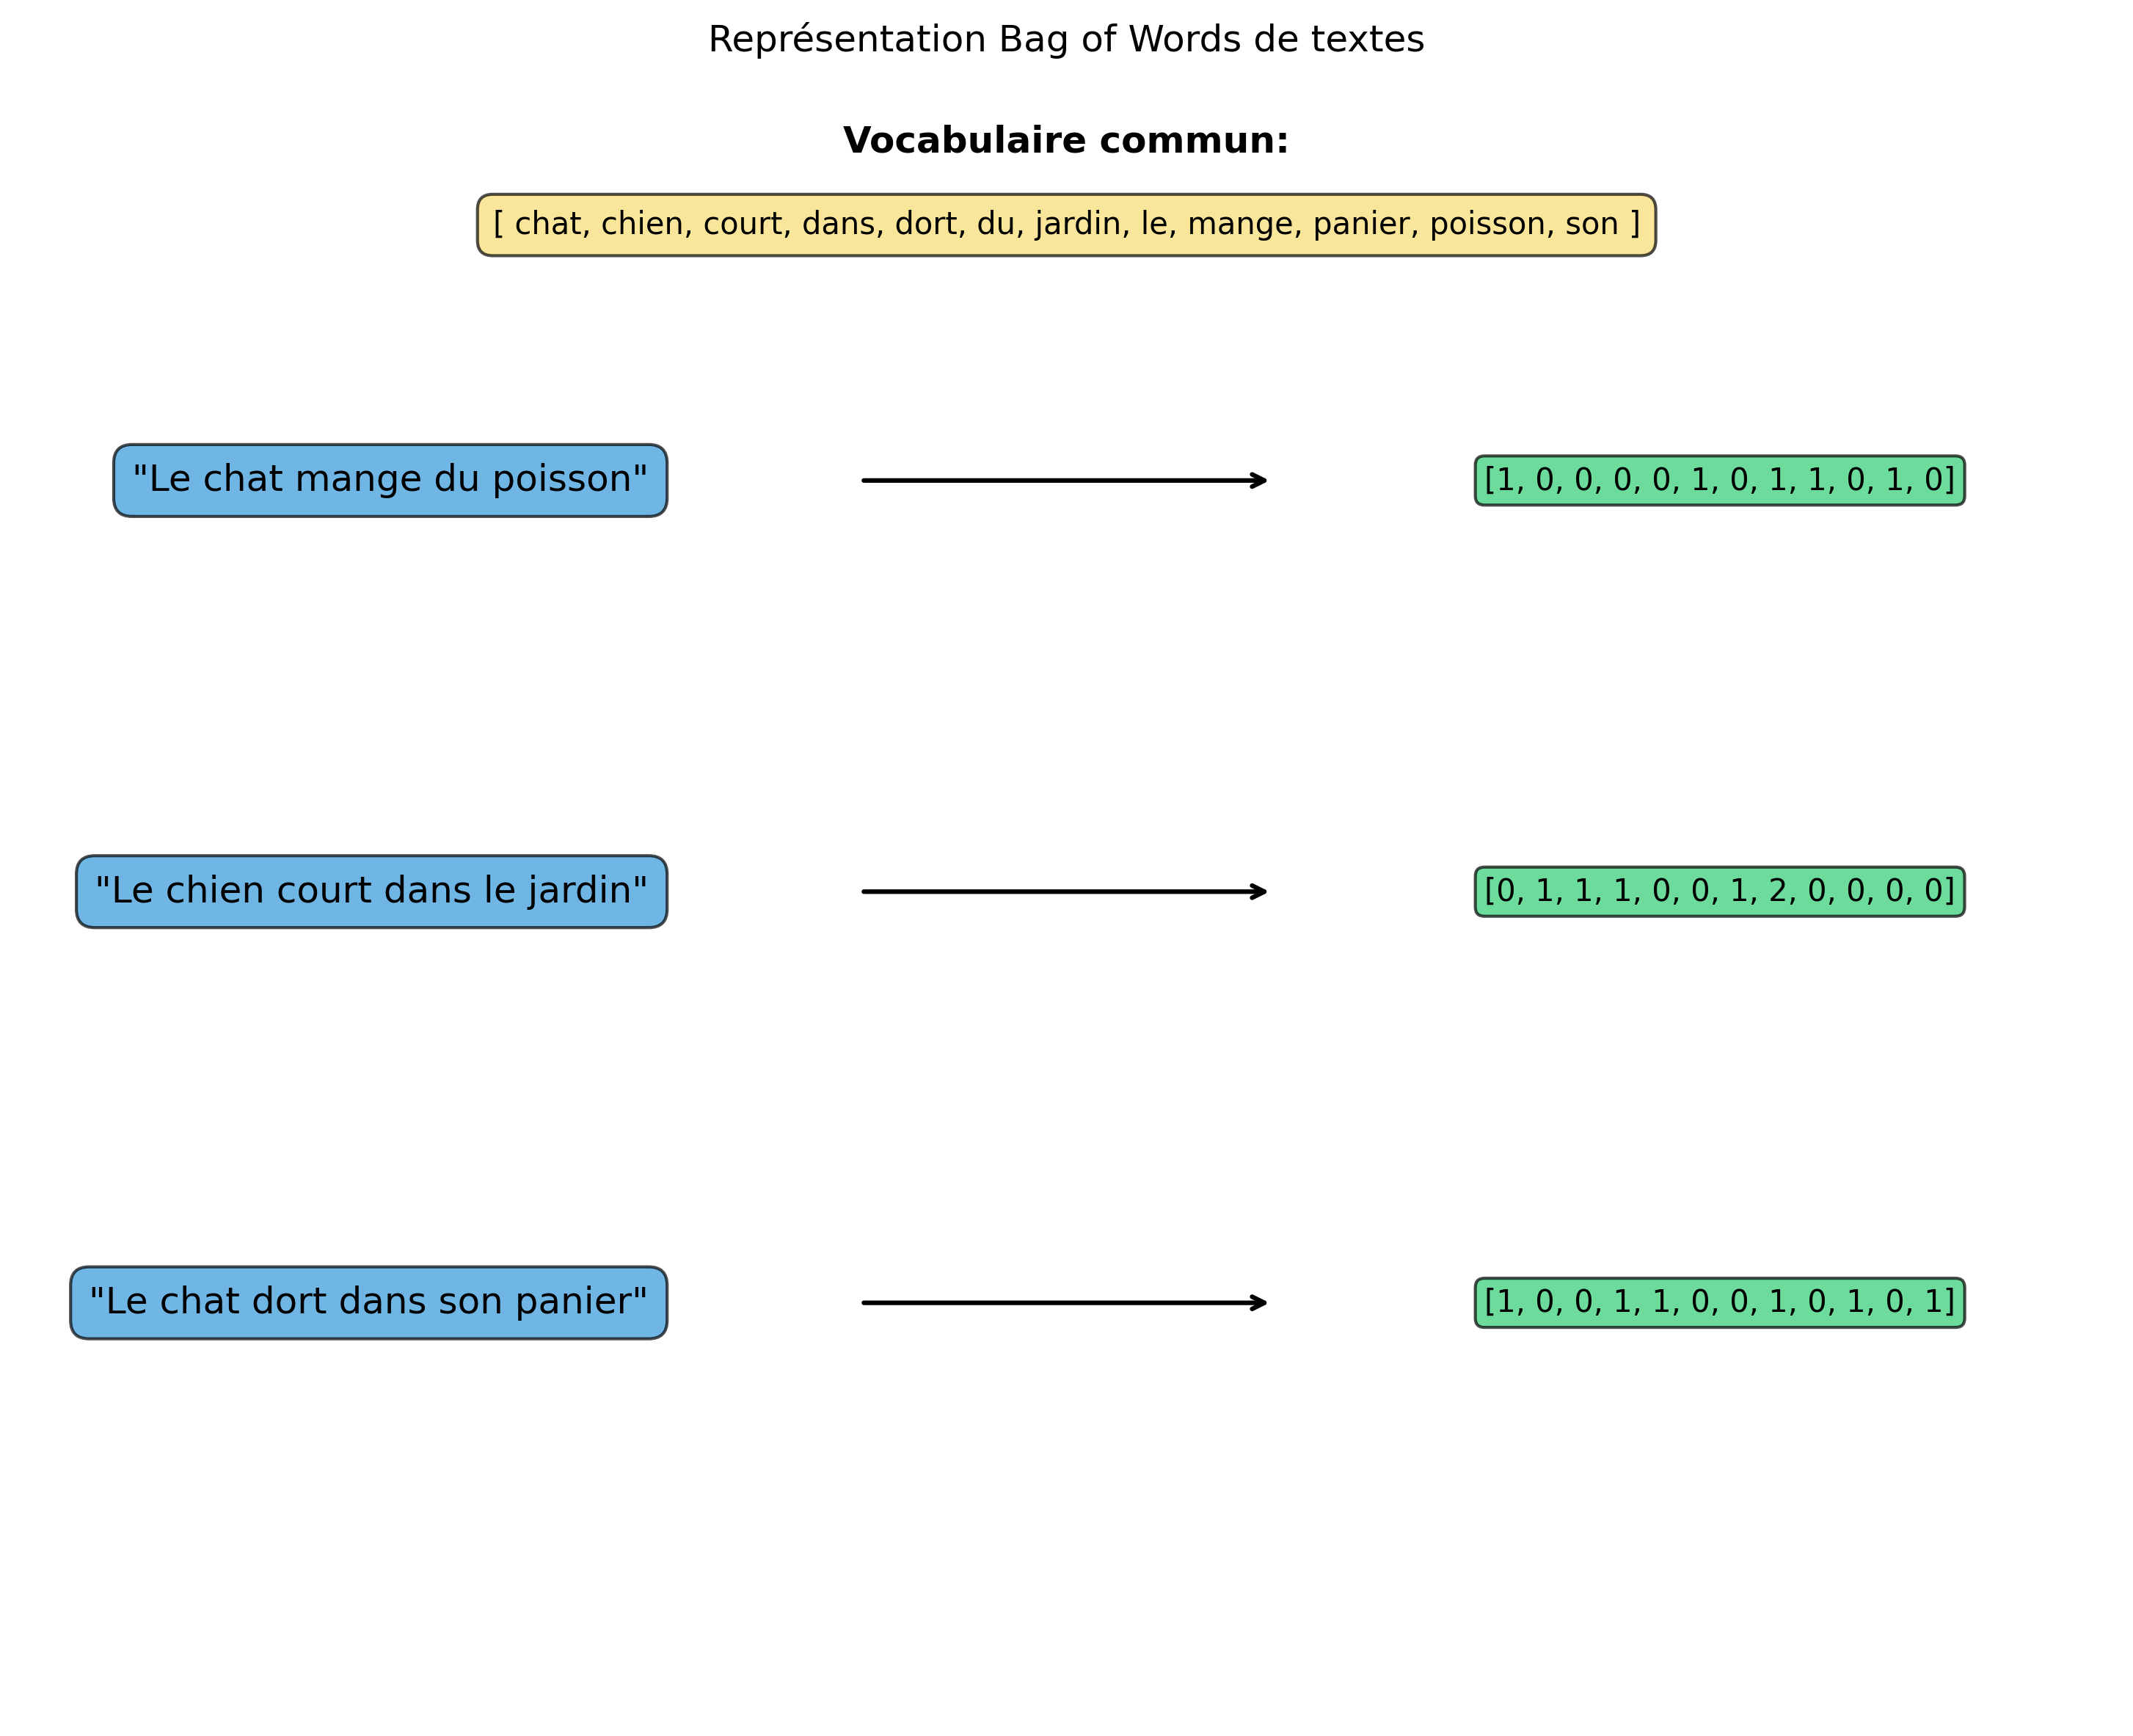
\includegraphics[width=\textwidth]{images/generated/bag_of_words.png}
            \vspace{-0.3cm}
            \begin{center}
                \small{Représentation vectorielle de 3 phrases avec BoW}
            \end{center}
        \end{column}
    \end{columns}
\end{frame}

% Slide: Limites du Bag of Words et introduction au TF-IDF
\begin{frame}{Limites du Bag of Words et Introduction au TF-IDF}
    \begin{columns}
        \begin{column}{0.5\textwidth}
            \textbf{Limites du Bag of Words}
            \begin{itemize}
                \item Perte de la structure grammaticale et syntaxique
                \item Tous les mots ont la même importance
                \item Les mots fréquents (le, la, et, de...) dominent la représentation
                \item Ne capture pas les relations sémantiques entre les mots
                \item Problème de dimensionnalité élevée (vocabulaire large)
            \end{itemize}
        \end{column}
        
        \begin{column}{0.5\textwidth}
            \textbf{TF-IDF: Une amélioration importante}
            \begin{itemize}
                \item \textbf{TF} (Term Frequency): fréquence du terme dans le document
                \item \textbf{IDF} (Inverse Document Frequency): rareté du terme dans le corpus
                \item \textbf{Intuition}: les mots importants apparaissent souvent dans un document mais rarement dans les autres
            \end{itemize}
            \vspace{0.2cm}
            \begin{alertblock}{Avantages du TF-IDF}
                \begin{itemize}
                    \item Réduit l'importance des mots trop fréquents
                    \item Met en valeur les mots discriminants
                    \item Plus efficace pour de nombreuses tâches de NLP
                \end{itemize}
            \end{alertblock}
        \end{column}
    \end{columns}
\end{frame}

% Nouvelle slide: Formule mathématique du TF-IDF
\begin{frame}{Formule Mathématique du TF-IDF}
    \begin{center}
        \Large
        \textbf{Term Frequency (TF)}
        \vspace{0.5cm}
        
        $\text{TF}(t, d) = \frac{\text{nombre d'occurrences de } t \text{ dans } d}{\text{nombre total de termes dans } d}$
        
        \vspace{1cm}
        \textbf{Inverse Document Frequency (IDF)}
        \vspace{0.5cm}
        
        $\text{IDF}(t) = \log\frac{\text{nombre total de documents}}{\text{nombre de documents contenant } t}$
        
        \vspace{1cm}
        \textbf{TF-IDF}
        \vspace{0.5cm}
        
        $\text{TF-IDF}(t, d) = \text{TF}(t, d) \times \text{IDF}(t)$
    \end{center}
\end{frame}

% Slide: Exemple de calcul TF-IDF
\begin{frame}{TF-IDF: Calcul et Applications}
    \begin{columns}
        \begin{column}{0.45\textwidth}
            \textbf{Calcul du TF-IDF}
            \begin{itemize}
                \item Soit un corpus de 3 documents:
                \begin{enumerate}
                    \item "Le chat noir dort sur le canapé"
                    \item "Le chien joue avec la balle dans le jardin"
                    \item "Le chat et le chien courent dans le jardin"
                \end{enumerate}
                \item Pour le mot "chat":
                \begin{itemize}
                    \item TF(chat, doc1) = 1/7
                    \item TF(chat, doc2) = 0
                    \item TF(chat, doc3) = 1/8
                    \item IDF(chat) = log(3/2) = 0.41
                \end{itemize}
                \item TF-IDF(chat, doc1) = 1/7 × 0.41 = 0.059
                \item TF-IDF(chat, doc3) = 1/8 × 0.41 = 0.051
            \end{itemize}
        \end{column}
        \begin{column}{0.55\textwidth}
            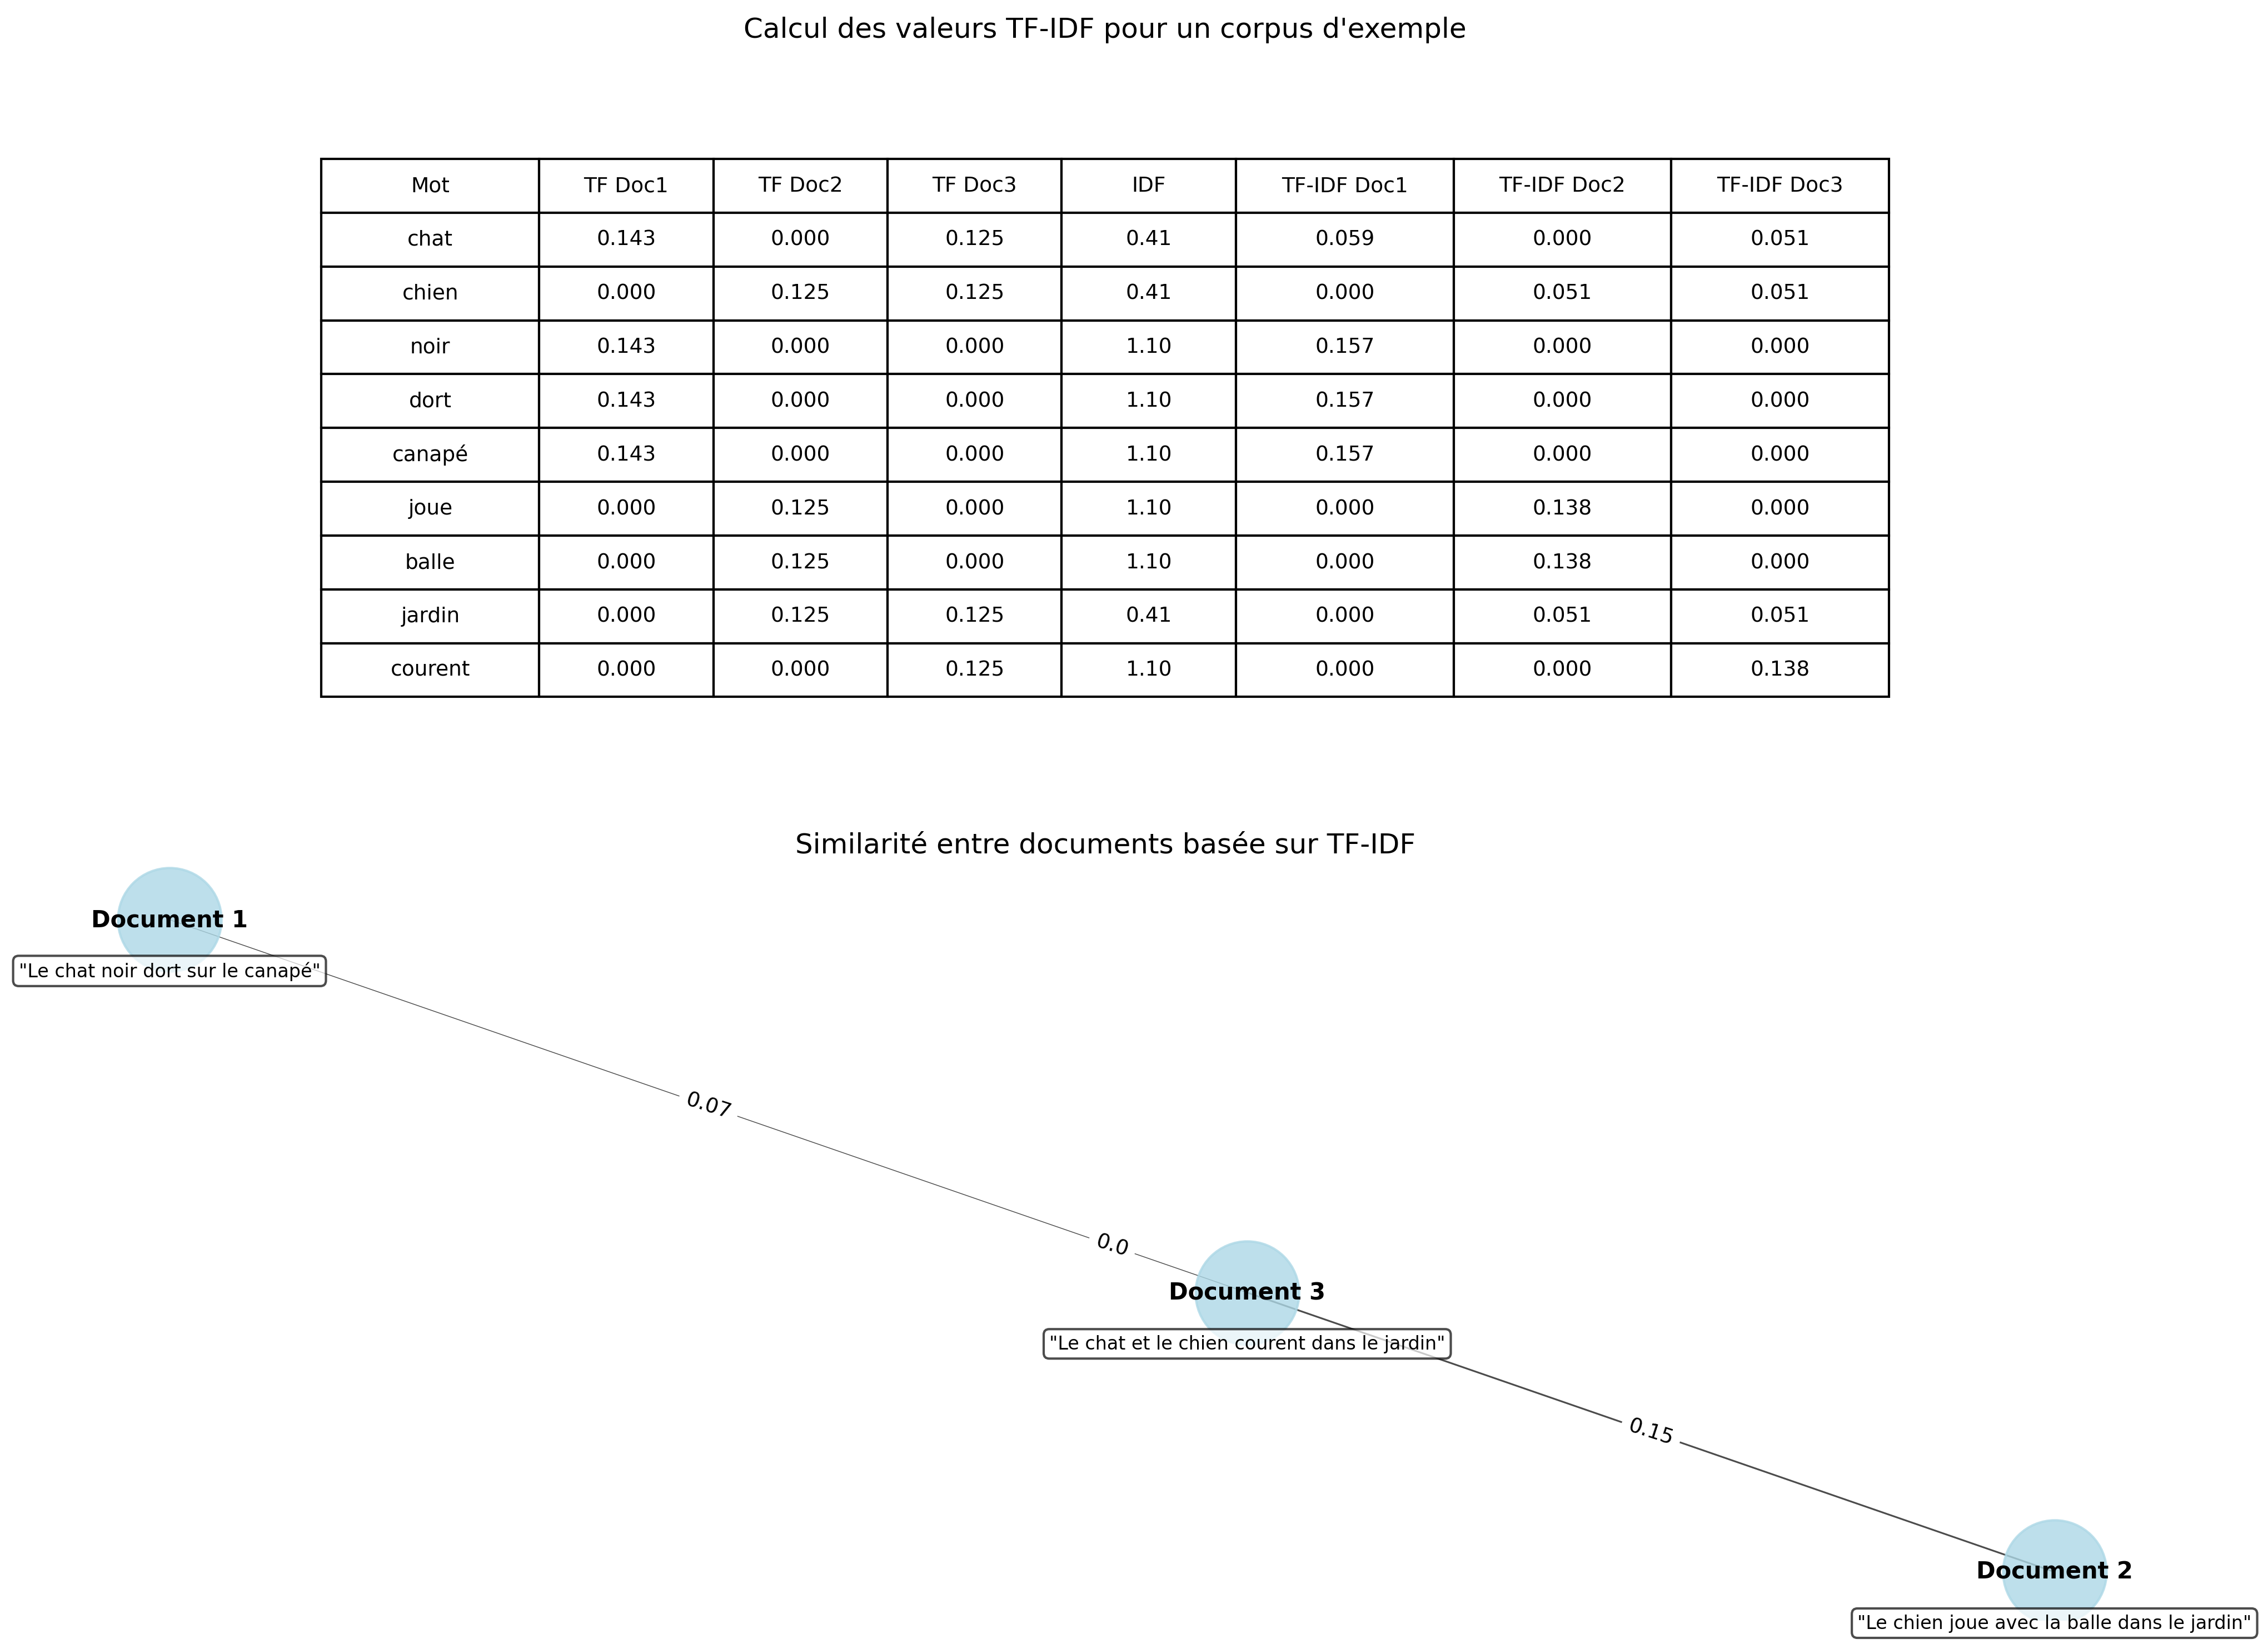
\includegraphics[width=\textwidth]{images/generated/tfidf.png}
            \vspace{-0.3cm}
            \begin{center}
                \small{Calcul et application du TF-IDF à un corpus de documents}
            \end{center}
        \end{column}
    \end{columns}
\end{frame}

% Slide: Classification de sentiment avec TF-IDF et ML classique
\begin{frame}{Classification de Sentiment avec Apprentissage Supervisé}
    \begin{columns}
        \begin{column}{0.55\textwidth}
            \textbf{Pipeline de classification classique}
            \begin{enumerate}
                \item \textbf{Prétraitement} du texte
                \begin{itemize}
                    \item Tokenisation, suppression des stop words
                    \item Normalisation (minuscules, lemmatisation...)
                \end{itemize}
                \item \textbf{Extraction de caractéristiques}
                \begin{itemize}
                    \item Vectorisation (BoW ou TF-IDF)
                    \item Éventuellement, ajout de caractéristiques spécifiques (présence d'émoticons, nombre d'adjectifs...)
                \end{itemize}
                \item \textbf{Entraînement d'un classifieur}
                \begin{itemize}
                    \item Naïve Bayes, Régression Logistique, SVM...
                    \item Évaluation avec validation croisée
                \end{itemize}
                \item \textbf{Prédiction} sur de nouvelles données
            \end{enumerate}
        \end{column}
        \begin{column}{0.45\textwidth}
            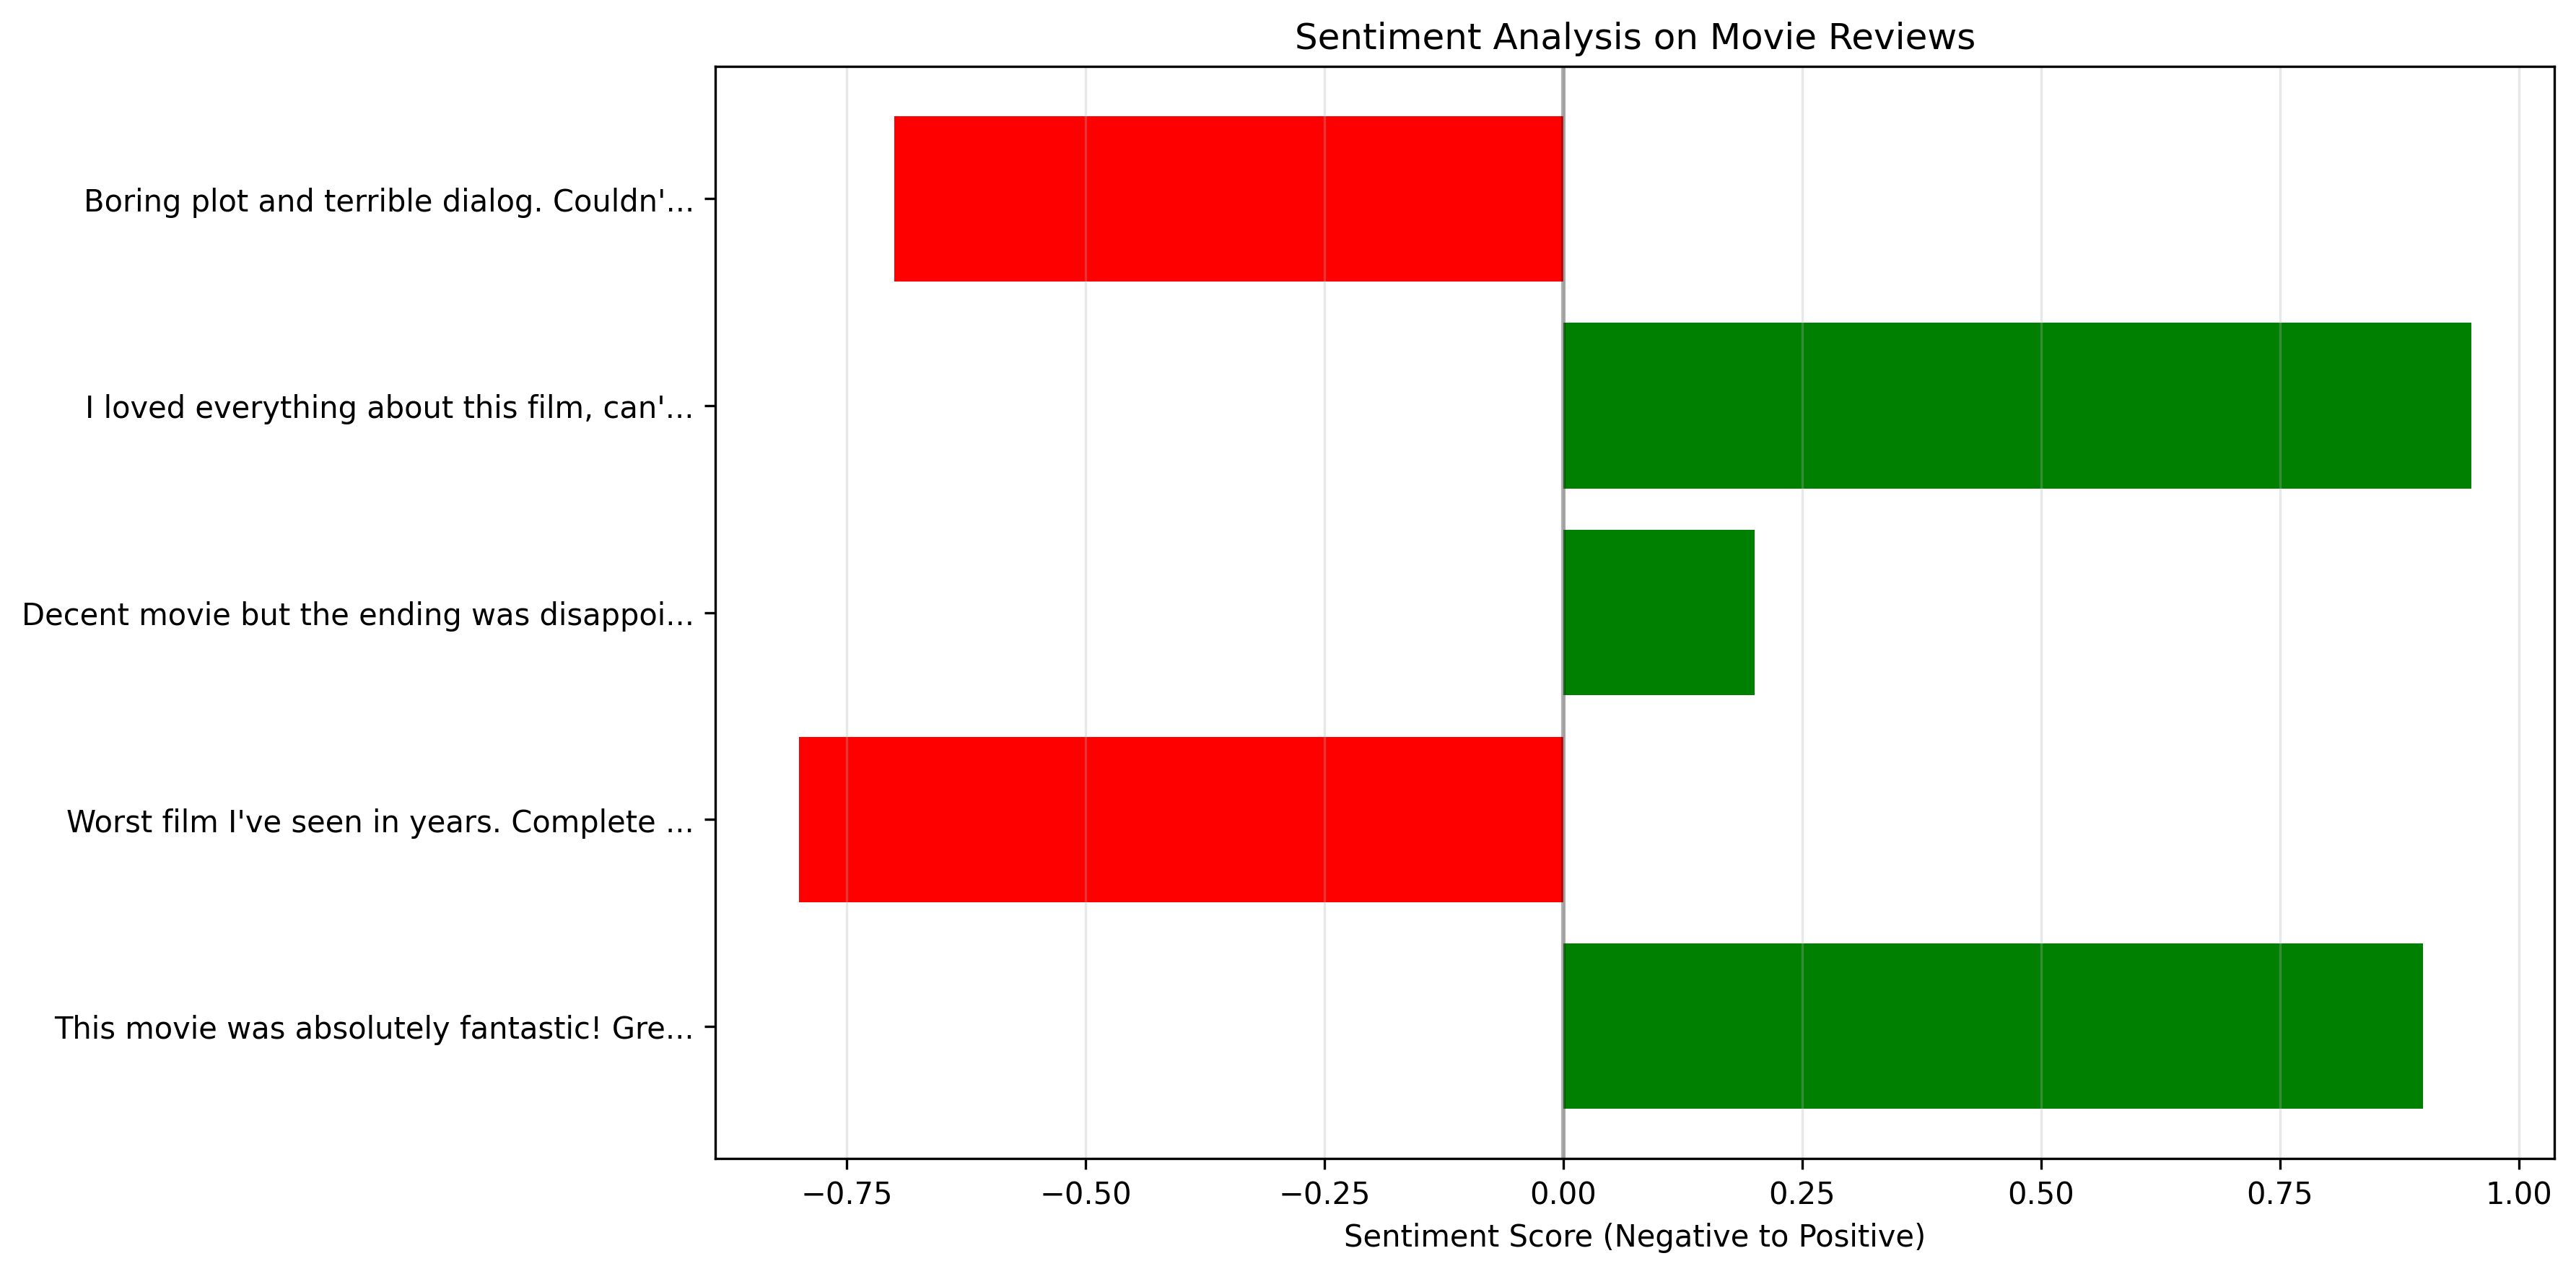
\includegraphics[width=\textwidth]{images/generated/sentiment_analysis.png}
            \begin{center}
                \small{Résultats d'analyse de sentiment sur des critiques}
            \end{center}
            \vspace{0.1cm}
            \begin{alertblock}{Avantages}
                \begin{itemize}
                    \item Modèles légers et interprétables
                    \item Rapides à entraîner et déployer
                    \item Efficaces pour des tâches simples
                \end{itemize}
            \end{alertblock}
        \end{column}
    \end{columns}
\end{frame}

% Nouvelle section: Exemple concret de classification de sentiment
\begin{frame}{Exemple Concret: Classification de Sentiment}
    \begin{exampleblock}{Notre phrase d'exemple}
        \centering
        \large
        "Ce film était vraiment terrible, je ne le recommande à personne!"
    \end{exampleblock}
    
    \vspace{0.3cm}
    \begin{itemize}
        \item Nous allons suivre toutes les étapes pour classifier cette critique de film:
        \begin{enumerate}
            \item \textbf{Prétraitement}: normalisation, lemmatisation, stop words, tokenisation
            \item \textbf{Vectorisation}: représentation en Bag of Words
            \item \textbf{Classification}: entraînement d'un Perceptron Multi-couches
            \item \textbf{Évaluation}: prédiction du sentiment
        \end{enumerate}
        \item Sur un corpus réel, ces étapes seraient appliquées à des milliers d'exemples
    \end{itemize}
\end{frame}

% Slide: Prétraitement de la phrase
\begin{frame}{Prétraitement de la Phrase}
    \begin{columns}
        \begin{column}{0.6\textwidth}
            \begin{enumerate}
                \item \textbf{Normalisation en minuscules}:
                \begin{itemize}
                    \item "ce film était vraiment terrible, je ne le recommande à personne!"
                \end{itemize}
                \vspace{0.2cm}
                \item \textbf{Lemmatisation}:
                \begin{itemize}
                    \item "ce film être vraiment terrible, je ne le recommander à personne!"
                \end{itemize}
                \vspace{0.2cm}
                \item \textbf{Suppression des stop words}:
                \begin{itemize}
                    \item \sout{ce} film \sout{être vraiment} terrible, \sout{je ne le} recommander \sout{à} personne\sout{!}
                    \item → "film terrible recommander personne"
                \end{itemize}
                \vspace{0.2cm}
                \item \textbf{Tokenisation par mot}:
                \begin{itemize}
                    \item $[$"film", "terrible", "recommander", "personne"$]$ → $[4, 9, 8, 7]$
                \end{itemize}
            \end{enumerate}
        \end{column}
        \begin{column}{0.4\textwidth}
            \begin{alertblock}{Stop words en français}
                \small
                \begin{itemize}
                    \item le, la, les, un, une, des
                    \item de, du, à, au, aux
                    \item je, tu, il, elle, nous, vous
                    \item est, sont, être, avoir
                    \item et, ou, mais, donc, car
                    \item très, peu, plus, vraiment
                    \item ...
                \end{itemize}
            \end{alertblock}
        \end{column}
    \end{columns}
\end{frame}

% Slide: Vectorisation avec Bag of Words
\begin{frame}{Vectorisation avec Bag of Words}
    \begin{columns}
        \begin{column}{0.5\textwidth}
            \begin{enumerate}
                \item \textbf{Notre exemple tokenisé}:
                \begin{itemize}
                    \item $[$"film", "terrible", "recommander", "personne"$]$ → $[4, 9, 8, 7]$
                \end{itemize}
                \vspace{0.4cm}
                \item \textbf{Vocabulaire du corpus}:
                \begin{itemize}
                    \item $[$"aimer", "bon", "excellent", "film", "mauvais", "nul", "personne", "recommander", "terrible", "voir", ...] 
                    \item \textit{Indices}: [1, 2, 3, 4, 5, 6, 7, 8, 9, 10, ...]
                \end{itemize}
                \vspace{0.4cm}
                \item \textbf{Vecteur Bag of Words}:
                \begin{itemize}
                    \item $[0, 0, 0, 1, 0, 0, 1, 1, 1, 0, ...]$
                \end{itemize}
            \end{enumerate}
        \end{column}
        \begin{column}{0.5\textwidth}
            \vspace{-0.5cm}
            \begin{center}
                \begin{alertblock}{Note sur les dimensions}
        Dans un cas réel, ce vecteur aurait typiquement \textbf{plusieurs milliers de dimensions}, correspondant à la taille du vocabulaire. Pour notre exemple simplifié, nous travaillons avec un petit vocabulaire.
                \end{alertblock}
            \end{center}
        \end{column}
    \end{columns}
    

\end{frame}

% Slide: Classifieurs pour la classification de sentiment
\begin{frame}{Choix du Classifieur pour la Classification de Sentiment}
    \begin{columns}
        \begin{column}{0.55\textwidth}
            \textbf{Classifieurs traditionnels en NLP}:
            \begin{itemize}
                \item \textbf{Naïve Bayes}
                \begin{itemize}
                    \item Simple, rapide, efficace pour textes courts
                    \item Hypothèse d'indépendance des mots
                \end{itemize}
                \vspace{0.2cm}
                \item \textbf{SVM (Support Vector Machine)}
                \begin{itemize}
                    \item Très performant pour les espaces à haute dimension
                    \item Bonne généralisation, robuste
                \end{itemize}
                \vspace{0.2cm}
                \item \textbf{Régression Logistique}
                \begin{itemize}
                    \item Probabilités interprétables
                    \item Bon équilibre complexité/performance
                \end{itemize}
            \end{itemize}
        \end{column}
        \begin{column}{0.45\textwidth}
            \begin{exampleblock}{Pourquoi un Perceptron?}
                Pour notre exemple, nous utiliserons un \textbf{Perceptron Multi-couches} (MLP):
                \begin{itemize}
                    \item Base des réseaux de neurones modernes
                    \item Introduit les concepts fondamentaux des LLMs
                    \item Permet de comprendre l'apprentissage par gradient
                    \item Évolutif vers des architectures plus complexes
                \end{itemize}
            \end{exampleblock}
        \end{column}
    \end{columns}
\end{frame}

% Slide: Perceptron et MLP - Principes de base
\begin{frame}{Le Perceptron: Unité de Base des Réseaux de Neurones}
    \begin{columns}
        \begin{column}{0.55\textwidth}
            \textbf{Du Perceptron simple au MLP}
            \begin{itemize}
                \item \textbf{Neurone/Perceptron}: unité de calcul élémentaire
                \begin{itemize}
                    \item Prend plusieurs entrées pondérées
                    \item Somme + fonction d'activation
                    \item $y = f(\sum_i w_i x_i + b)$
                \end{itemize}
                \vspace{0.2cm}
                \item \textbf{Rôle dans les réseaux de neurones}:
                \begin{itemize}
                    \item Unité fondamentale de traitement de l'information
                    \item Peut apprendre des frontières linéaires
                \end{itemize}
                \vspace{0.2cm}
                \item \textbf{Limites du perceptron simple}:
                \begin{itemize}
                    \item Ne peut modéliser que des relations linéaires
                    \item Nécessite des fonctions d'activation non-linéaires
                    \item Doit être organisé en réseaux complexes pour des tâches avancées
                \end{itemize}
            \end{itemize}
        \end{column}
        \begin{column}{0.45\textwidth}
            \begin{center}
                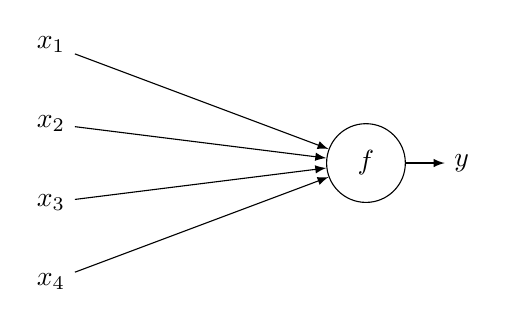
\begin{tikzpicture}[>=latex]
                    % Inputs
                    \foreach \i in {1,...,4}
                    {
                        \node (Input-\i) at (0,-\i) {$x_\i$};
                    }

                    % Single Neuron
                    \node[draw, circle, minimum size=1cm] (Neuron) at (4,-2.5) {$f$};
                    % Output for the neuron
                    \draw[->] (Neuron) -- ++(1,0) node[right] {$y$};

                    % Draw connections from inputs to the neuron
                    \foreach \i in {1,...,4}
                    {
                        \draw[->] (Input-\i) -- (Neuron);
                    }
                \end{tikzpicture}
            \end{center}
            \vspace{0.1cm}
            \begin{alertblock}{Perceptron vs Neurone Biologique}
                Bien que simplifié, le perceptron s'inspire du neurone biologique: il reçoit des entrées (comme les dendrites), les pondère (comme les synapses), les agrège et produit une sortie (comme l'axone).
            \end{alertblock}
        \end{column}
    \end{columns}
\end{frame}

% Nouvelle slide: Fonctions d'activation
\begin{frame}{Fonctions d'Activation: Introduire la Non-Linéarité}
    \begin{columns}
        \begin{column}{0.55\textwidth}
            \textbf{Pourquoi des fonctions d'activation?}
            \begin{itemize}
                \item \textbf{Fonctions d'activation}: introduisent la non-linéarité
                \begin{itemize}
                    \item Transforment la somme pondérée en sortie
                    \item Permettent d'apprendre des motifs complexes
                \end{itemize}
                \vspace{0.2cm}
                \item \textbf{Types de fonctions d'activation}:
                \begin{itemize}
                    \item Sigmoïde: $\sigma(x) = \frac{1}{1+e^{-x}}$ (de 0 à 1)
                    \item Tanh: $\tanh(x) = \frac{e^x - e^{-x}}{e^x + e^{-x}}$ (de -1 à 1)
                \end{itemize}
                \vspace{0.2cm}
                \item \textbf{ReLU} (Rectified Linear Unit):
                \begin{itemize}
                    \item $f(x) = \max(0, x)$ - Simple mais efficace
                    \item Utilisée dans la majorité des réseaux modernes
                \end{itemize}
            \end{itemize}
        \end{column}
        \begin{column}{0.45\textwidth}
            \begin{center}
                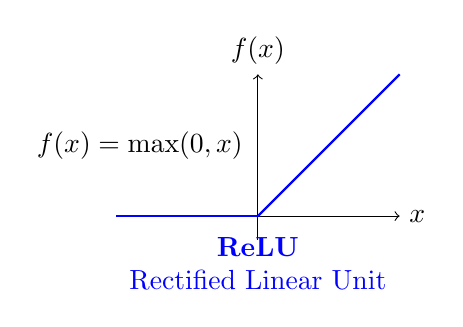
\begin{tikzpicture}[scale=0.6]
                    % Axes
                    \draw[->] (-3,0) -- (3,0) node[right] {$x$};
                    \draw[->] (0,-0.5) -- (0,3) node[above] {$f(x)$};
                    
                    % ReLU function
                    \draw[thick, blue] (-3,0) -- (0,0);
                    \draw[thick, blue] (0,0) -- (3,3);
                    
                    % Labels
                    \node at (-2.5,1.5) {$f(x) = \max(0,x)$};
                    \node[blue, align=center] at (0,-1) {\textbf{ReLU}\\ Rectified Linear Unit};
                \end{tikzpicture}
            \end{center}
            \begin{alertblock}{Pourquoi la non-linéarité?}
                Sans fonctions d'activation non-linéaires, un réseau à plusieurs couches serait équivalent à un simple modèle linéaire, incapable d'apprendre des motifs complexes.
            \end{alertblock}
        \end{column}
    \end{columns}
\end{frame}

% Nouvelle slide: Couches de neurones et MLP
\begin{frame}{Architecture des Réseaux de Neurones}
    \begin{columns}
        \begin{column}{0.55\textwidth}
            \textbf{Organisation en couches}
            \begin{itemize}
                \item \textbf{Couche de neurones}: ensemble de neurones en parallèle
                \begin{itemize}
                    \item Couche d'entrée: données brutes
                    \item Couche(s) cachée(s): représentations intermédiaires
                    \item Couche de sortie: prédictions
                \end{itemize}
                \vspace{0.2cm}
                \item \textbf{MLP (Multi-Layer Perceptron)}: réseau à plusieurs couches
                \begin{itemize}
                    \item Capable d'apprendre des frontières non linéaires
                    \item Pour sentiment: 2 neurones de sortie (positif/négatif)
                \end{itemize}
            \end{itemize}
        \end{column}
        \begin{column}{0.45\textwidth}
            \begin{center}
                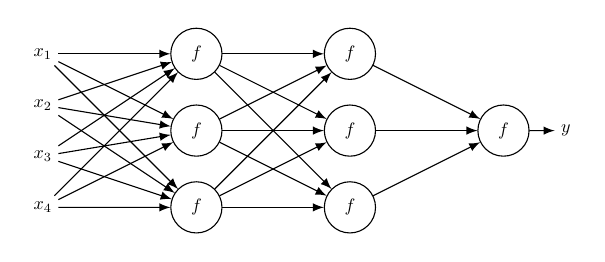
\begin{tikzpicture}[>=latex, node distance=1.5cm, scale=0.65, transform shape]
                    % Inputs
                    \foreach \i in {1,...,4}
                    {
                        \node (Input-\i) at (0,-\i) {$x_\i$};
                    }

                    % First Hidden Layer
                    \foreach \i in {1,...,3}
                    {
                        \node[draw, circle, minimum size=1cm] (Hidden1-\i) at (3,{-\i*1.5+0.5}) {$f$};
                    }

                    % Second Hidden Layer
                    \foreach \i in {1,...,3}
                    {
                        \node[draw, circle, minimum size=1cm] (Hidden2-\i) at (6,{-\i*1.5+0.5}) {$f$};
                    }

                    % Output Layer
                    \node[draw, circle, minimum size=1cm] (Output) at (9,-2.5) {$f$};

                    % Draw connections from inputs to the first hidden layer
                    \foreach \i in {1,...,4}
                    {
                        \foreach \j in {1,...,3}
                        {
                            \draw[->] (Input-\i) -- (Hidden1-\j);
                        }
                    }

                    % Draw connections between first and second hidden layer
                    \foreach \i in {1,...,3}
                    {
                        \foreach \j in {1,...,3}
                        {
                            \draw[->] (Hidden1-\i) -- (Hidden2-\j);
                        }
                    }

                    % Draw connections from the second hidden layer to the output
                    \foreach \i in {1,...,3}
                    {
                        \draw[->] (Hidden2-\i) -- (Output);
                    }

                    % Output
                    \draw[->] (Output) -- ++(1,0) node[right] {$y$};
                \end{tikzpicture}
            \end{center}
            \vspace{0.2cm}
            \begin{center}
                \small{Architecture d'un MLP avec deux couches cachées}
            \end{center}
        \end{column}
    \end{columns}
\end{frame}

% Slide: Apprentissage d'un réseau de neurones
\begin{frame}{Apprentissage d'un Réseau de Neurones}
    \begin{columns}
        \begin{column}{0.6\textwidth}
            \textbf{Principes clés de l'apprentissage}
            \begin{enumerate}
                \item \textbf{Phase de propagation avant (forward)}:
                \begin{itemize}
                    \item Les entrées traversent le réseau de gauche à droite
                    \item Chaque couche applique sa transformation
                    \item On obtient une prédiction en sortie
                \end{itemize}
                \item \textbf{Calcul de l'erreur}:
                \begin{itemize}
                    \item Comparaison entre prédiction et vérité terrain
                    \item Utilisation d'une fonction de perte (loss)
                \end{itemize}
                \item \textbf{Rétropropagation (backpropagation)}:
                \begin{itemize}
                    \item Calcul des gradients de l'erreur
                    \item Propagation des gradients de droite à gauche
                \end{itemize}
                \item \textbf{Mise à jour des poids}:
                \begin{itemize}
                    \item Utilisation de la descente de gradient
                    \item $w_{new} = w_{old} - \alpha \cdot \nabla_w L$
                \end{itemize}
            \end{enumerate}
        \end{column}
        \begin{column}{0.4\textwidth}
            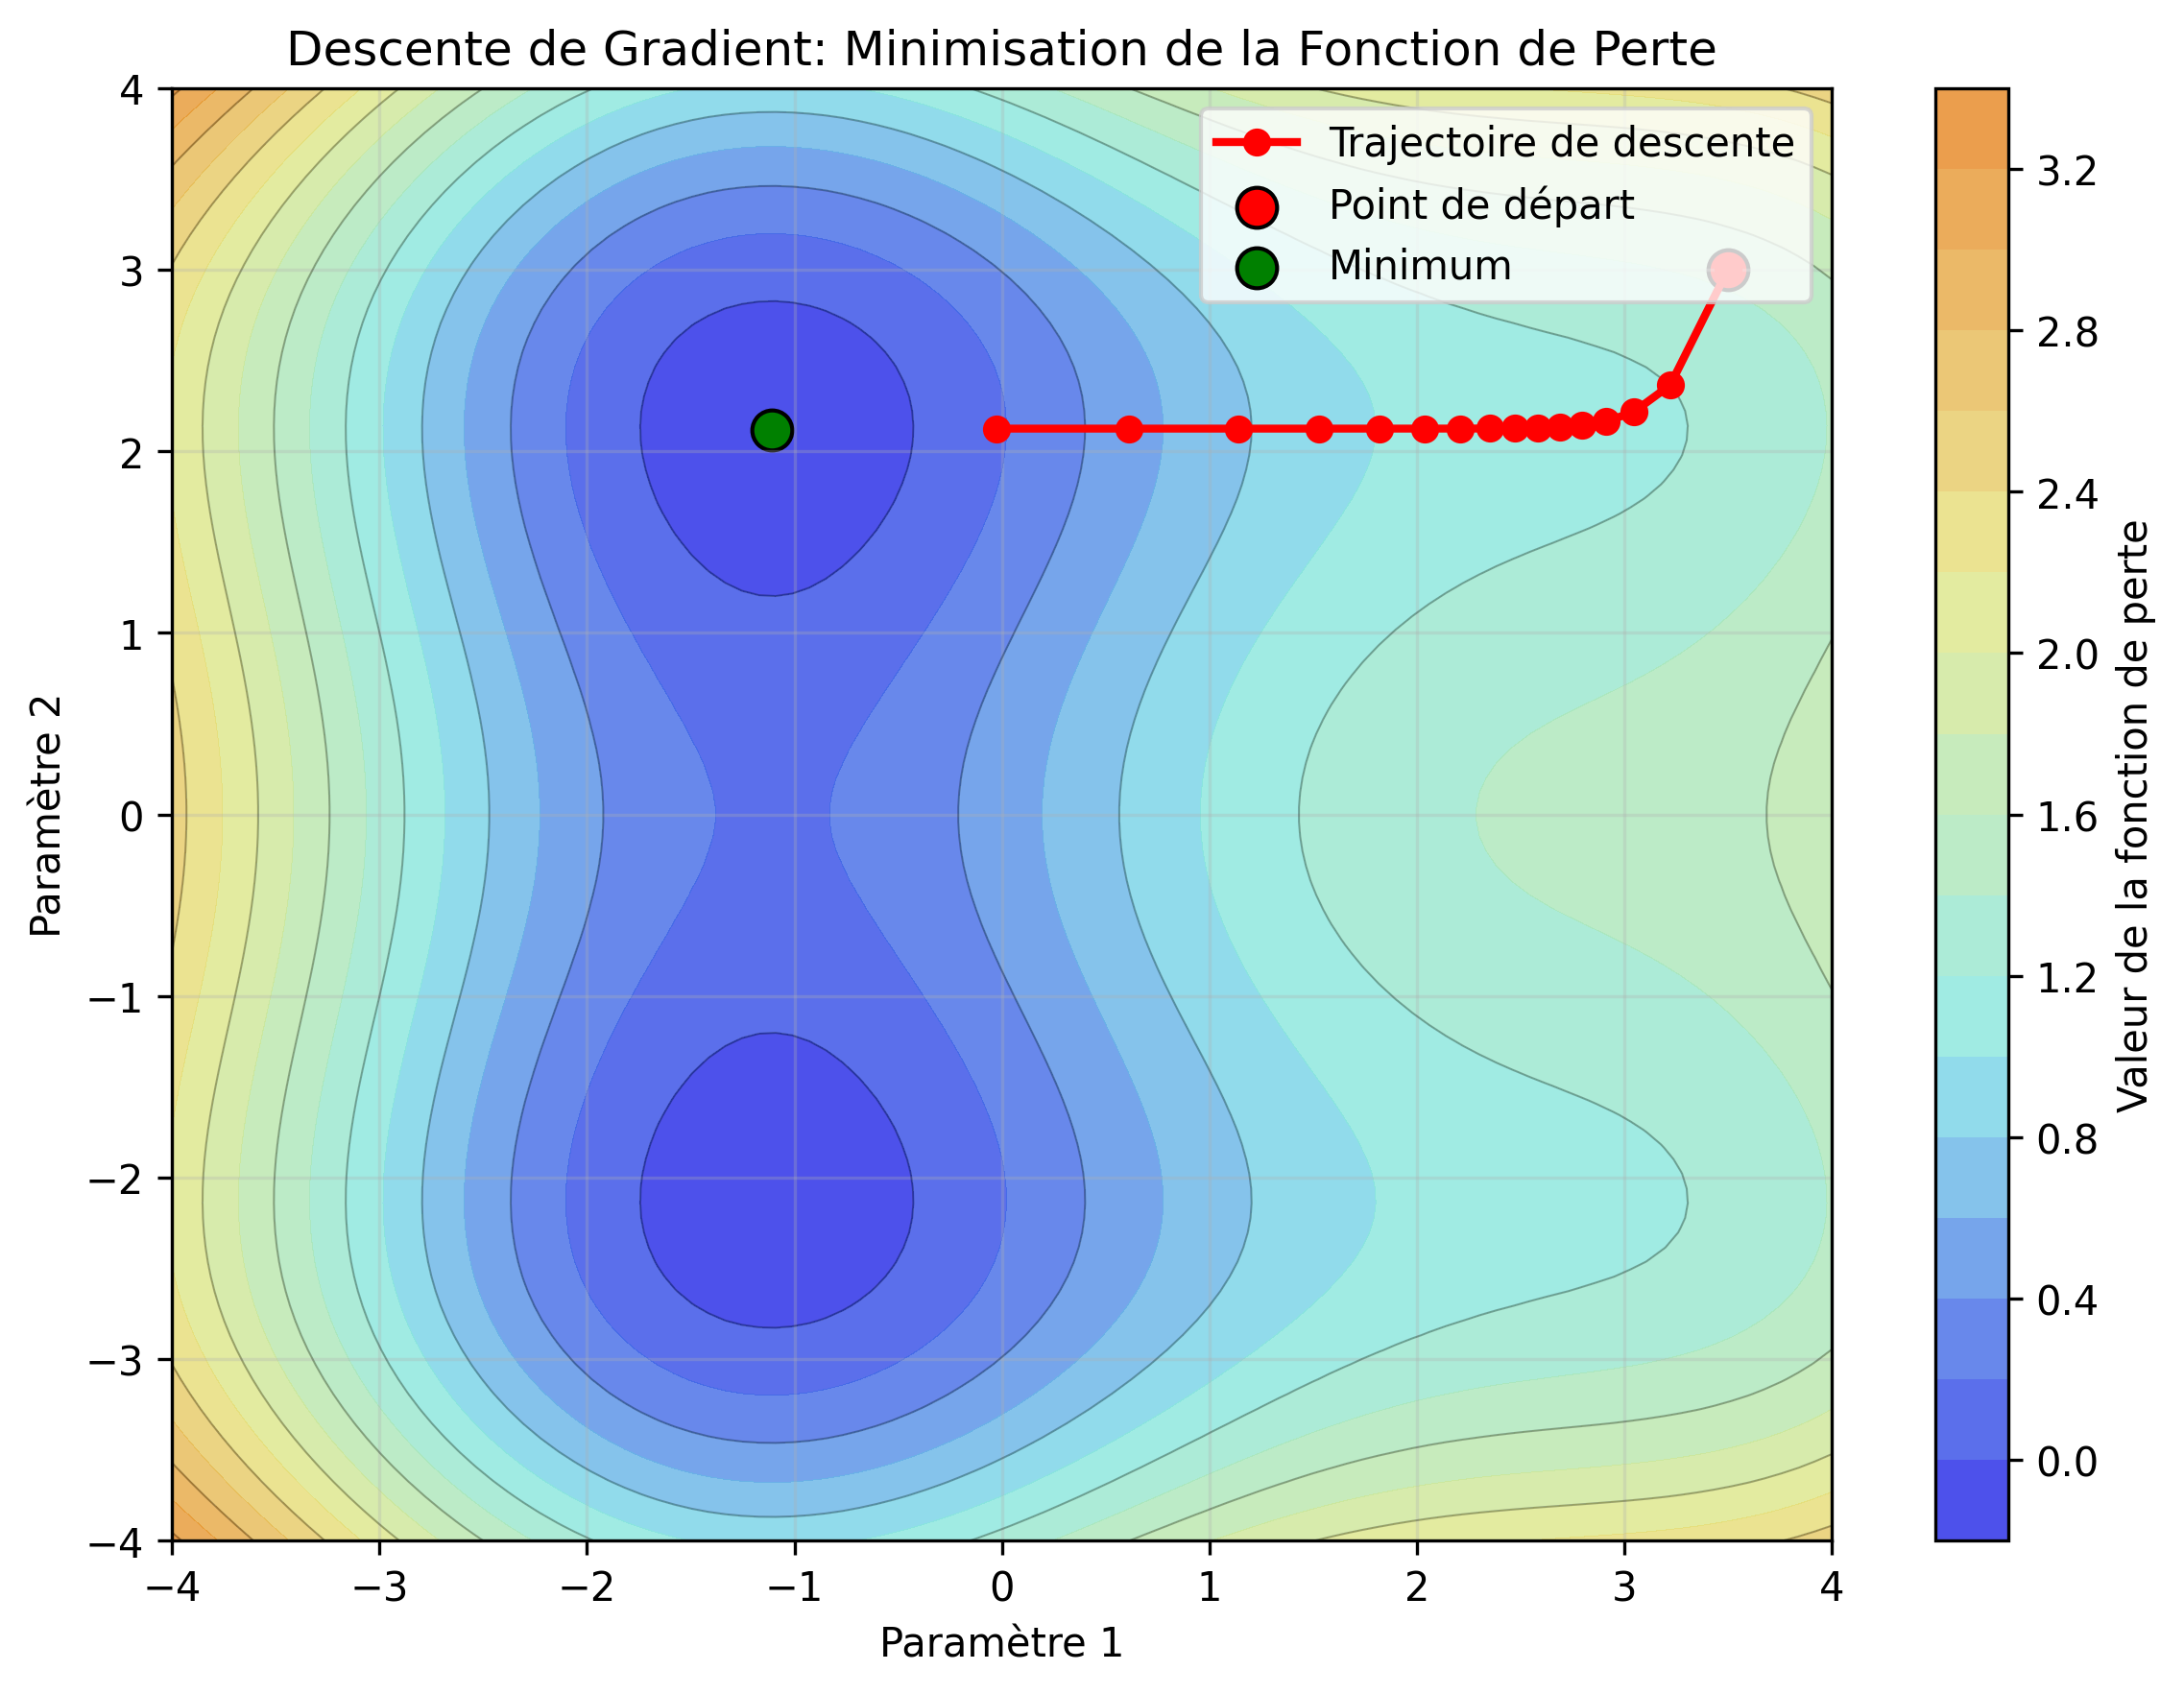
\includegraphics[width=\textwidth]{images/gradient_descent.png}
            \vspace{-0.3cm}
            \begin{center}
                \small{Descente de gradient: minimisation de la fonction de perte}
            \end{center}
        \end{column}
    \end{columns}
\end{frame}

% Slide: Fonctions de perte pour la classification
\begin{frame}{Fonctions de Perte pour la Classification}
    \begin{columns}
        \begin{column}{0.55\textwidth}
            \textbf{Entropie croisée (Cross-Entropy)}
            \begin{itemize}
                \item \textbf{Définition mathématique}:
                \begin{equation}
                L = -\sum_{i=1}^{C} y_i \log(\hat{y}_i)
                \end{equation}
                où $y_i$ est la vérité terrain, $\hat{y}_i$ la prédiction pour la classe $i$
                \vspace{0.3cm}
                \item \textbf{Propriétés}:
                \begin{itemize}
                    \item Pénalise fortement les mauvaises prédictions confiantes
                    \item Récompense les bonnes prédictions confiantes
                    \item Idéale pour la classification multi-classes
                \end{itemize}
            \end{itemize}
        \end{column}
        \begin{column}{0.45\textwidth}
            \begin{exampleblock}{Exemple pour notre cas}
                Pour notre critique de film négative:
                \begin{itemize}
                    \item Vérité terrain: [0, 1] (négatif)
                    \item Mauvaise prédiction: [0.9, 0.1]
                    \item Perte: $-(0 \times \log(0.9) + 1 \times \log(0.1)) \approx 2.3$
                    \vspace{0.3cm}
                    \item Bonne prédiction: [0.1, 0.9]
                    \item Perte: $-(0 \times \log(0.1) + 1 \times \log(0.9)) \approx 0.1$
                \end{itemize}
            \end{exampleblock}
        \end{column}
    \end{columns}
\end{frame}

% Nouvelle slide: Calcul du gradient par rétropropagation
\begin{frame}{Calcul du Gradient par Rétropropagation}
    \begin{columns}
        \begin{column}{0.5\textwidth}
            \textbf{Principe de la rétropropagation}
            \begin{itemize}
                \item \textbf{Objectif}: calculer $\frac{\partial L}{\partial w_{ij}^{(l)}}$ pour chaque poids
                \item \textbf{Solution}: appliquer la règle de dérivation en chaîne
            \end{itemize}
            
            \vspace{0.3cm}
            \textbf{Mécanisme de la rétropropagation}
            \begin{itemize}
                \item \textbf{Étape 1}: Calculer l'erreur à la couche de sortie
                \begin{itemize}
                    \item $\delta^{(L)} = \frac{\partial L}{\partial y_{pred}} \cdot f'(z^{(L)})$
                \end{itemize}
                \item \textbf{Étape 2}: Propager l'erreur vers les couches inférieures
                \begin{itemize}
                    \item $\delta^{(l)} = (W^{(l+1)})^T \delta^{(l+1)} \cdot f'(z^{(l)})$
                \end{itemize}
                \item \textbf{Étape 3}: Calculer les gradients pour chaque poids
                \begin{itemize}
                    \item $\frac{\partial L}{\partial W^{(l)}} = a^{(l-1)} \cdot (\delta^{(l)})^T$
                \end{itemize}
            \end{itemize}
        \end{column}
        \begin{column}{0.5\textwidth}
            \begin{center}
                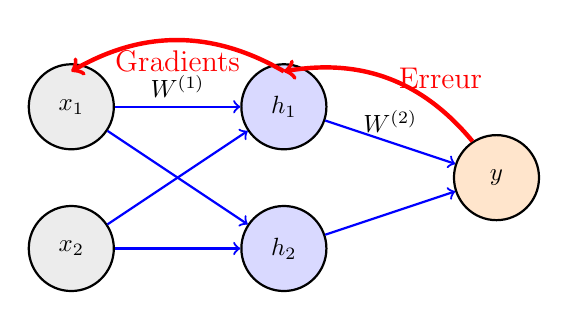
\begin{tikzpicture}[scale=0.9, transform shape]
                    % Simplified network with larger elements
                    % Input layer
                    \node[circle, draw, thick, minimum size=1.2cm, fill=lightgray!30] (x1) at (0,0) {$x_1$};
                    \node[circle, draw, thick, minimum size=1.2cm, fill=lightgray!30] (x2) at (0,-2) {$x_2$};
                    
                    % Hidden layer
                    \node[circle, draw, thick, minimum size=1.2cm, fill=blue!15] (h1) at (3,0) {$h_1$};
                    \node[circle, draw, thick, minimum size=1.2cm, fill=blue!15] (h2) at (3,-2) {$h_2$};
                    
                    % Output layer
                    \node[circle, draw, thick, minimum size=1.2cm, fill=orange!20] (y) at (6,-1) {$y$};
                    
                    % Forward connections
                    \draw[->, thick, blue] (x1) -- (h1) node[midway, above, black] {$W^{(1)}$};
                    \draw[->, thick, blue] (x1) -- (h2);
                    \draw[->, thick, blue] (x2) -- (h1);
                    \draw[->, thick, blue] (x2) -- (h2);
                    \draw[->, thick, blue] (h1) -- (y) node[midway, above, black] {$W^{(2)}$};
                    \draw[->, thick, blue] (h2) -- (y);
                    
                    % Backpropagation arrows - made more visible
                    \draw[->, ultra thick, red] (y) to[bend right=30] node[midway, right, font=\large, red] {Erreur} (3,0.5);
                    \draw[->, ultra thick, red] (3,0.5) to[bend right=30] node[midway, below, font=\large, red] {Gradients} (0,0.5);
                \end{tikzpicture}
            \end{center}
            
            \begin{alertblock}{Efficacité de la rétropropagation}
                La rétropropagation permet de calculer tous les gradients en une seule passe arrière, réduisant significativement la complexité de calcul.
            \end{alertblock}
        \end{column}
    \end{columns}
\end{frame}

% Nouvelle slide: Mise à jour des poids
\begin{frame}{Mise à Jour des Poids: Optimisation par Descente de Gradient}
    \begin{columns}
        \begin{column}{0.5\textwidth}
            \textbf{Algorithme de descente de gradient}
            \begin{itemize}
                \item \textbf{Principe}: mise à jour itérative des paramètres
                \item \textbf{Formule générale}:
                \begin{equation}
                W^{(l)} \leftarrow W^{(l)} - \eta \cdot \frac{\partial L}{\partial W^{(l)}}
                \end{equation}
                où $\eta$ est le taux d'apprentissage
                
                \vspace{0.2cm}
                \item \textbf{Variantes de l'algorithme}:
                \begin{itemize}
                    \item \textbf{Batch}: calcul sur l'ensemble du dataset
                    \item \textbf{Mini-batch}: calcul sur un sous-ensemble
                    \item \textbf{Stochastique (SGD)}: calcul sur un exemple à la fois
                \end{itemize}
            \end{itemize}
            
            \vspace{0.3cm}
            \textbf{Optimiseurs avancés}
            \begin{itemize}
                \item \textbf{Adam}: adapte le taux d'apprentissage par paramètre
                \item \textbf{RMSprop}: utilise moyenne mobile des gradients
                \item \textbf{Momentum}: ajoute de l'inertie à la descente
            \end{itemize}
        \end{column}
        
        \begin{column}{0.5\textwidth}
            
            \begin{alertblock}{Importance du taux d'apprentissage}
                \begin{itemize}
                    \item \textbf{Trop petit}: convergence très lente
                    \item \textbf{Trop grand}: oscillations ou divergence
                    \item \textbf{Idéal}: adaptatif selon la forme de la fonction de perte
                \end{itemize}
            \end{alertblock}
        \end{column}
    \end{columns}
\end{frame}

% Slide: Résumé du processus complet de classification
\begin{frame}{Résumé du Processus Complet de Classification}
    \begin{enumerate}
        \item \textbf{Préparation des données}
        \begin{itemize}
            \item Prétraitement: normalisation, lemmatisation, stop words
            \item Tokenisation: découpage en unités lexicales (mots)
            \item Vectorisation: transformation en représentation numérique (BoW)
        \end{itemize}
        \vspace{0.1cm}
        \item \textbf{Conception du modèle}
        \begin{itemize}
            \item Architecture MLP: couche d'entrée (taille du vocabulaire), couche(s) cachée(s), couche de sortie (2 neurones)
            \item Choix des hyperparamètres: nombre de couches, nombre de neurones, fonction d'activation
        \end{itemize}
        \vspace{0.1cm}
        \item \textbf{Entraînement}
        \begin{itemize}
            \item Propagation avant: calcul des prédictions
            \item Calcul de la perte: entropie croisée
            \item Rétropropagation: calcul des gradients
            \item Optimisation: mise à jour des poids par descente de gradient
        \end{itemize}
        \vspace{0.1cm}
        \item \textbf{Évaluation et prédiction}
        \begin{itemize}
            \item Métriques: précision, rappel, F1-score
            \item Application à de nouvelles données
        \end{itemize}
    \end{enumerate}
\end{frame}

% Nouvelle section sur la génération de texte
\section{Génération de Texte avec Modèles N-gram}
% Slide: Titre de la section sur la génération de texte
\begin{frame}
    \begin{center}
        \Huge{\textbf{Génération de Texte}}
        \vspace{0.5cm}
        
        \Large{Modèles N-gram et approches statistiques}
        \vspace{1cm}
    \end{center}
\end{frame}

% Slide: Introduction à la génération de texte
\begin{frame}{Introduction à la Génération de Texte}
    \begin{columns}
        \begin{column}{0.55\textwidth}
            \begin{itemize}
                \item La \textbf{génération de texte} est une tâche fondamentale du NLP
                \item Elle vise à produire du texte nouveau et cohérent
                \item Applications:
                \begin{itemize}
                    \item Complétion automatique de phrases
                    \item Génération de résumés
                    \item Création de contenu (articles, poésie)
                    \item Chatbots et assistants conversationnels
                \end{itemize}
                \vspace{0.3cm}
                \item Approches principales:
                \begin{itemize}
                    \item \textbf{Modèles statistiques}: N-grams
                    \item \textbf{Réseaux de neurones}: RNN, LSTM, Transformers
                    \item \textbf{Modèles hybrides}: combinaison des approches
                \end{itemize}
            \end{itemize}
        \end{column}
        \begin{column}{0.45\textwidth}
            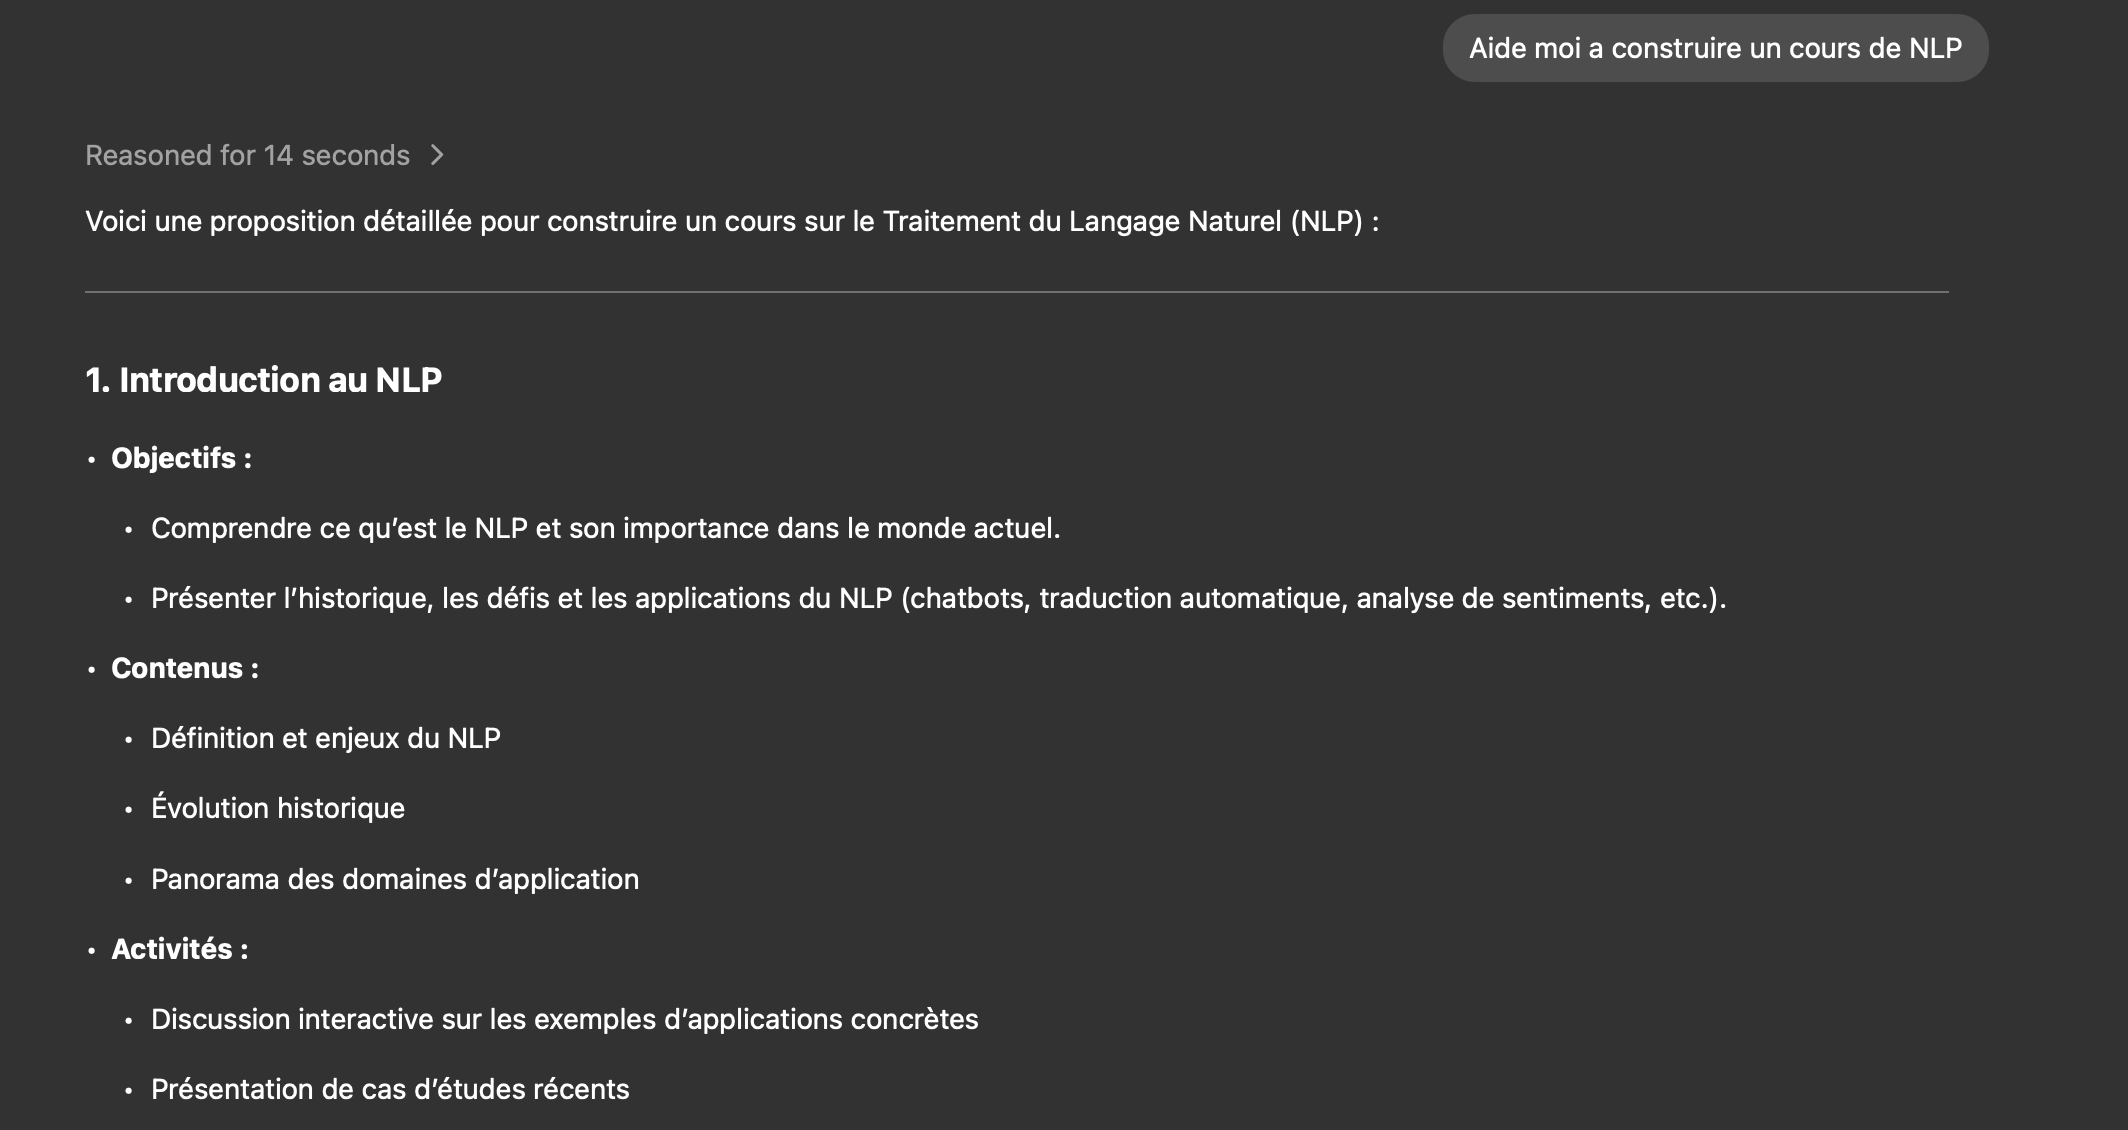
\includegraphics[width=\textwidth]{images/chatbot.png}
            \begin{center}
                \small{Exemple de génération de texte dans un assistant conversationnel}
            \end{center}
        \end{column}
    \end{columns}
\end{frame}

% Slide: Qu'est-ce qu'un modèle N-gram?
\begin{frame}{Qu'est-ce qu'un Modèle N-gram?}
    \begin{columns}
        \begin{column}{0.55\textwidth}
            \textbf{Principe des modèles N-gram}
            \begin{itemize}
                \item Modèle \textbf{statistique} basé sur les probabilités de séquences
                \item Un n-gram est une \textbf{séquence de n éléments} consécutifs
                \begin{itemize}
                    \item \textbf{Unigramme (n=1)}: mots individuels 
                    \item \textbf{Bigramme (n=2)}: paires de mots consécutifs
                    \item \textbf{Trigramme (n=3)}: triplets de mots consécutifs
                \end{itemize}
                \vspace{0.3cm}
                \item \textbf{Hypothèse markovienne}: la probabilité d'un mot dépend uniquement des n-1 mots précédents
                \begin{itemize}
                    \item Simplification qui rend le calcul possible
                    \item Limitation: ne capture pas les dépendances à long terme
                \end{itemize}
            \end{itemize}
        \end{column}
        \begin{column}{0.45\textwidth}
            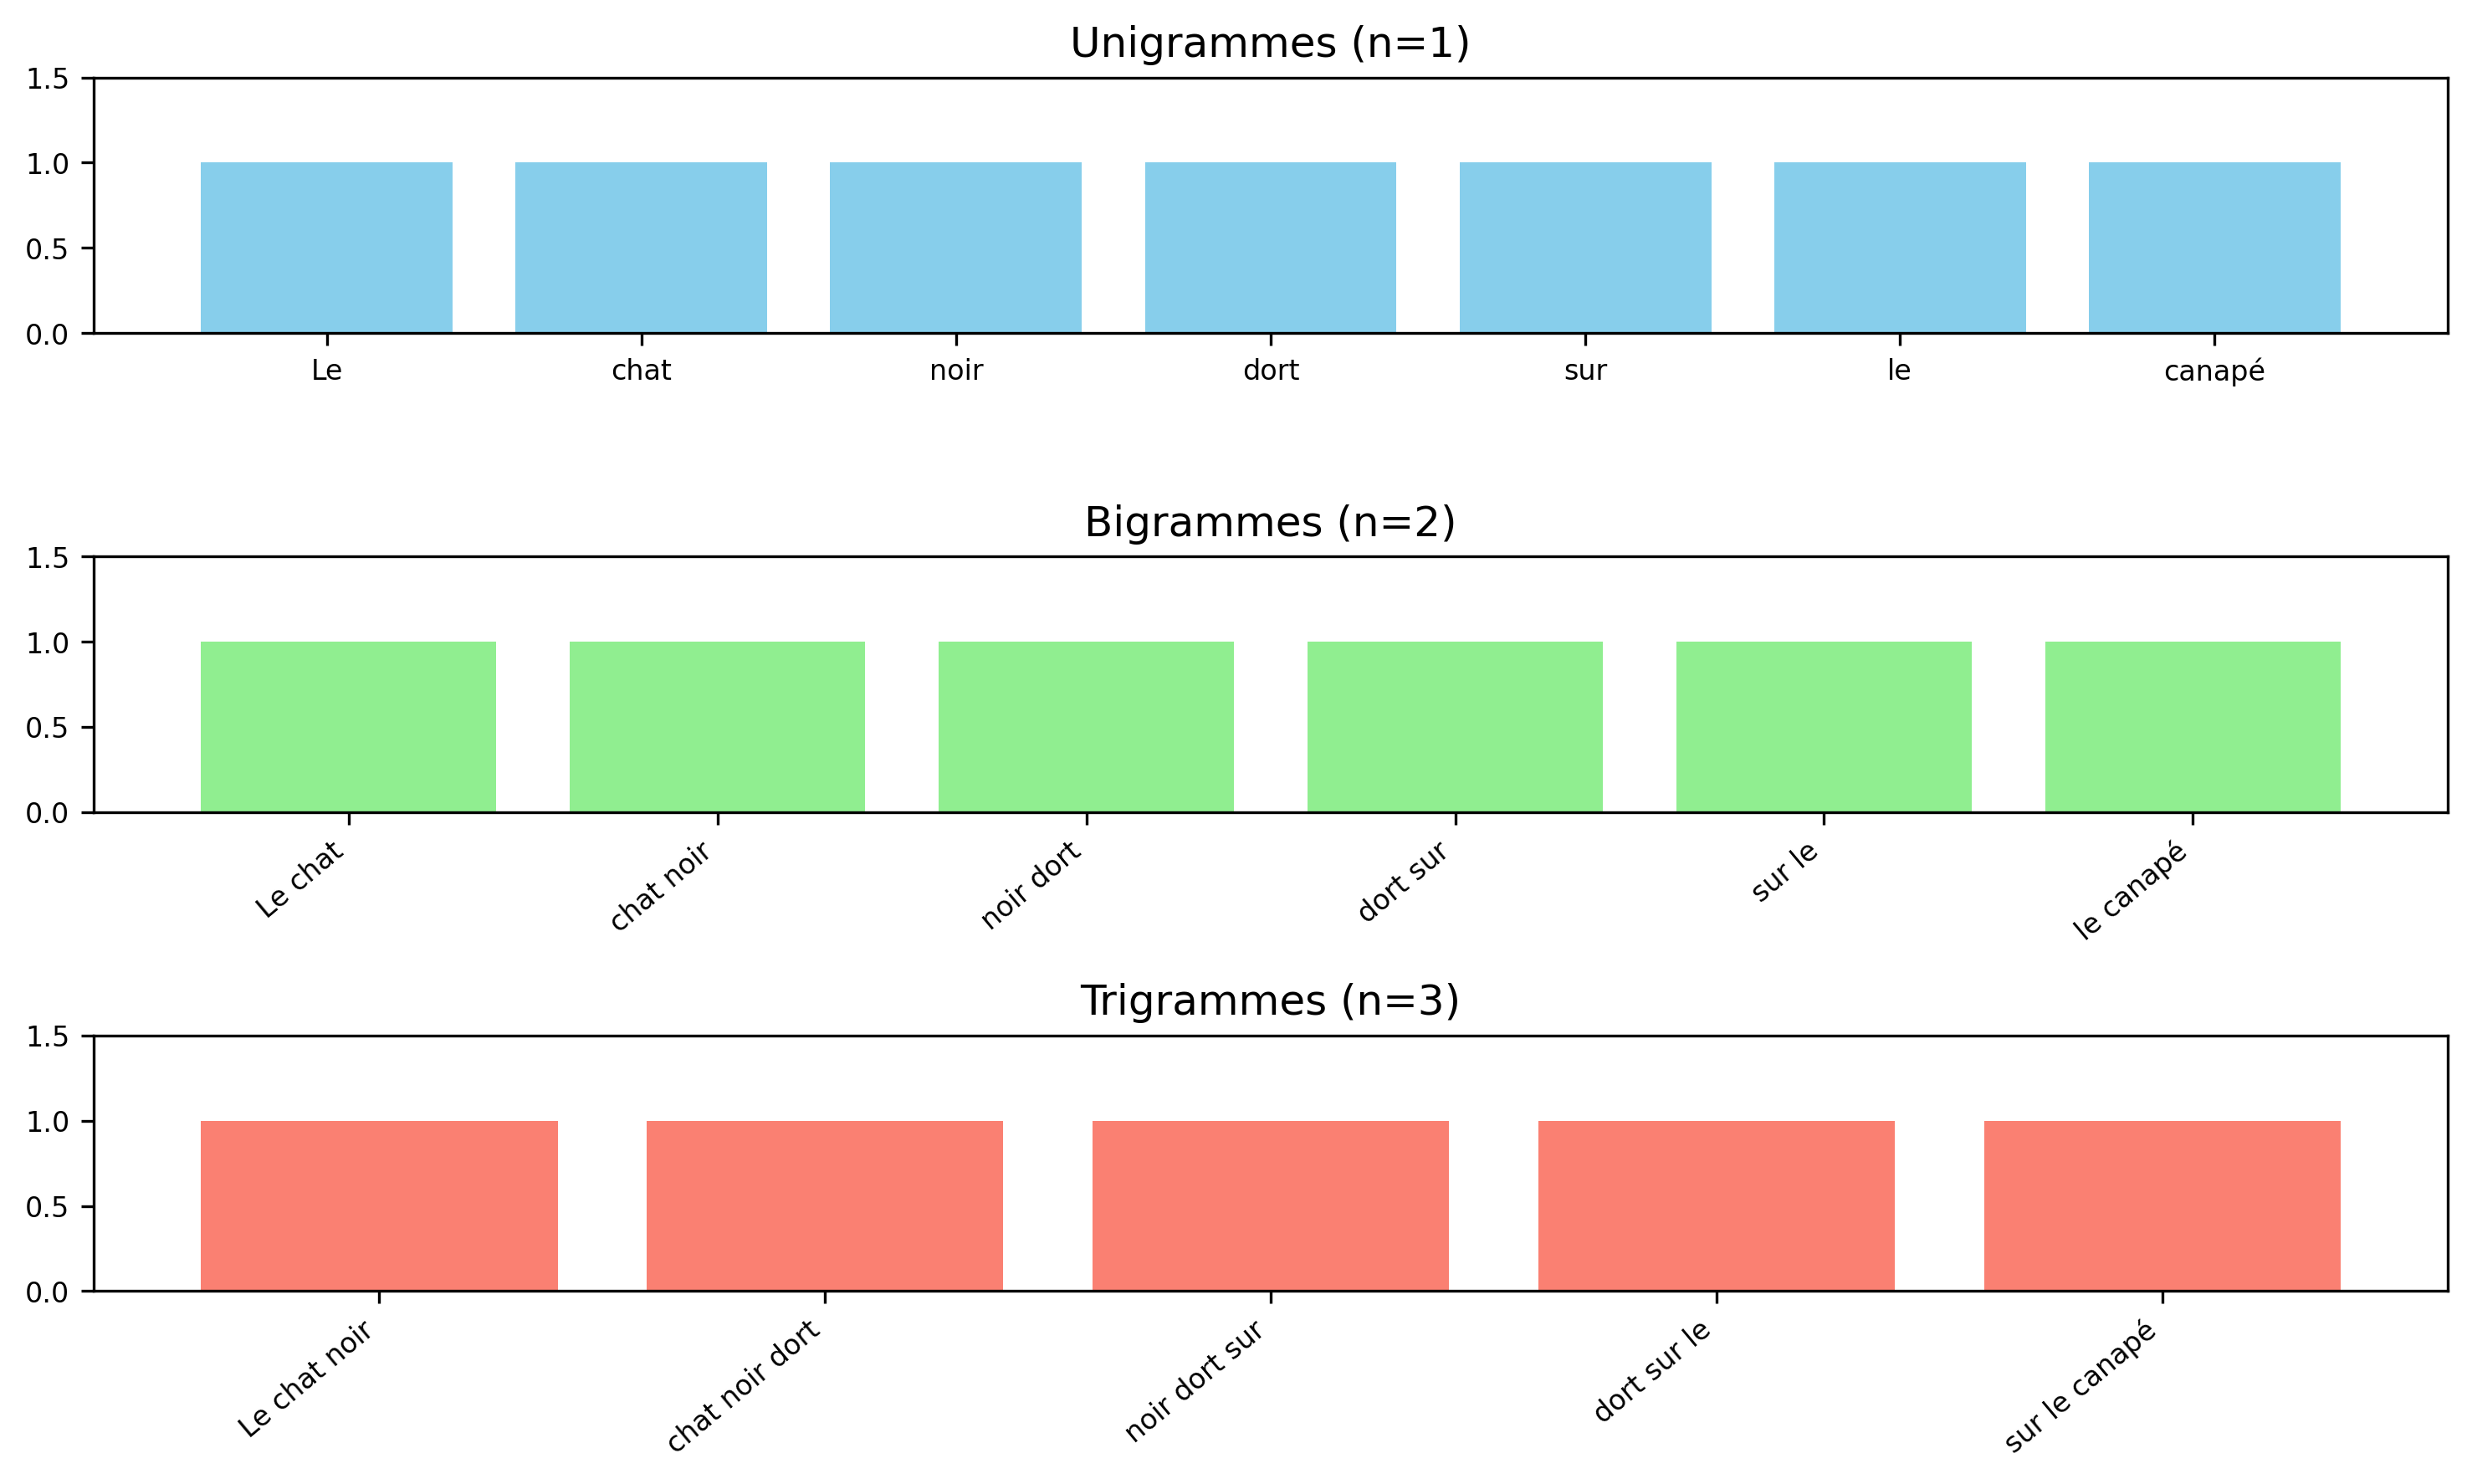
\includegraphics[width=\textwidth]{images/generated/ngram_model.png}
            \vspace{0.1cm}
            \begin{center}
                \small{Exemples d'unigrammes, bigrammes et trigrammes}
            \end{center}
        \end{column}
    \end{columns}
\end{frame}

% Slide: Construction d'un modèle N-gram - Partie 1
\begin{frame}{Construction d'un Modèle N-gram (1/2)}
    \begin{columns}
        \begin{column}{0.5\textwidth}
            \textbf{Étapes de construction}
            \begin{enumerate}
                \item \textbf{Collecte d'un corpus} représentatif
                \item \textbf{Prétraitement} des données textuelles
                \item \textbf{Extraction des n-grams} de taille n
                \item \textbf{Comptage des occurrences} de chaque n-gram
                \item \textbf{Calcul des probabilités conditionnelles}
            \end{enumerate}
            
            \vspace{0.2cm}

        \end{column}
        \begin{column}{0.5\textwidth}
            \textbf{Formule pour bigrammes}:
            \begin{equation}
            P(w_i|w_{i-1}) = \frac{count(w_{i-1}, w_i)}{count(w_{i-1})}
            \end{equation}
            
            \vspace{0.2cm}
            \textbf{Formule générale pour n-grammes}:
            \begin{equation}
            P(w_i|w_{i-n+1}^{i-1}) = \frac{count(w_{i-n+1}^{i})}{count(w_{i-n+1}^{i-1})}
            \end{equation}
        \end{column}
    \end{columns}
\end{frame}

% Slide: Construction d'un modèle N-gram - Partie 2
\begin{frame}{Construction d'un Modèle N-gram (2/2)}
    \begin{columns}
        \begin{column}{0.5\textwidth}
            \textbf{Exemple de construction d'un modèle bigramme}
            
            \textbf{Corpus}: "Le chat noir dort. Le chat blanc joue."
        \end{column}
        \begin{column}{0.5\textwidth}
            \textbf{Bigrammes extraits}:
            \begin{itemize}
                \item (Le, chat): 2 occurrences
                \item (chat, noir): 1 occurrence
                \item (chat, blanc): 1 occurrence
            \end{itemize}
        \end{column}
    \end{columns}
    
    \begin{columns}
        \begin{column}{0.5\textwidth}
            \textbf{Autres bigrammes}:
            \begin{itemize}
                \item (noir, dort): 1 occurrence
                \item (blanc, joue): 1 occurrence
            \end{itemize}
        \end{column}
        \begin{column}{0.5\textwidth}
            \textbf{Probabilités}:
            \begin{itemize}
                \item $P(chat|Le) = \frac{2}{2} = 1.0$
                \item $P(noir|chat) = \frac{1}{2} = 0.5$
                \item $P(blanc|chat) = \frac{1}{2} = 0.5$
            \end{itemize}
        \end{column}
    \end{columns}
\end{frame}

% Slide: Génération de texte avec N-grams
\begin{frame}{Génération de Texte avec N-grams}
    \begin{columns}
        \begin{column}{0.55\textwidth}
            \textbf{Algorithme de génération}
            \begin{enumerate}
                \item \textbf{Choisir un mot/contexte initial}
                \begin{itemize}
                    \item Aléatoirement ou spécifié par l'utilisateur
                \end{itemize}
                \item \textbf{Pour chaque étape de génération}:
                \begin{itemize}
                    \item Identifier les derniers n-1 mots (contexte)
                    \item Consulter la table de probabilités conditionnelles
                    \item Sélectionner le mot suivant selon ces probabilités
                    \item Ajouter ce mot à la séquence générée
                \end{itemize}
                \item \textbf{Répéter} jusqu'à un critère d'arrêt:
                \begin{itemize}
                    \item Longueur maximale atteinte
                    \item Token de fin de phrase/texte généré
                    \item Impossible de continuer (contexte inconnu)
                \end{itemize}
            \end{enumerate}
        \end{column}
        \begin{column}{0.45\textwidth}
            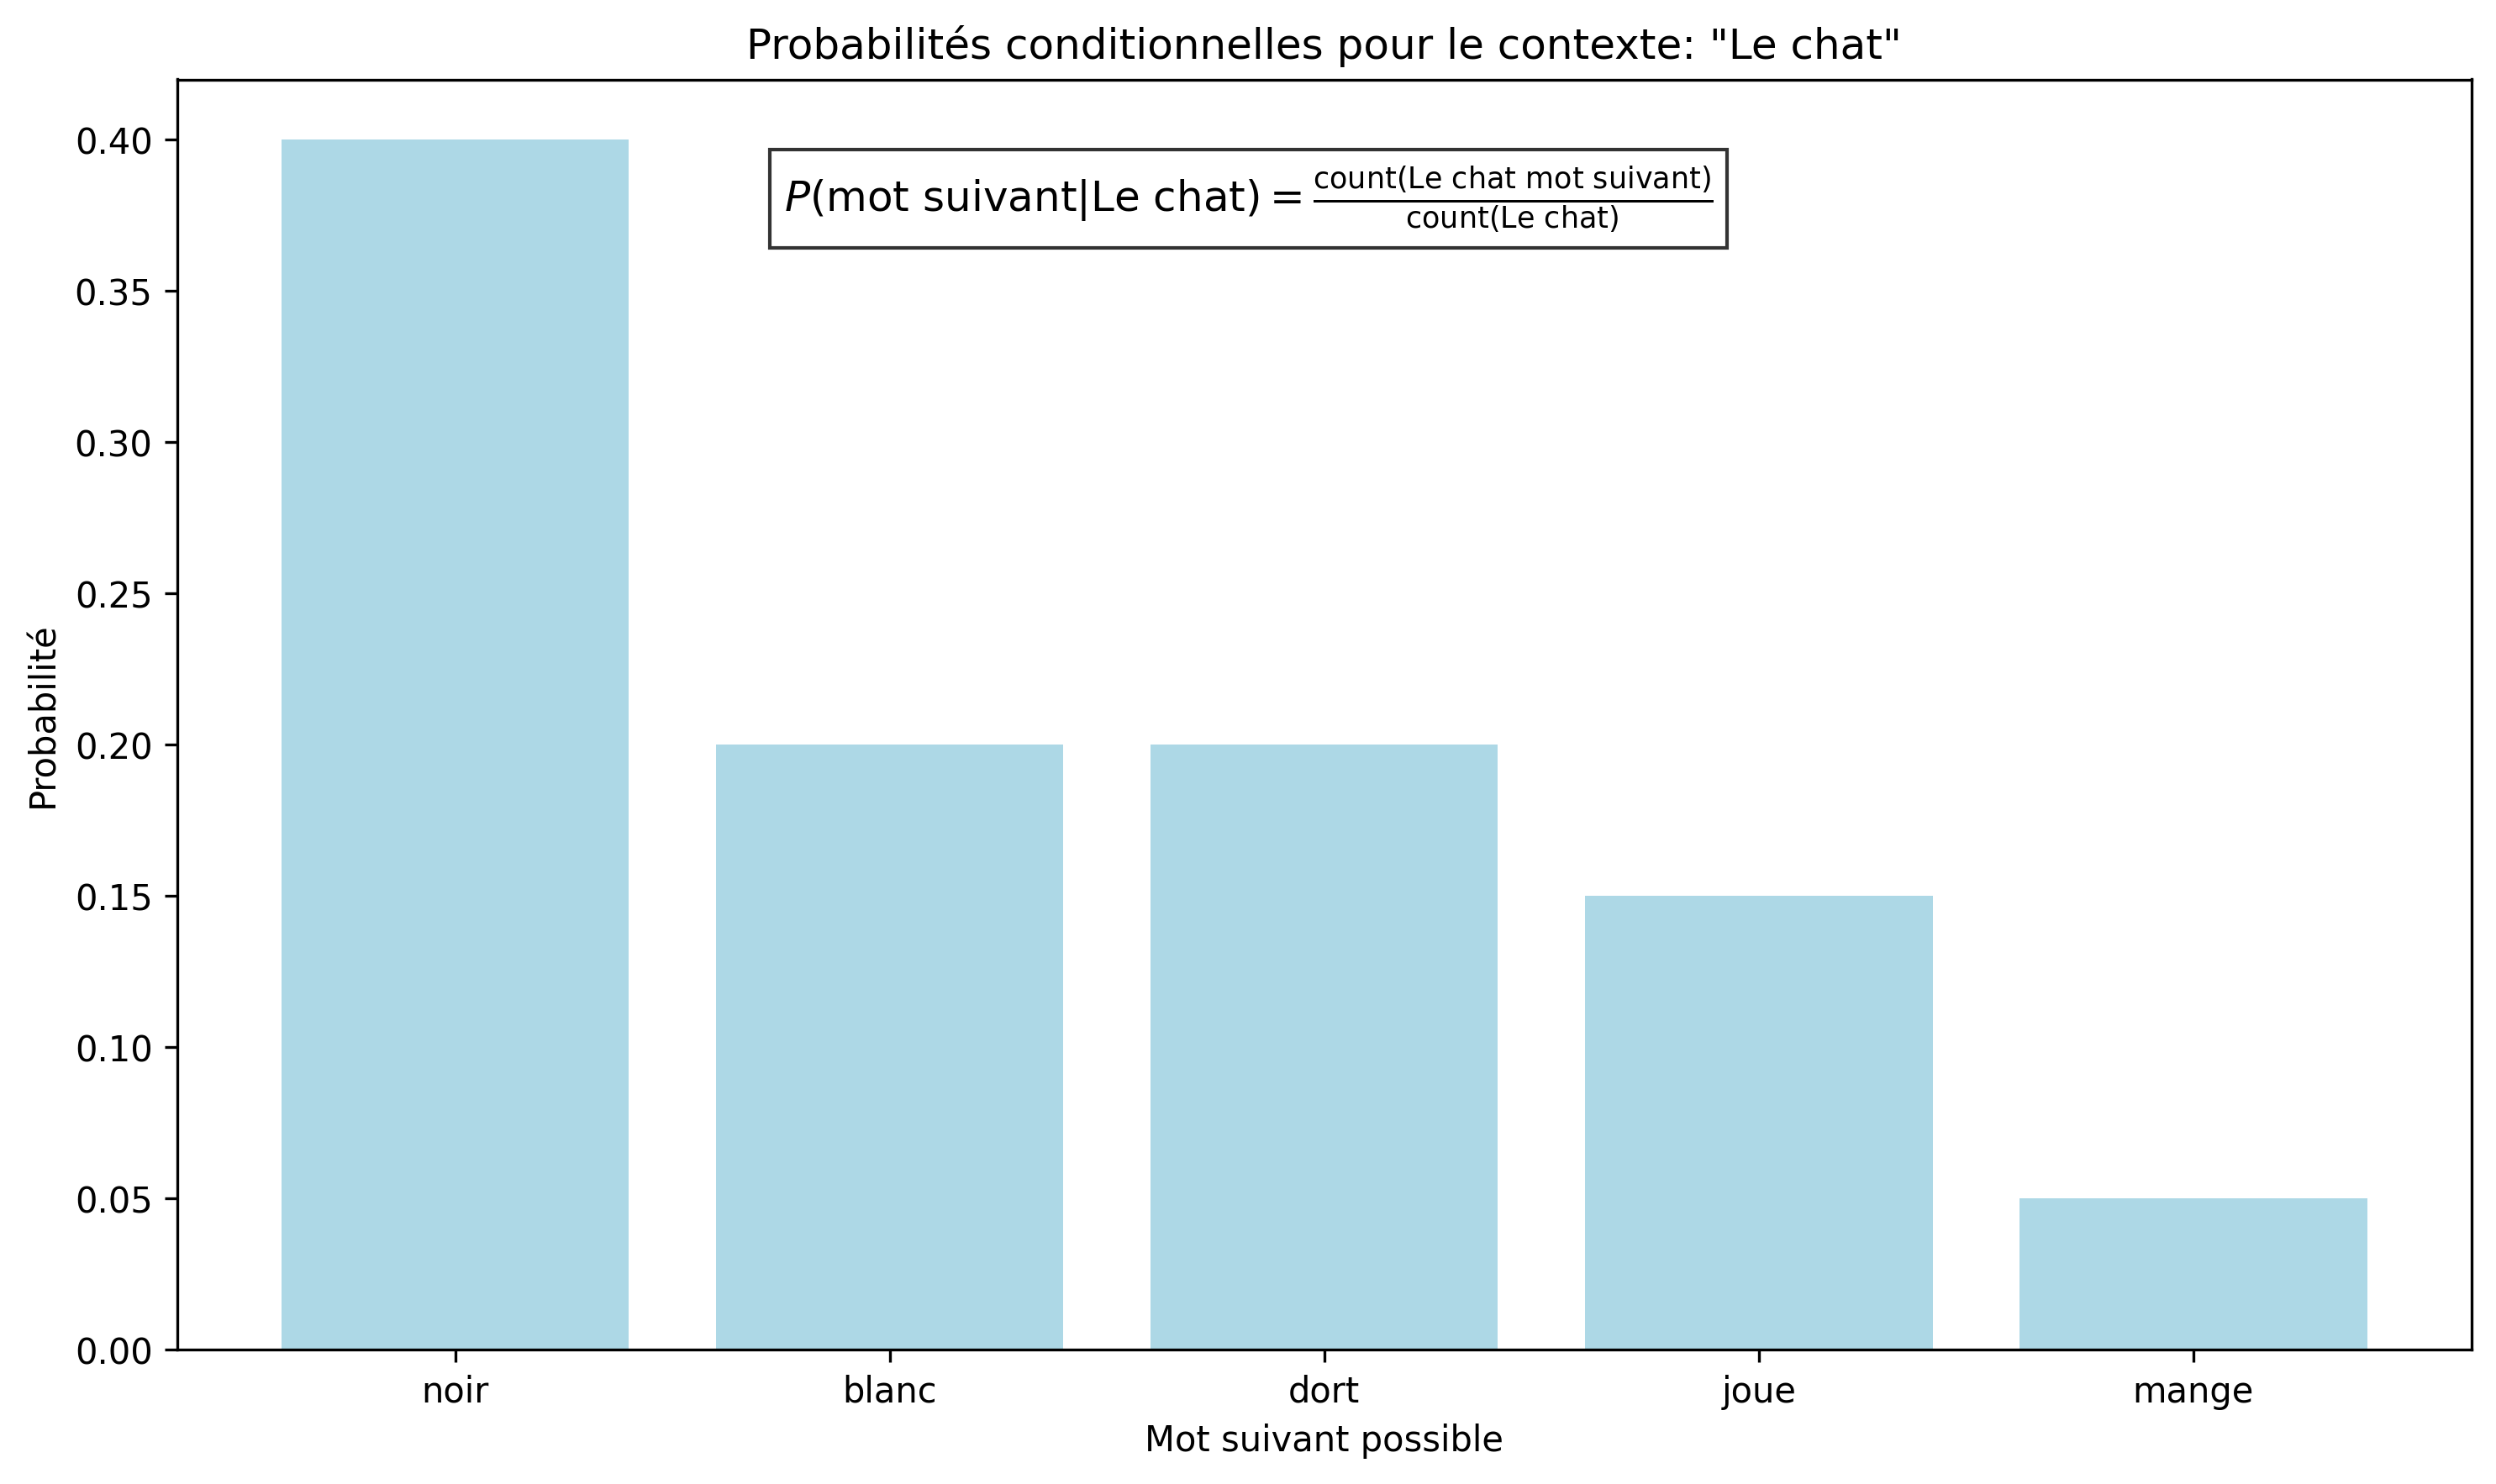
\includegraphics[width=\textwidth]{images/generated/ngram_generation.png}
            \vspace{0.1cm}
            \begin{center}
                \small{Probabilités conditionnelles pour générer le mot suivant}
            \end{center}
        \end{column}
    \end{columns}
\end{frame}

% Slide: Problèmes et améliorations des modèles N-gram
\begin{frame}{Problèmes et Améliorations des Modèles N-gram}
    \begin{columns}
        \begin{column}{0.5\textwidth}
            \textbf{Problèmes fondamentaux}
            \begin{itemize}
                \item \textbf{Données parcimonieuses (sparsity)}
                \begin{itemize}
                    \item De nombreux n-grams valides n'apparaissent jamais dans le corpus
                    \item Probabilité zéro pour les n-grams non observés
                \end{itemize}
                \vspace{0.2cm}
                \item \textbf{Contexte limité}
                \begin{itemize}
                    \item Capture uniquement les dépendances à courte distance
                    \item Perte de cohérence sur de longs textes
                \end{itemize}
                \vspace{0.2cm}
                \item \textbf{Explosion combinatoire}
                \begin{itemize}
                    \item Nombre de n-grams croît exponentiellement avec n
                    \item Stockage et calcul deviennent prohibitifs
                \end{itemize}
            \end{itemize}
        \end{column}
        \begin{column}{0.5\textwidth}
            \textbf{Techniques d'amélioration}
            \begin{itemize}
                \item \textbf{Lissage (smoothing)}
                \begin{itemize}
                    \item Lissage de Laplace (add-one)
                    \item Lissage de Good-Turing
                    \item Lissage de Kneser-Ney
                \end{itemize}
                \vspace{0.2cm}
                \item \textbf{Backoff et interpolation}
                \begin{itemize}
                    \item Utiliser des n-grams plus courts quand les plus longs ne sont pas disponibles
                    \item Combiner les probabilités de différents ordres de n-grams
                \end{itemize}
                \vspace{0.2cm}
                \item \textbf{Modèles de classe}
                \begin{itemize}
                    \item Regrouper les mots en classes sémantiques
                    \item Réduire la parcimonie des données
                \end{itemize}
            \end{itemize}
        \end{column}
    \end{columns}
\end{frame}

% Slide: Exemple concret de génération de texte
\begin{frame}{Exemple Concret de Génération de Texte}
    \begin{exampleblock}{Texte d'entraînement (extrait)}
        \small{Le soleil brille dans le ciel bleu. Les oiseaux chantent dans les arbres. Le vent souffle doucement sur les feuilles. Les enfants jouent dans le parc.}
    \end{exampleblock}
    
    \vspace{0.2cm}
    \begin{columns}
        \begin{column}{0.5\textwidth}
            \textbf{Modèle bigramme (extraits)}
            \begin{itemize}
                \item $P(brille|soleil) = 1.0$
                \item $P(dans|brille) = 1.0$
                \item $P(le|dans) = 1.0$
                \item $P(ciel|le) = 0.25$
                \item $P(parc|le) = 0.25$
                \item $P(vent|le) = 0.25$
                \item $P(souffle|vent) = 1.0$
            \end{itemize}
        \end{column}
        \begin{column}{0.5\textwidth}
            \textbf{Génération à partir du mot "Le"}
            \begin{itemize}
                \item Contexte: "Le"
                \item Choix possibles: "soleil", "vent", "ciel", "parc" (tous avec p=0.25)
                \item Supposons que "soleil" est sélectionné
                \item Nouveau contexte: "soleil"
                \item Mot suivant: "brille" (p=1.0)
                \item Et ainsi de suite...
            \end{itemize}
            
            \textbf{Texte généré possible}:
            \small{"Le soleil brille dans le parc. Les enfants jouent dans les arbres."}
        \end{column}
    \end{columns}
\end{frame}

% Slide: N-grams vs. méthodes modernes
\begin{frame}{N-grams vs. Méthodes Modernes de Génération}
    \begin{columns}
        \begin{column}{0.5\textwidth}
            \textbf{Avantages des N-grams}
            \begin{itemize}
                \item \textbf{Simplicité} conceptuelle et d'implémentation
                \item \textbf{Efficacité} computationnelle (après entraînement)
                \item \textbf{Interprétabilité} des probabilités
                \item \textbf{Peu de données} nécessaires pour des applications simples
                \item \textbf{Domaines spécialisés}: encore utiles pour certaines applications restreintes
            \end{itemize}
        \end{column}
        \begin{column}{0.5\textwidth}
            \textbf{Limites face aux méthodes modernes}
            \begin{itemize}
                \item \textbf{Dépendances à long terme} non capturées
                \item \textbf{Manque de généralisation} sémantique
                \item \textbf{Cohérence} limitée sur de longs textes
                \item \textbf{Compréhension} superficielle du langage
                \item \textbf{Créativité} limitée (reproduit le corpus)
            \end{itemize}
            \vspace{0.3cm}
            \begin{alertblock}{Place des N-grams aujourd'hui}
                Les N-grams restent une \textbf{baseline} importante et sont encore utilisés dans des \textbf{systèmes hybrides}, notamment en combinaison avec des modèles neuronaux plus avancés.
            \end{alertblock}
        \end{column}
    \end{columns}
\end{frame}
% Slide: Implémentation pratique des N-grams
\begin{frame}{Implémentation Pratique des Modèles N-gram}
    \begin{center}
        \textbf{Implémentation d'un modèle N-gram en Python}
    \end{center}
\end{frame}


% Slide: Limites et transition vers les techniques modernes
\begin{frame}{Au-delà des Approches Traditionnelles}
    \begin{columns}
        \begin{column}{0.45\textwidth}
            \textbf{Limites des méthodes bag-of-words}
            \begin{itemize}
                \item Ne capturent pas la \textbf{sémantique} du langage
                \item Difficultés avec la \textbf{négation}: "pas bon" vs "bon"
                \item Ne gèrent pas bien le langage \textbf{figuratif} (sarcasme, ironie)
                \item Sensibles au \textbf{domaine}: modèle entraîné sur des critiques de films peut mal fonctionner sur des critiques de restaurants
                \item \textbf{Dimensionnalité} élevée avec de grands vocabulaires
            \end{itemize}
        \end{column}
        
        \begin{column}{0.55\textwidth}
            \textbf{Évolutions vers les méthodes modernes}
            \begin{itemize}
                \item \textbf{Word Embeddings} (Word2Vec, GloVe)
                \begin{itemize}
                    \item Représentations denses et continues des mots
                    \item Capture des relations sémantiques
                \end{itemize}
                \item \textbf{Réseaux de neurones récurrents}
                \begin{itemize}
                    \item LSTM et GRU pour capturer les séquences
                \end{itemize}
                \item \textbf{Architectures Transformer}
                \begin{itemize}
                    \item BERT, RoBERTa pour l'analyse contextuelle
                    \item GPT pour la génération et classification
                \end{itemize}
                \item \textbf{Méthodes multimodales}
                \begin{itemize}
                    \item Analyse conjointe du texte et d'autres signaux
                \end{itemize}
            \end{itemize}
        \end{column}
    \end{columns}
\end{frame}

% New section on the future of LLMs
\section{Le Futur des Modèles de Langage (LLMs)}

% Slide: Introduction to LLMs and their evolution
\begin{frame}{Évolution des Modèles de Langage à Grande Échelle}
    \begin{itemize}
        \item Les \textbf{Large Language Models (LLMs)} représentent une avancée majeure en NLP
        \item \textbf{Évolution rapide} depuis 2018:
        \begin{itemize}
            \item GPT-1 (0.1B paramètres) $\rightarrow$ GPT-4 ($>$1T paramètres estimés)
            \item Augmentation de la taille des modèles = capacités émergentes
        \end{itemize}
        \item \textbf{Capacités actuelles}:
        \begin{itemize}
            \item Génération de texte cohérent et contextuel
            \item Adaptation à différentes tâches sans fine-tuning spécifique
            \item Compréhension complexe et résolution de problèmes
            \item Génération de code, traduction avancée, créativité
        \end{itemize}
        \item Ces modèles transforment comment nous \textbf{interagissons avec l'information} et \textbf{automatisons les tâches cognitives}
    \end{itemize}
\end{frame}

% Slide: Advanced reasoning capabilities of LLMs
\begin{frame}{Capacités de Raisonnement Avancées}
    \begin{columns}
        \begin{column}{0.55\textwidth}
            \textbf{Émergence du raisonnement complexe}
            \begin{itemize}
                \item \textbf{Test-Time Scaling}: Amélioration des performances avec plus de temps d'inférence
                \begin{itemize}
                    \item Chain-of-Thought (CoT): raisonnement étape par étape
                    \item Tree-of-Thoughts (ToT): exploration de multiples voies de raisonnement
                    \item Self-consistency: génération de plusieurs solutions et vote majoritaire
                \end{itemize}
                \vspace{0.3cm}
                \item \textbf{Émergence avec l'échelle}
                \begin{itemize}
                    \item Les capacités émergent non-linéairement avec la taille du modèle
                    \item Point critique où le raisonnement "apparaît"
                \end{itemize}
            \end{itemize}
        \end{column}
        \begin{column}{0.45\textwidth}
            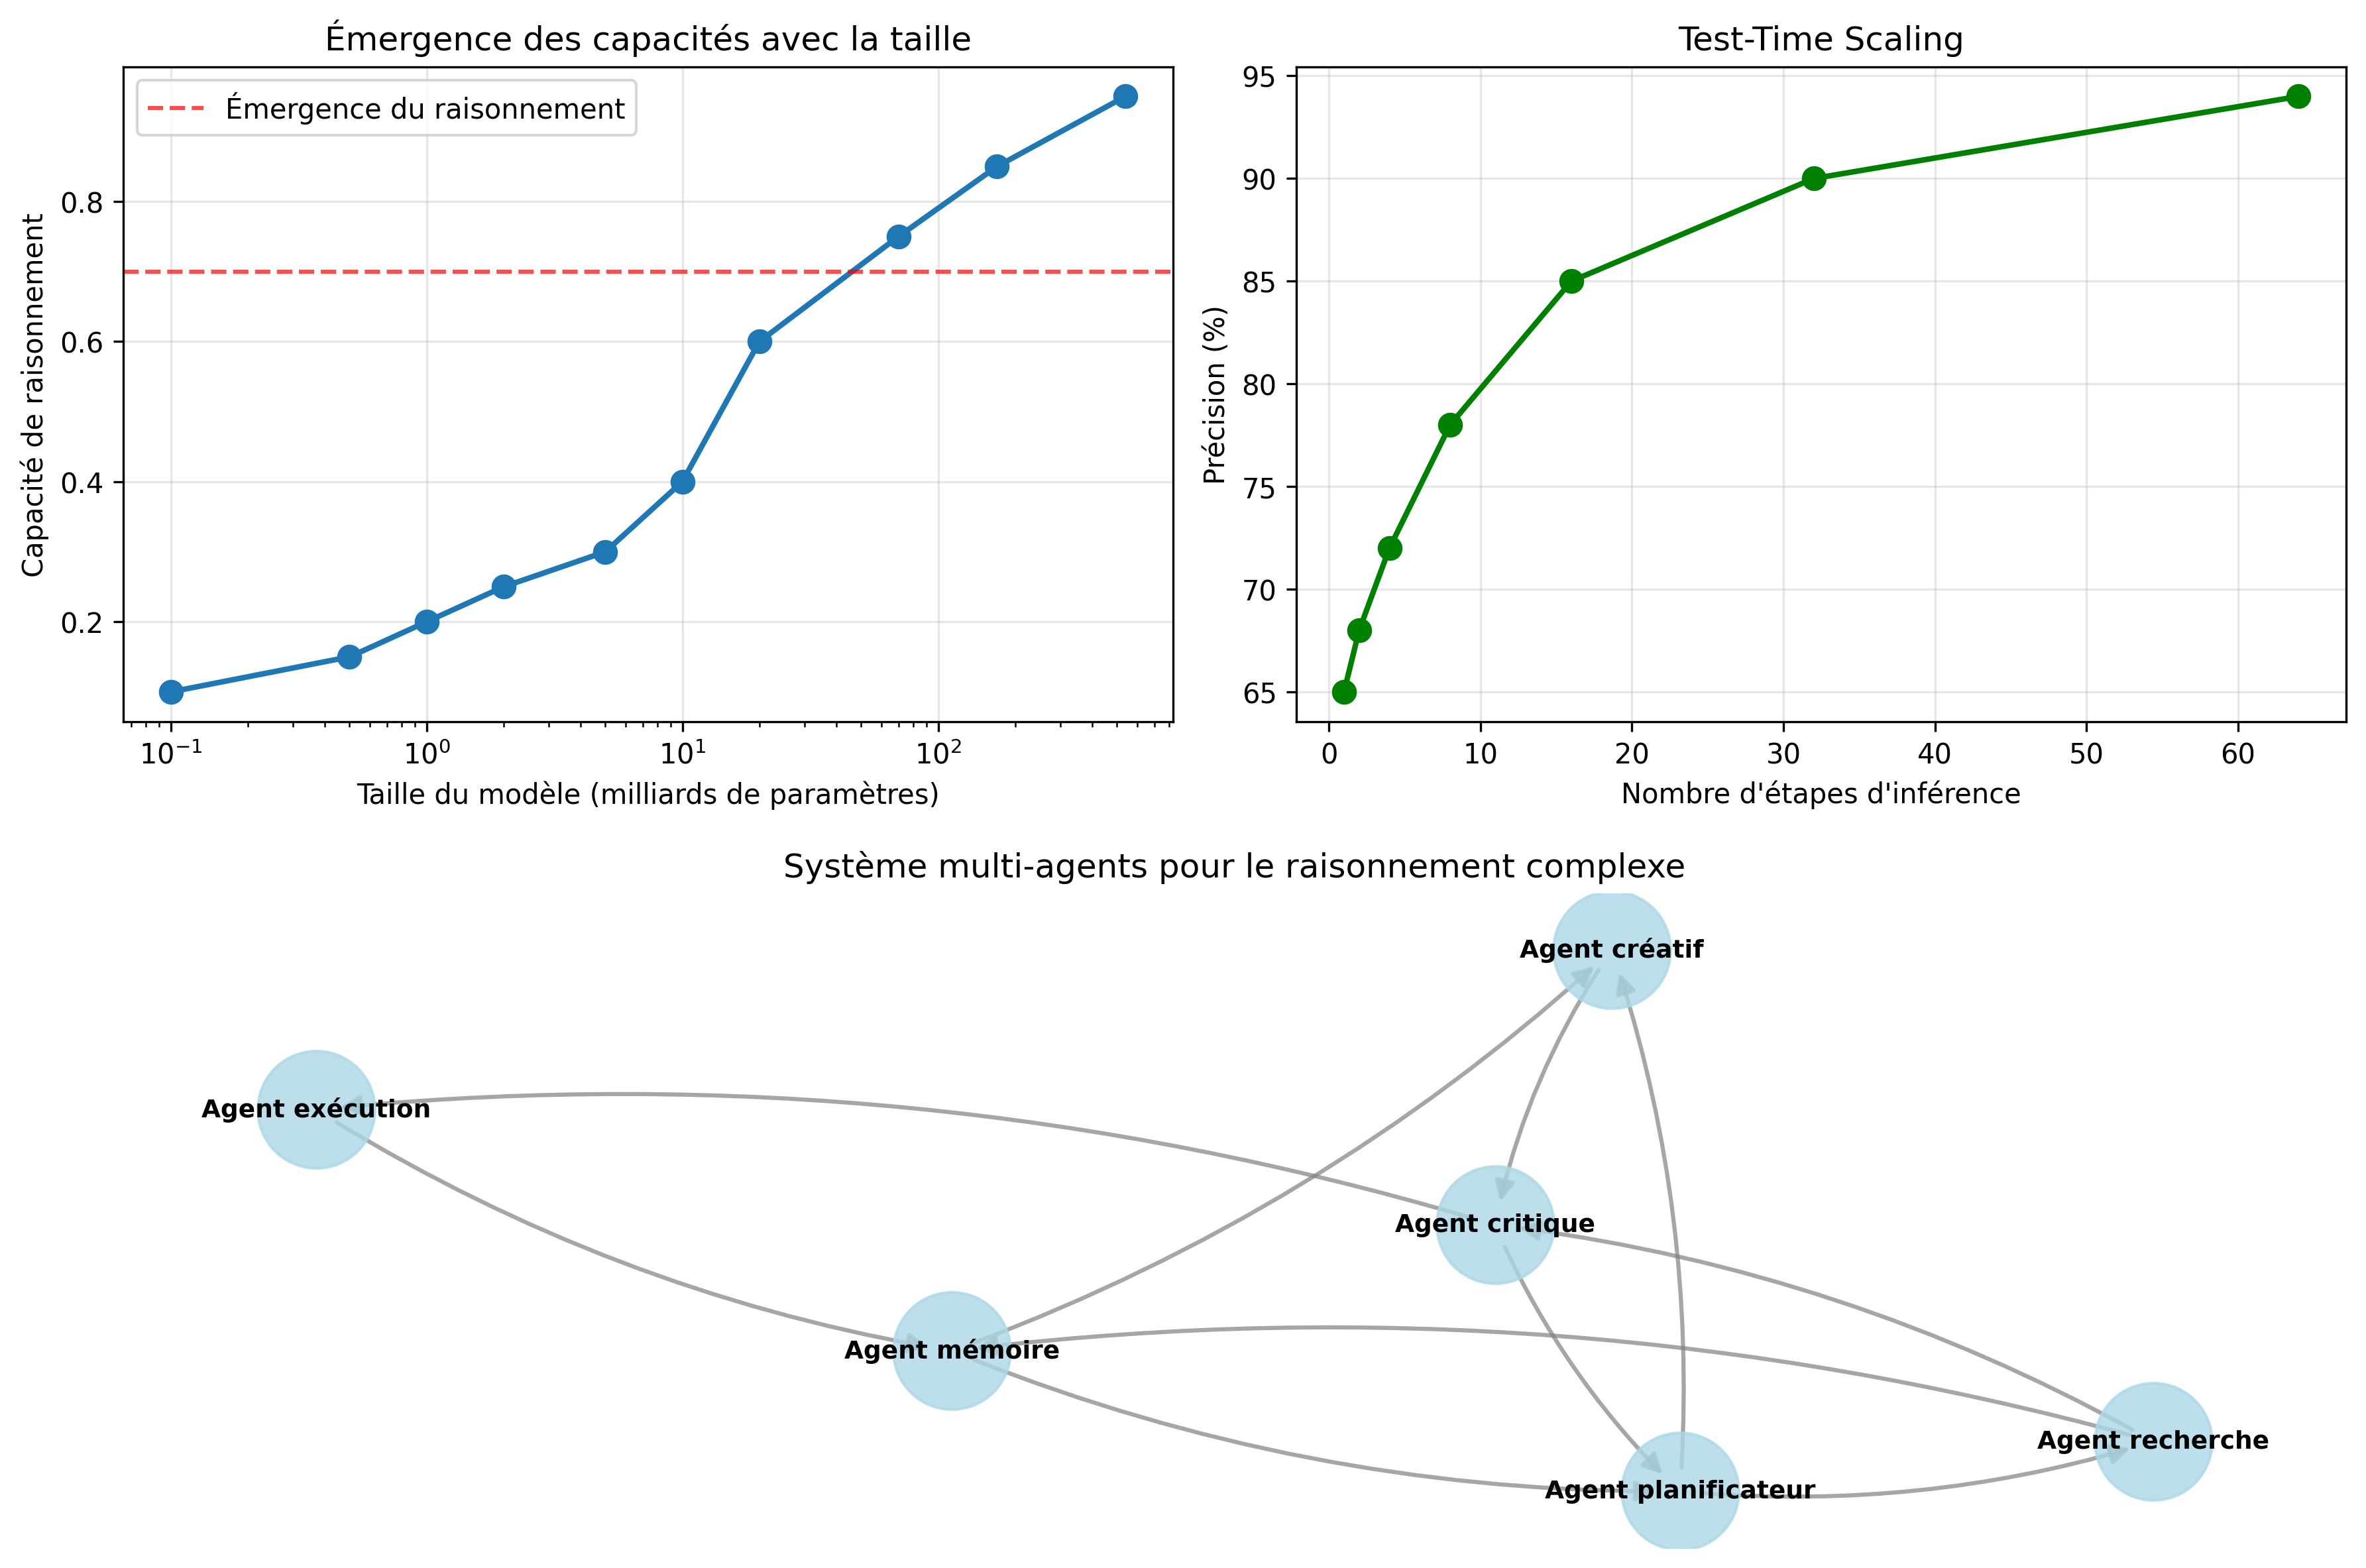
\includegraphics[width=\textwidth]{images/generated/llm_future.png}
            \vspace{0.2cm}
            \begin{center}
                \small{Émergence des capacités et test-time scaling}
            \end{center}
        \end{column}
    \end{columns}
\end{frame}

% Slide: Agent systems and complex interactions
\begin{frame}{Systèmes d'Agents: Intelligence Collective}
    \begin{itemize}
        \item \textbf{Systèmes multi-agents}:
        \begin{itemize}
            \item Plusieurs LLMs spécialisés collaborant sur des tâches complexes
            \item Chaque agent possède un rôle spécifique: planification, critique, recherche, etc.
            \item Communication inter-agents pour résoudre des problèmes multi-étapes
        \end{itemize}
        \vspace{0.3cm}
        \item \textbf{Avantages}:
        \begin{itemize}
            \item \textbf{Auto-correction}: les agents peuvent se critiquer mutuellement 
            \item \textbf{Diversité de perspectives}: différentes approches pour un même problème
            \item \textbf{Spécialisation}: agents optimisés pour certaines tâches spécifiques
            \item \textbf{Réduction des hallucinations}: vérification croisée des informations
        \end{itemize}
        \vspace{0.3cm}
        \item Applications: recherche scientifique, résolution de problèmes complexes, diagnostic médical, création de contenu
    \end{itemize}
\end{frame}

% Slide: Current challenges and future directions
\begin{frame}{Défis Actuels et Directions Futures}
    \begin{columns}
        \begin{column}{0.48\textwidth}
            \textbf{Défis}
            \begin{itemize}
                \item \textbf{Hallucinations}: génération d'informations incorrectes
                \item \textbf{Biais et équité}: reproduction de biais présents dans les données
                \item \textbf{Alignement}: garantir que les modèles agissent selon les valeurs humaines
                \item \textbf{Efficacité énergétique}: réduire l'empreinte environnementale
                \item \textbf{Sécurité}: prévenir les usages malveillants
            \end{itemize}
        \end{column}
        \begin{column}{0.52\textwidth}
            \textbf{Directions de recherche}
            \begin{itemize}
                \item \textbf{Modèles plus petits mais spécialisés}
                \item \textbf{Apprentissage continu} à partir de l'interaction humaine
                \item \textbf{Intégration de connaissances externes} (outils, bases de données)
                \item \textbf{Amélioration de l'interprétabilité} des modèles
                \item \textbf{Multilinguisme} et accessibilité mondiale
                \item \textbf{Multimodalité}: vision, audio, texte combinés
            \end{itemize}
        \end{column}
    \end{columns}
    \vspace{0.3cm}
    \begin{center}
        \textbf{Le futur du NLP se dirige vers des systèmes hybrides intégrant LLMs, bases de connaissances, et outils spécialisés}
    \end{center}
\end{frame}

\end{document} 